\chapter{动力问题的完全弱形式时空混合有限元法}\label{ch:1dimension}

本章基于弹性波动力问题在复杂求解域难以进行解析求解，
通常需要采用有限元等数值近似方法模拟波在介质中的传播过程，
分析了时间域和空间域分开进行近似离散的两种常用方法以及弊端。
时间域属于初值问题，基于强形式采用迭代方法对时域进行积分；
空间域属于边值问题，基于哈密顿原理的完全弱形式伽辽金法进行求解。
在此基础上，结合两种方法通过哈密顿原理将时间域和空间域同时采用有限元形函数进行离散，
并详细阐述了基于哈密顿原理的时空混合离散法在时间末端边界条件问题的解决方法，
建立一个在有限元伽辽金数值计算中能自适应时空混合离散的方案。

\section{动力问题及基于强形式的迭代求解}

在拉格朗日力学当中，动力问题可通过变分原理或称哈密顿原理(Hamilton’s Principle)进行描述。
哈密顿原理指出，系统的真实运动轨迹会使能量泛函取极值，能量泛函的表达式为：
\begin{equation}\label{eq:functional}
    \Phi(q) = \int_{t_0}^{t_1} L(q, \dot{q}, t) dt
\end{equation}
其中，$q$和$\dot q$为广义自由度和其对时间$t$的一阶导数。
$L$为拉格朗日量，其表达式为：
\begin{equation}\label{eq:lagrangian}
    L = T - U
\end{equation}
式中，$T$为动能，$U$为势能。
根据哈密顿原理\cite{arnold1978}，该问题的精确解$q$使得式\eqref{eq:functional}的变分等于$0$，即：找到一个$q\in \mathcal{Q}$，使得
\begin{equation}\label{eq:variation}
    \begin{aligned}
        \delta \Phi(q) &= \int_{t_0}^{t_1} \left( \frac{\partial L}{\partial q} \delta q + \frac{\partial L}{\partial \dot{q}} \delta \dot{q} \right) dt \\
        &= \int_{t_0}^{t_1} \left( \frac{\partial L}{\partial q} - \frac{d}{dt} \frac{\partial L}{\partial \dot{q}} \right) \delta q \, dt + \left. \frac{\partial L}{\partial \dot{q}} \delta q \right|_{t_0}^{t_1} \\ &= 0
    \end{aligned}
    \quad \forall \delta q \in \mathcal{Q}'
\end{equation}
其中，$\mathcal{Q}$为试函数空间满足$q\in \mathcal{Q}$，$q_0$和$\dot q_0$为$q$在$t_0$时刻的初始位移和速度。
而$\mathcal{Q}'$为权函数空间$\mathcal{P}$，满足$\delta q\in \mathcal{Q}'$。
根据$\mathcal{P}$的定义，可得到如下所示欧拉-拉格朗日方程：
\begin{equation}\label{eq:euler-lagrange}
    \frac{\partial L}{\partial q} - \frac{d}{dt} \frac{\partial L}{\partial \dot{q}} = 0
\end{equation}

通常情况下，此类动力问题已知初始条件$q(t_0)=q_0$和$\dot{q}(t_0)=\dot{q}_0$，所以也称为初值问题。
欧拉-拉格朗日相较于哈密顿原理中的式\eqref{eq:variation}对解的要求更高，式\eqref{eq:euler-lagrange}要求在时间域$(t_0,t_1)$内处处成立，而式\eqref{eq:variation}只要求对全域积分后下成立。
所以可以称式\eqref{eq:euler-lagrange}为强形式方程(\textbf{Strong Form})，
而式\eqref{eq:variation}为弱形式方程(\textbf{Weak Form})。

\begin{figure}[!h]
    \centering
    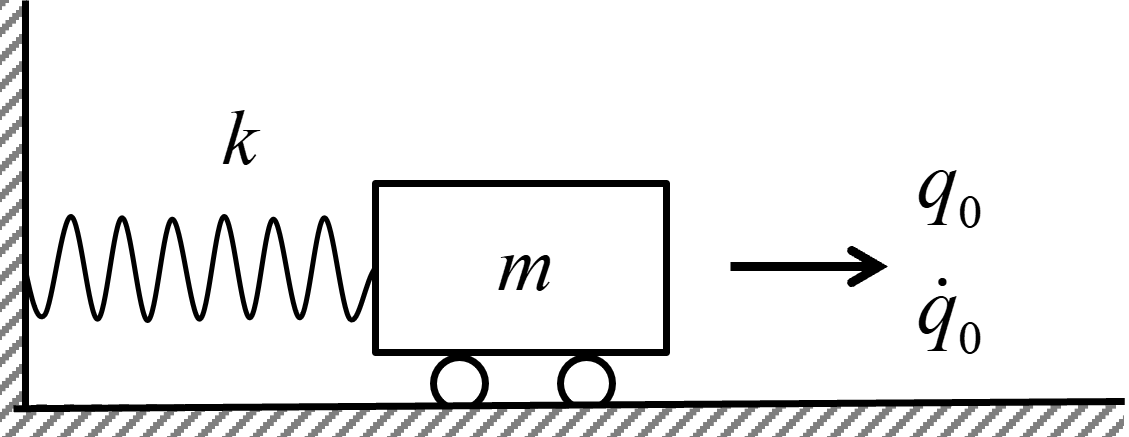
\includegraphics[scale=1.0]{fig/math/弹簧小车模型.png}
\caption{\centering{一维弹簧小车算例模型}}
\label{fg:2.3}
\end{figure}

不失一般性，我们考虑如图\ref{fg:2.3}所示的一维弹簧小车问题，展示如何求解动力问题。
在弹簧小车问题中式\eqref{eq:lagrangian}中的动能$T$和势能$U$具有如下表达式：
\begin{equation}\label{eq:kinetic-potential}
    T = \frac{1}{2} m \dot{q}^2, \quad U = \frac{1}{2} k q^2
\end{equation}
其中，$m$表示小车质量，$k$表示刚度系数，$\ddot q$为广义自由度对时间$t$的二阶导数。

对此类问题的时间域分析，常采用基于欧拉-拉格朗日方程强形式的离散方法(如有限差分法)，
将式\eqref{eq:kinetic-potential}代入式\eqref{eq:euler-lagrange}可得该问题的平衡微分方程为：
\begin{equation}\label{2.1}
m \ddot q + k q =0
\end{equation}

Newmark-$\beta$法是基于时间导数的有限差分近似构建的线性动力系统数值积分算法,
通过当前时刻(第$n$步)的状态(位移$q_n$、速度$\dot q_n$​、加速度$\ddot q_n$)，
计算下一时刻(第$n+1$步)的状态，迭代公式中$\Delta t$为时间步长，
$m$为质量，$c$为阻尼系数，$k$为刚度，$f_{n+1}$为第$n+1$步外力。
当取$\gamma=0$、$\beta=0$时，Newmark-$\beta$法为显式格式，
采用向前差分近似时间导数，仅利用当前时刻(第$n$步)的状态计算下一时刻(第$n+1$步)状态，
无需求解方程组，迭代公式为：
\begin{equation}\label{newmark-explicit}
    \left \{
        \begin{split}
            \ddot q_n &= \frac{1}{m}(f_n - c \dot q_n - k q_n) \\
            \dot q_{n+1} &= \dot q_n + \Delta t \ddot q_n \\
            q_{n+1} &= q_n + \Delta t \dot q_n
        \end{split}
    \right .
\end{equation}

当取$\gamma=1$、$\beta=\frac{1}{2}$时，Newmark-$\beta$法为隐式格式，
采用向后差分近似时间导数，利用下一时刻(第$n+1$步)的状态反推更新，
需通过求解线性方程组获取未知状态，迭代公式为：
\begin{equation}\label{newmark-implicit}
    \left \{
        \begin{split}
            \ddot q_{n+1} &= \frac{1}{m}(f_{n+1} - c \dot q_{n+1} - k q_{n+1}) \\
            \dot q_{n+1} &= \dot q_n + \Delta t \ddot q_{n+1} \\
            q_{n+1} &= q_n + \Delta t \dot q_{n+1}
        \end{split}
    \right .
\end{equation}

当取$\gamma=1$、$\beta=0$时，Newmark-$\beta$法为半隐式格式，
结合向前差分与向后差分特点：加速度依赖当前时刻位移简化计算，
速度和位移采用下一时刻加速度更新以提升稳定性，迭代公式为：
\begin{equation}\label{newmark-semi-implicit}
    \left \{
        \begin{split}
            \ddot q_{n+1} &= \frac{1}{m}(f_{n+1} - c \dot q_{n+1} - k q_n) \\
            \dot q_{n+1} &= \dot q_n + \Delta t \ddot q_{n+1} \\
            q_{n+1} &= q_n + \Delta t \dot q_{n+1}
        \end{split}
    \right .
\end{equation}

综上所述，Newmark-$\beta$迭代法的三种形式，都是对时间域采用基于微分方程的强形式进行离散分析，
差别在于对时间导数的差分近似方式。同时三种形式有各自的优缺点，就如章节\ref{ch:wznthxc}所示的无阻尼弹簧小车算例。
显式算法依赖当前时刻信息，计算无需求解方程组，计算效率高，但计算结果存在数值色散现象，计算结果也不稳定；
隐式算法依赖未来时刻信息，属于无条件稳定范畴，但计算结果存在严重的数值耗散现象(Numerical dissipation)；
半隐式算法则混合使用两类信息，在计算效率与稳定性之间取得平衡，可以做到条件稳定，得到较好的计算结果。










\section{基于哈密顿原理的完全弱形式求解}

基于哈密顿原理的完全弱形式\eqref{eq:variation}进行求解，
% 将时间域作为第四维空间，
% 并采用基于哈密顿原理的伽辽金弱形式协同空间区域进行混合离散，
% 称为时空混合离散伽辽金法。
该方法是一种从系统能量变分本质出发，
对动力问题(包括弹性波传播等)进行全域时空离散的数值方法。
其核心思想是通过构建包含空间变量与时间变量的作用量泛函，
利用变分原理将动力系统的控制方程，如欧拉-拉格朗日方程或哈密顿正则方程，
转化为全域范围内的弱形式，从而实现空间域与时间域的统一求解，
避免了传统迭代方法中时间域与空间域分别离散的局限性。
这种方法的显著特点是时空全域离散，即同时对空间域和时间域进行离散化处理，
无需像传统迭代方法那样在时间步内逐次递推，
理论上可一次性求解所有时空节点的状态变量，
因此具备高度并行计算的能力，能够大幅提升计算效率。
同时，时空混合离散网格局部细化过程易于实现，
空间区域的局部细化将不会对后续时间区域构成影响。

在拉格朗日力学中，动力问题需满足变分原理或称哈密顿原理(Hamilton's Principle)。
哈密顿原理指出，系统的真实运动轨迹会使能量泛函取极值，
即动能与势能之差在时间区间上的积分取极值。也就是说能量泛函的变分等于零。
然而，直接采用式\eqref{eq:variation}通常遇到以下问题:
试函数空间$\mathcal{Q}$和权函数空间$\mathcal{P}$并不相同，尤其是在时间末端$t_1$处，$q(t_1)$通常是未知的，而$\delta q(t_1)=0$，这导致在数值实现时难以处理时间末端的边界条件。
并且，初始时刻$t_0$的边界条件同时具有$q(t_0)=q_0$和$\dot q(t_0)=\dot q_0$两个边界条件，如何在弱形式\eqref{eq:variation}的同一时刻施加两个边界条件也是一个难题。

采用传统有限元法进行分析时，对广义变量$q$进行有限元近似，其近似值$q^h$具有如下表达式：
\begin{equation}\label{q_h}
q^h = \sum_{I=1}^{n_p} N_I d_I
\end{equation}
其中，$N_I$为时间域的形函数，$d_I$为对应的节点系数，$n_p$为时间域节点总数。
广义坐标对时间的一阶导数的近似值$\dot q_h$为：
\begin{equation}\label{dotq_h}
    \dot q^h = \sum_{I=1}^{n_p} N_{I,t} d_I
\end{equation}
式中，$N_{I,t}$为形函数对时间的导数。
将动能和势能表达式\eqref{eq:kinetic-potential}代入到弱形式\eqref{eq:variation}，可得如下问题：找到一个$q^h\in \mathcal{Q}^h$，使得
\begin{equation}\label{eq:discrete-variation}
    \int_{t_0}^{t_1} \left( \delta \dot q^h m \dot q^h - \delta q^h k q^h \right) dt = \left. \delta q^h m \dot q^h \right|_{t=t_0} \quad \forall \delta q^h \in \mathcal{P}^h
\end{equation}
其中，$\mathcal Q^h$为有限元近似空间：
\begin{equation}
    \mathcal Q^h = \textrm{span} \{N_I\}_{I=1}^{n_p}
\end{equation}

值得注意的是，为了施加初始时刻动量边界条件，此时的近似权函数空间$\mathcal{P}^h$需要满足$\delta q^h(t_1)=0$，但不再要求$\delta q^h(t_0)=0$，即：
\begin{equation}
    \mathcal P^h = \{q^h \in \mathcal Q^h \vert \delta q^h(t_1) = 0\}
\end{equation}
将有限元近似表达式\eqref{q_h}和式\eqref{dotq_h}代入弱形式\eqref{eq:variation}，
可得到离散控制方程为：
\begin{equation}\label{2.15}
\boldsymbol K \boldsymbol d = \boldsymbol f
\end{equation}
其中，$\boldsymbol K$为刚度矩阵，其分量$K_{IJ}$的表达式为：
\begin{equation}\label{K_IJ}
K_{IJ} = \int_{t_0}^{t_1} N_{I,t} m N_{J,t} - N_I k N_J dt
\end{equation}
而外力向量$\boldsymbol f$施加初始时刻动量边界条件，其分量$f_I$的表达式为：
\begin{equation}\label{f_I}
    f_I = N_I m \dot q_0 |_{t=t_0}
\end{equation}

在使用伽辽金法进行求解的过程中，试函数空间$\mathcal{Q}^h$和权函数空间$\mathcal{P}^h$采用相同的节点数进行离散，即$\dim \mathcal{Q}^h = \dim \mathcal{P}^h$。
然而，如图\ref{fg:δq=0}所示，直接令$q(t_1)=0$，将导致刚度矩阵$\boldsymbol K$不为方阵。
同时，初始时刻已施加边界条件$\dot q(t_0)=\dot q_0$，此时再通过强制方法，如罚函数法，施加$q(t_0)=q_0$边界条件，将导致自然边界条件$\dot q(t_0)=\dot q_0$不起作用。

\begin{figure}[!h]
    \centering
    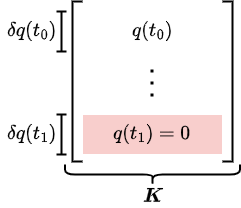
\includegraphics[scale=0.6]{fig/math/末端边界条件等于0图.png}
\caption{\centering{直接施加时域末端虚位移等于零边界条件}}
\label{fg:δq=0}
\end{figure}

为解决上述问题，Peters\cite{peters1988}提出，将初始时刻的本质边界条件$q(t_0)=q_0$直接施加到时间末端$t_1$位置。
这样既能施加初始时刻的本质边界条件，又能保证刚度矩阵为方阵，从而实现数值求解。
然而，该方法存在明显的局限性，初始时刻的节点数必须与时间末端节点数保持一致，才能实现位置替换。
在多维复杂求解域中，时空离散网格难以进行局部加密，限制了其在复杂问题中的应用。

\begin{figure}[!h]
    \centering
    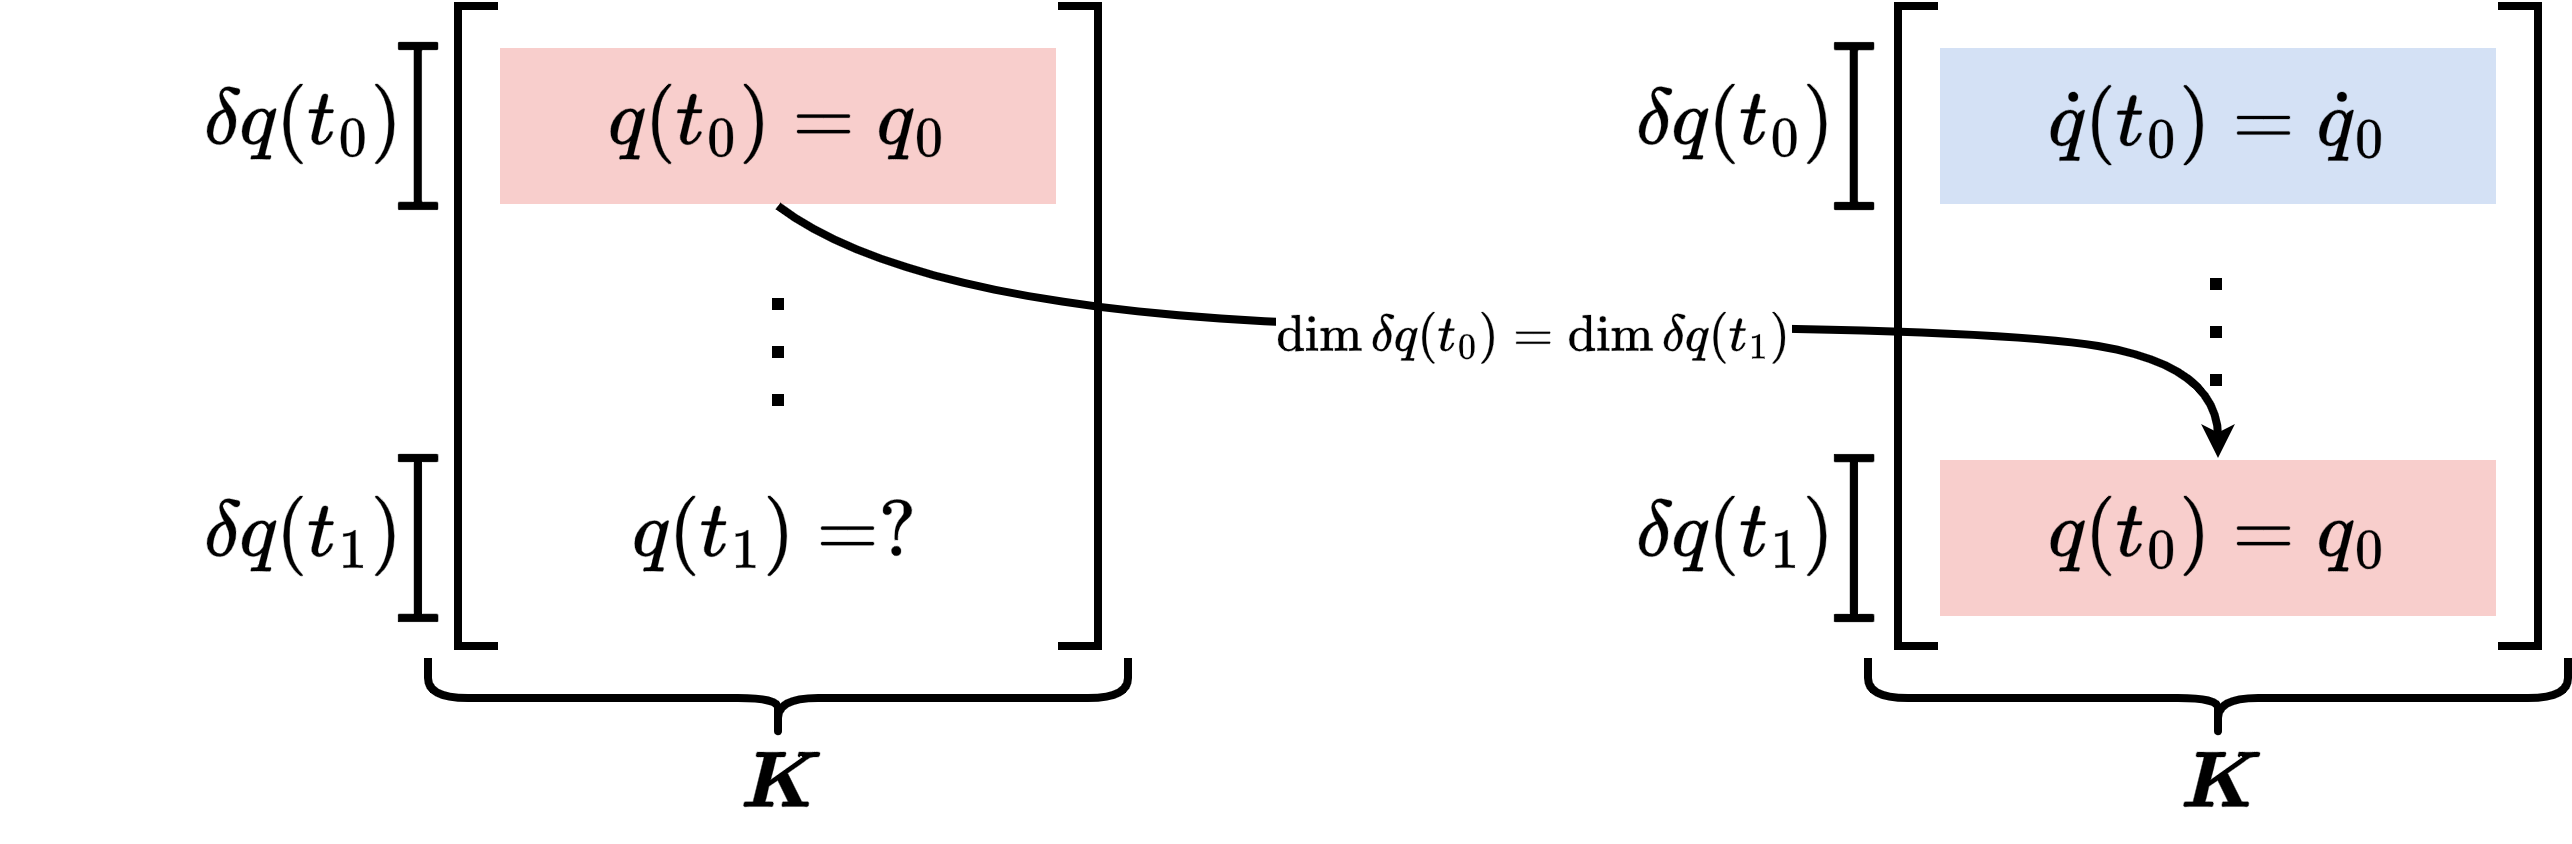
\includegraphics[scale=0.45]{fig/math/边界条件转移图.png}
\caption{\centering{初始时刻本质边界条件直接施加到时间末端}}
\label{fg:δq=q}
\end{figure}

同时，将初始时刻的本质边界条件直接施加到时间末端位置的方法会破坏刚度矩阵的对称性，从而导致下列问题：
首先是存储困难，对称矩阵可利用对称性仅存储上三角或下三角部分数据，大幅节省内存开销。
而边界条件的非自然转移会打破矩阵元素的对称分布，非对称矩阵需完整存储所有行和列的元素，
尤其在大规模多维问题中，数据存储量会翻倍，给内存资源带来巨大压力；
然后是计算效率低，数值求解中针对对称矩阵的优化算法可将计算复杂度从$O(n^3)$降低至$O(n^2)$\cite{golub2013matrix}，
而非对称矩阵无法适配此类高效算法，需采用通用矩阵求解方法，
运算步骤增多、迭代次数增加，且数据读写量增大，直接导致整体计算效率大幅下降。
最后是计算稳定性差，对称矩阵的特征值均为实数，且数值求解过程中误差传播具有可控性，
不易出现震荡或发散；非对称矩阵可能存在复数特征值，易引发数值振荡，
同时边界条件转移带来的 “时空错位” 会加剧误差累积，在长时间积分或复杂载荷作用下，
误差可能持续放大，最终导致计算结果失真甚至求解失败。
所以，建立时域末端虚位移本质边界条件的施加方案，
是发展适用于任意节点分布时空伽辽金无网格法的必要条件。

综上所述，有限元模拟动力问题的分析方法经历了从传统迭代方法到基于哈密顿原理的时空混合离散方法的演变。
这些方法的发展不仅提高了分析的效率和精度，还增强了模拟的稳定性。
但哈密顿原理在完全时空离散有限元法处理动力问题仍然存在这时间末端边界和无法任意使用局部加密等问题，
这些问题成为发展哈密顿原理计算动力系统数值分析方法的瓶颈。
为此，本文将系统研究完全时空离散有限法元计算动力系统问题，
探究哈密顿变分原理作有限元分析时的边界问题，
从而确定处理时间末端边界问题的必要条件。
同时，建立一个在有限元伽辽金数值计算中能完全时空混合离散的方案。
从而得到更高效、精确的数值分析方法，从而能稳定应用到解决弹性波问题当中，
为有限元模拟弹性波检测技术应用提供可靠精确的数值分析工具。

\section{拉格朗日乘子型时域未端本质边界条件施加方案}

为解决基于哈密顿原理的传统有限元法在时间末端边界的问题，
本节提出一种基于拉格朗日乘子型的时域未端本质边界条件施加方案。
在上节中已知，试函数空间$\mathcal{Q}$和权函数空间$\mathcal{P}$不一致将会导致刚度矩阵不为方阵，无法求解。
本文所提方案是通过引入一个拉格朗日乘数$p$来代替原来无法数值实现的虚位移$\delta q$，现将试函数空间投影到$\mathcal{Q}'$空间中。
$\mathcal{Q}'$空间定义为：
\begin{equation}
\mathcal{Q}' = \left \{ q \in \mathcal{Q} \left \lvert \int_{t_0}^{t_1} \dot p m \dot q - p k q dt = pm\dot q \vert_{t=t_0}, \; \forall \delta p \in \mathcal{P} \right . \right \}
\end{equation}
随后，在$Q$空间中寻找使用作用量$\Phi$取最小值时的$q$。此时全新的能量泛函可表示为：
\begin{equation}\label{2.16}
\bar \Phi(q,p) = \Phi(q) - \int_{t_0}^{t_1} (\dot q m \dot p - q k p) dt + \dot q m p\vert_{t=t_0}
\end{equation}
对上式进行变分得到对应的弱形式：
\begin{multline}\label{delat Phi(u,p)}
    \delta \bar \Phi(q,p) = \delta \Phi(q) - \int_{t_0}^{t_1} (\delta \dot q m \dot p - \delta q k p) dt - \int_{t_0}^{t_1} (\delta \dot p m \dot q - \delta p k q) dt \\
    + \delta \dot q m p \vert_{t=t_0} + \delta p m \dot q \vert_{t=t_0} = 0
\end{multline}
引入相同节点的有限元近似同时离散$q$和$p$，整理可得如下伽辽金弱形式：
找到一组解$(q^h,p^h) \in \mathcal{Q}^h \times \mathcal{P}^h$，使得
\begin{equation}
    \begin{aligned}
        \int_{t_0}^{t_1} (\delta \dot q m \dot q - \delta q k q) dt - \int_{t_0}^{t_1} (\delta \dot q m \dot p - \delta q k p) dt &= 0, \quad & \forall \delta q^h \in \mathcal{Q}^h \\
        - \int_{t_0}^{t_1} (\delta \dot p m \dot q - \delta p k q) dt &= - \delta p m  \dot q \vert_{t=t_0}, \quad & \forall \delta p^h \in \mathcal{P}^h
    \end{aligned}
\end{equation}

为了验证引入拉格朗日乘子后的双变量弱形式与原有强形式控制方程之间的等价性，
对上述弱形式方程做分部积分。对于关于虚位移$\delta q$部分的变分方程进行分部积分可得：
\begin{equation}
    \begin{aligned}
        & - \int_{t_0}^{t_1} \delta q (m\ddot q + k q ) dt + \delta q m \dot q \vert_{t_0}^{t_1}
        + \int_{t_0}^{t_1} \delta q (m\ddot p + k p ) dt - \delta q m \dot p \vert_{t_0}^{t_1} = 0
    \end{aligned}
\end{equation}
整理得到：
\begin{equation}
    - \int_{t_0}^{t_1} \delta q \left( (m\ddot q + k q ) - (m\ddot p + k p ) \right) dt + \delta q m (\dot q - \dot p)\vert_{t_0}^{t_1} = 0
\end{equation}
同理，对关于拉格朗日乘子变分$\delta p$的方程进行分部积分：
\begin{equation}
    \int_{t_0}^{t_1} \delta p (m\ddot q + k q ) dt - \delta p m \dot q \vert_{t_0}^{t_1} = - \delta p m \dot q \vert_{t=t_0}
\end{equation}
结合边界初始项对应，整理化简为：
\begin{equation}
    \int_{t_0}^{t_1} \delta p (m\ddot q + k q ) dt - \delta p m \dot q \vert_{t=t_0} = 0
\end{equation}

根据哈密顿原理，虚位移$\delta q$在时间端点处为零，且在位移边界条件处也必须为零。
最终，哈密顿原理\eqref{delat Phi(u,p)}所应用的欧拉-拉格朗日方程强形式为：
\begin{equation}
    \left \{
    \begin{aligned}
        & m\ddot q + k q = 0, \\
        & m\ddot p + k p = 0,  \\
        & \dot p \vert_{t=t_0} = \dot q \vert_{t=t_0}, \\
        & \dot p \vert_{t=t_1} = \dot q \vert_{t=t_1}, \\
        & \dot q \vert_{t=t_0} = \dot q_0
    \end{aligned}
    \right .
\end{equation}

通过有限元近似表达式\eqref{q_h}和\eqref{dotq_h}，
对广义变量$q$和拉格朗日乘数$p$以及他们对时间的一阶导数进行有限元近似，
可得对应的离散控制方程为：
\begin{equation}
\begin{bmatrix}
\boldsymbol K & -\boldsymbol K \\ -\boldsymbol K & \boldsymbol 0
\end{bmatrix}
\begin{Bmatrix}
\boldsymbol q \\ \boldsymbol p
\end{Bmatrix} =
\begin{Bmatrix}
 \boldsymbol 0 \\ -\boldsymbol f
\end{Bmatrix}
\end{equation}
其中，刚度矩阵$\boldsymbol K$和力向量$\boldsymbol f$的分量$K_{IJ}$和$f_I$与式\eqref{K_IJ}，\eqref{f_I}相同。
从上式可以看出，试函数空间和权函数空间均属于相同的离散空间，$\mathcal{Q}^h\times \mathcal{P}^h$。
在施加强制边界条件时，将不再出现由于空间不匹配造成施加困难的问题。本文采用罚函数法\cite{hughes2000finite}对$q$和$p$相关的本质边界条件进行施加。
罚函数的增广能量泛函可写为：
\begin{equation}
\tilde{\Phi}(q,p)
= \bar \Phi(q,p)
+ \frac{\alpha}{2}\left(q \vert_{t=t_0}-q_0\right)^2
+ \frac{\beta}{2}\left(p\vert_{t=t_1}-\bar p_1\right)^2
\end{equation}
其中，$\alpha$和$\beta$分别为与$q$、$p$相关本质边界条件的罚参数，
$q_0$为初始时刻位移边界值，$\bar p_1$为时间末端动量边界目标值。
对上式变分可得附加边界项：
\begin{equation}
\delta \tilde{\Phi} -\delta \bar \Phi
= \alpha \left(q\vert_{t=t_0}-q_0\right)\delta q\vert_{t=t_0}
+ \beta \left(p\vert_{t=t_1}-\bar p_1\right)\delta p\vert_{t=t_1}
\end{equation}
罚参数取值应足够大以保证边界约束近似满足，同时避免过大导致离散方程病态，
通常可按问题特征刚度量级进行比例选取并结合条件数进行校核。
相对应的离散控制方程可表示为：
\begin{equation}\label{2.25}
\begin{bmatrix}
\boldsymbol K + \boldsymbol K^\alpha & -\boldsymbol K \\ -\boldsymbol K & \boldsymbol K^\beta
\end{bmatrix}
\begin{Bmatrix}
\boldsymbol q \\ \boldsymbol p
\end{Bmatrix} =
\begin{Bmatrix}
 \boldsymbol f^\alpha \\ -\boldsymbol f + \boldsymbol f^\beta
\end{Bmatrix}
\end{equation}
其中，$\boldsymbol K^\alpha$和$\boldsymbol f^\alpha$、
$\boldsymbol K^\beta$和$\boldsymbol f^\beta$
分别为施加与$q$和$p$相关的本质边界条件刚度矩阵和力向量，分量表达式如下：
\begin{align}
K^\alpha_{IJ} &= \alpha N_I N_J |_{t=t_0} \quad
f^\alpha_I = \alpha N_I q_0 |_{t=t_0} \label{2.26} \\
K^\beta_{IJ} &= \beta N_I N_J |_{t=t_1} \quad
f^\beta_I = \beta N_I \bar p_1 |_{t=t_1} \label{2.27} \\
\end{align}
式中$\alpha$为用于施加与广义位移$q$相关的本质边界条件的罚函数因子，
$\beta$为用于施加与广义动量$p$相关的本质边界条件的罚函数因子。

综上所述，由于在使用哈密顿原理计算动力问题时要求弱形式在时间末端的虚位移等于零，
才能等价于强形式，但这种方式无法数值实现。
所以，我们通过引入一个拉格朗日乘数$p$代替原来无法数值实现的虚位移$\delta q$，
构造出一个关于$q$和$p$的双变量的弱形式，
再将这个弱形式作为一个投影项加入到原来的能量泛函式里进行变分计算，
最后通过有限元形函数近似得到对应的刚度矩阵和力向量，组装离散控制方程进行代数求解。
这样，就解决了基于哈密顿原理的完全弱形式求解在时间末端边界条件的问题，
为时空有限元法解决动力学问题提供有力的理论支撑。









\section{数值算例}
\subsection{无阻尼弹簧小车问题}\label{ch:wznthxc}

考虑一维弹簧小车问题，如图\ref{fg:2.3}所示，一辆质量为$m = 1.0$的小车，
在初始位移$q_0=1.0$和初始速度$\dot q_0=1.0$作用下水平向右移动。
同时，一个刚度系数为$k=50$的弹簧作用在小车的左端，
整个弹簧小车模型的左端为固定支座，右端不施加任何约束。
现取总时间$T=8$，计算时间步长分别为$0.25,0.125,0.0625$和$0.03125$情况下的运动状态。

根据弹性力学的分析，该弹簧小车问题的解析解为：
\begin{equation}\label{2.28}
\begin{split}
q(t) &= q_0 \cos (\omega t) + \frac{\dot q}{\omega} \sin(\omega t) \\
\omega &= \sqrt{\frac{k}{m}}
\end{split}
\end{equation}

通过控制方程我们可以采用Newmark-$\beta$法对它进行动力分析，
根据式\ref{newmark-explicit}-\ref{newmark-semi-implicit}
所提到的在计算时，根据$\gamma$和$\beta$的取值不同，区分的三种迭代法进行测试。
最后根据Newmark-$\beta$法得到计算结果，
和我们所提出的基于拉格朗日变分方案的哈密顿法的计算结果作对比来测试方法的准确性。

弹簧小车的求解域分别通过图\ref{fg:bar}所示采用均布的四种疏密不同的节点进行计算，
其中节点个数$n=32-256$分别对应$\Delta t=0.25-0.03125$的时间步长。

首先对弹簧小车问题在不同计算方法和不同的时间步长下的位移随时间变化对比图进行了分析，
图\ref{fg:0.25}-\ref{fg:0.03125}为分析结果，
实线为精确的解析解和我们所提出的基于拉格朗日变分方案的计算结果，
虚线为$\gamma$和$\beta$在不同取值下的Newmark-$\beta$法位移随时间变化的计算结果。
其中灰色折线为$\gamma=0$、$\beta=0$时的显式格式，可以看出无论在何种时间步长的计算下，
该算法的计算稳定性最差，且计算所得的误差也是远远大于其他算法，计算精度很低。

绿色折线为$\gamma=1$、$\beta=\frac{1}{2}$时的隐式格式计算结果，
由于隐式算法对时间步长不敏感，所以计算结果相较于显式格式会稳定一些，
但是从图中可以看出隐式算法会出现严重的数值耗散现象，
导致数值结果被过度衰减，振荡逐渐趋近于停止。

蓝色折线为$\gamma=1$、$\beta=0$时的半隐式格式计算结果，
该方法的计算结果是明显优于前两种迭代法的。
因为半隐迭代方程满足哈密顿正则方程生成的保辛算法(Symplectic integrators)，\cite{GAGARINA2016370}
通过勒让德变换能等价于哈密顿正则方程，
在哈密顿正则方程的情况下迭代计算，角动量是守恒的，所以计算精度更高。
但是，该方法在强形式框架下，仍然难以完全避免数值弥散现象，
随着时间迭代步数的增加，数值解与精确解之间的相位差会逐渐累积，
影响计算精度，尤其在长时程动力分析中表现得更为明显。

而红色实线为本文所提出的基于哈密顿原理的完全弱形式，再通过拉格朗日乘子变分求解的方案，
通过对比发现红色实线是最贴近于黑色实线所代表的精确解的计算结果，且从误差图中可以看出误差是所有方法中最小的。
这表明该方法的计算精度和稳定性都比之前的三种Newmark-$\beta$迭代法更好，
误差远远小于传统迭代的计算方法。同时，因为该方法是通过伽辽金弱形式在全域上做并行计算，
不同于传统迭代法在计算过程依赖于上一步的计算结果，难以实现高度并行化，
该方法可以一次性将位移求解出来，计算效率更高。

根据上面四种时间步长计算得出的位移结果，我们可以得到如图\ref{fg:tanhuangxiaocheL2}所示的位移误差收敛图。
从图中可以看出，当我们波速取$\omega=\sqrt{50}$时，节点密度采取$32,64,128,256$四种形式，
来测试基于拉格朗日变分方案的哈密顿完全弱形式法的误差收敛率时，
可以得到$2.0$的位移误差收敛率，达到理论的误差收敛率，证明该方案是能够准确收敛的。



\begin{figure}[H]
    \centering
        \begin{tabular}{c}
            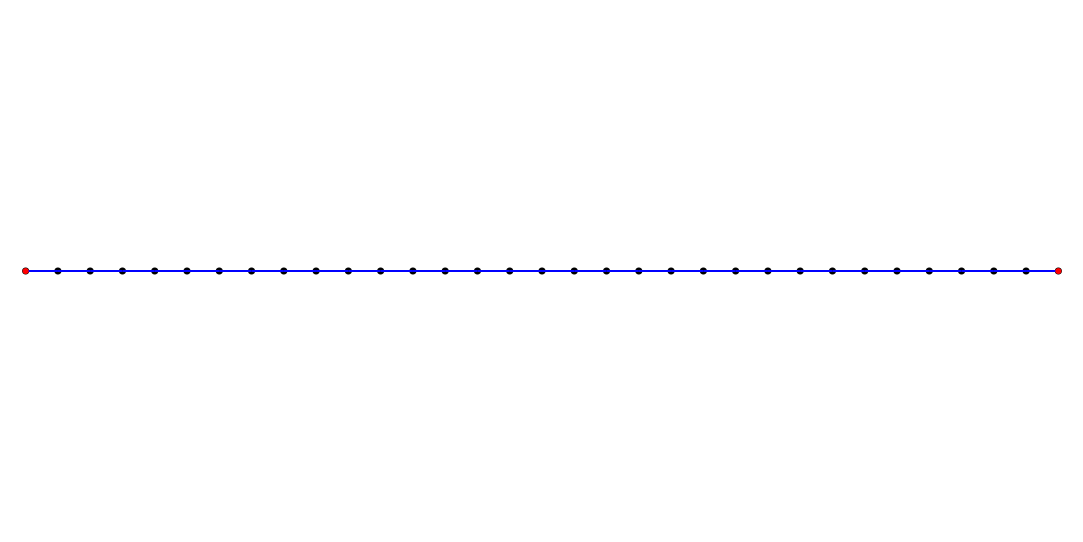
\includegraphics[width=0.8\textwidth]{fig/math/n=32.png} \\
            $n=32$ \\
            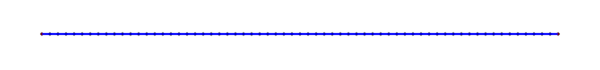
\includegraphics[width=0.8\textwidth]{fig/math/n=64.png} \\
            $n=64$ \\
            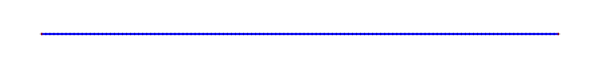
\includegraphics[width=0.8\textwidth]{fig/math/n=128.png} \\
            $n=128$ \\
            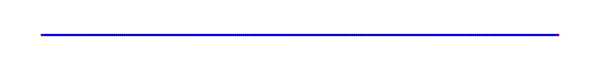
\includegraphics[width=0.8\textwidth]{fig/math/n=256.png} \\
            $n=256$
        \end{tabular}
        \caption{弹性小车问题节点均布布置示意图}\label{fg:bar}
\end{figure}

\begin{figure}[!h]
    \centering
        \begin{tabular}{c@{\hspace{15pt}}c}
            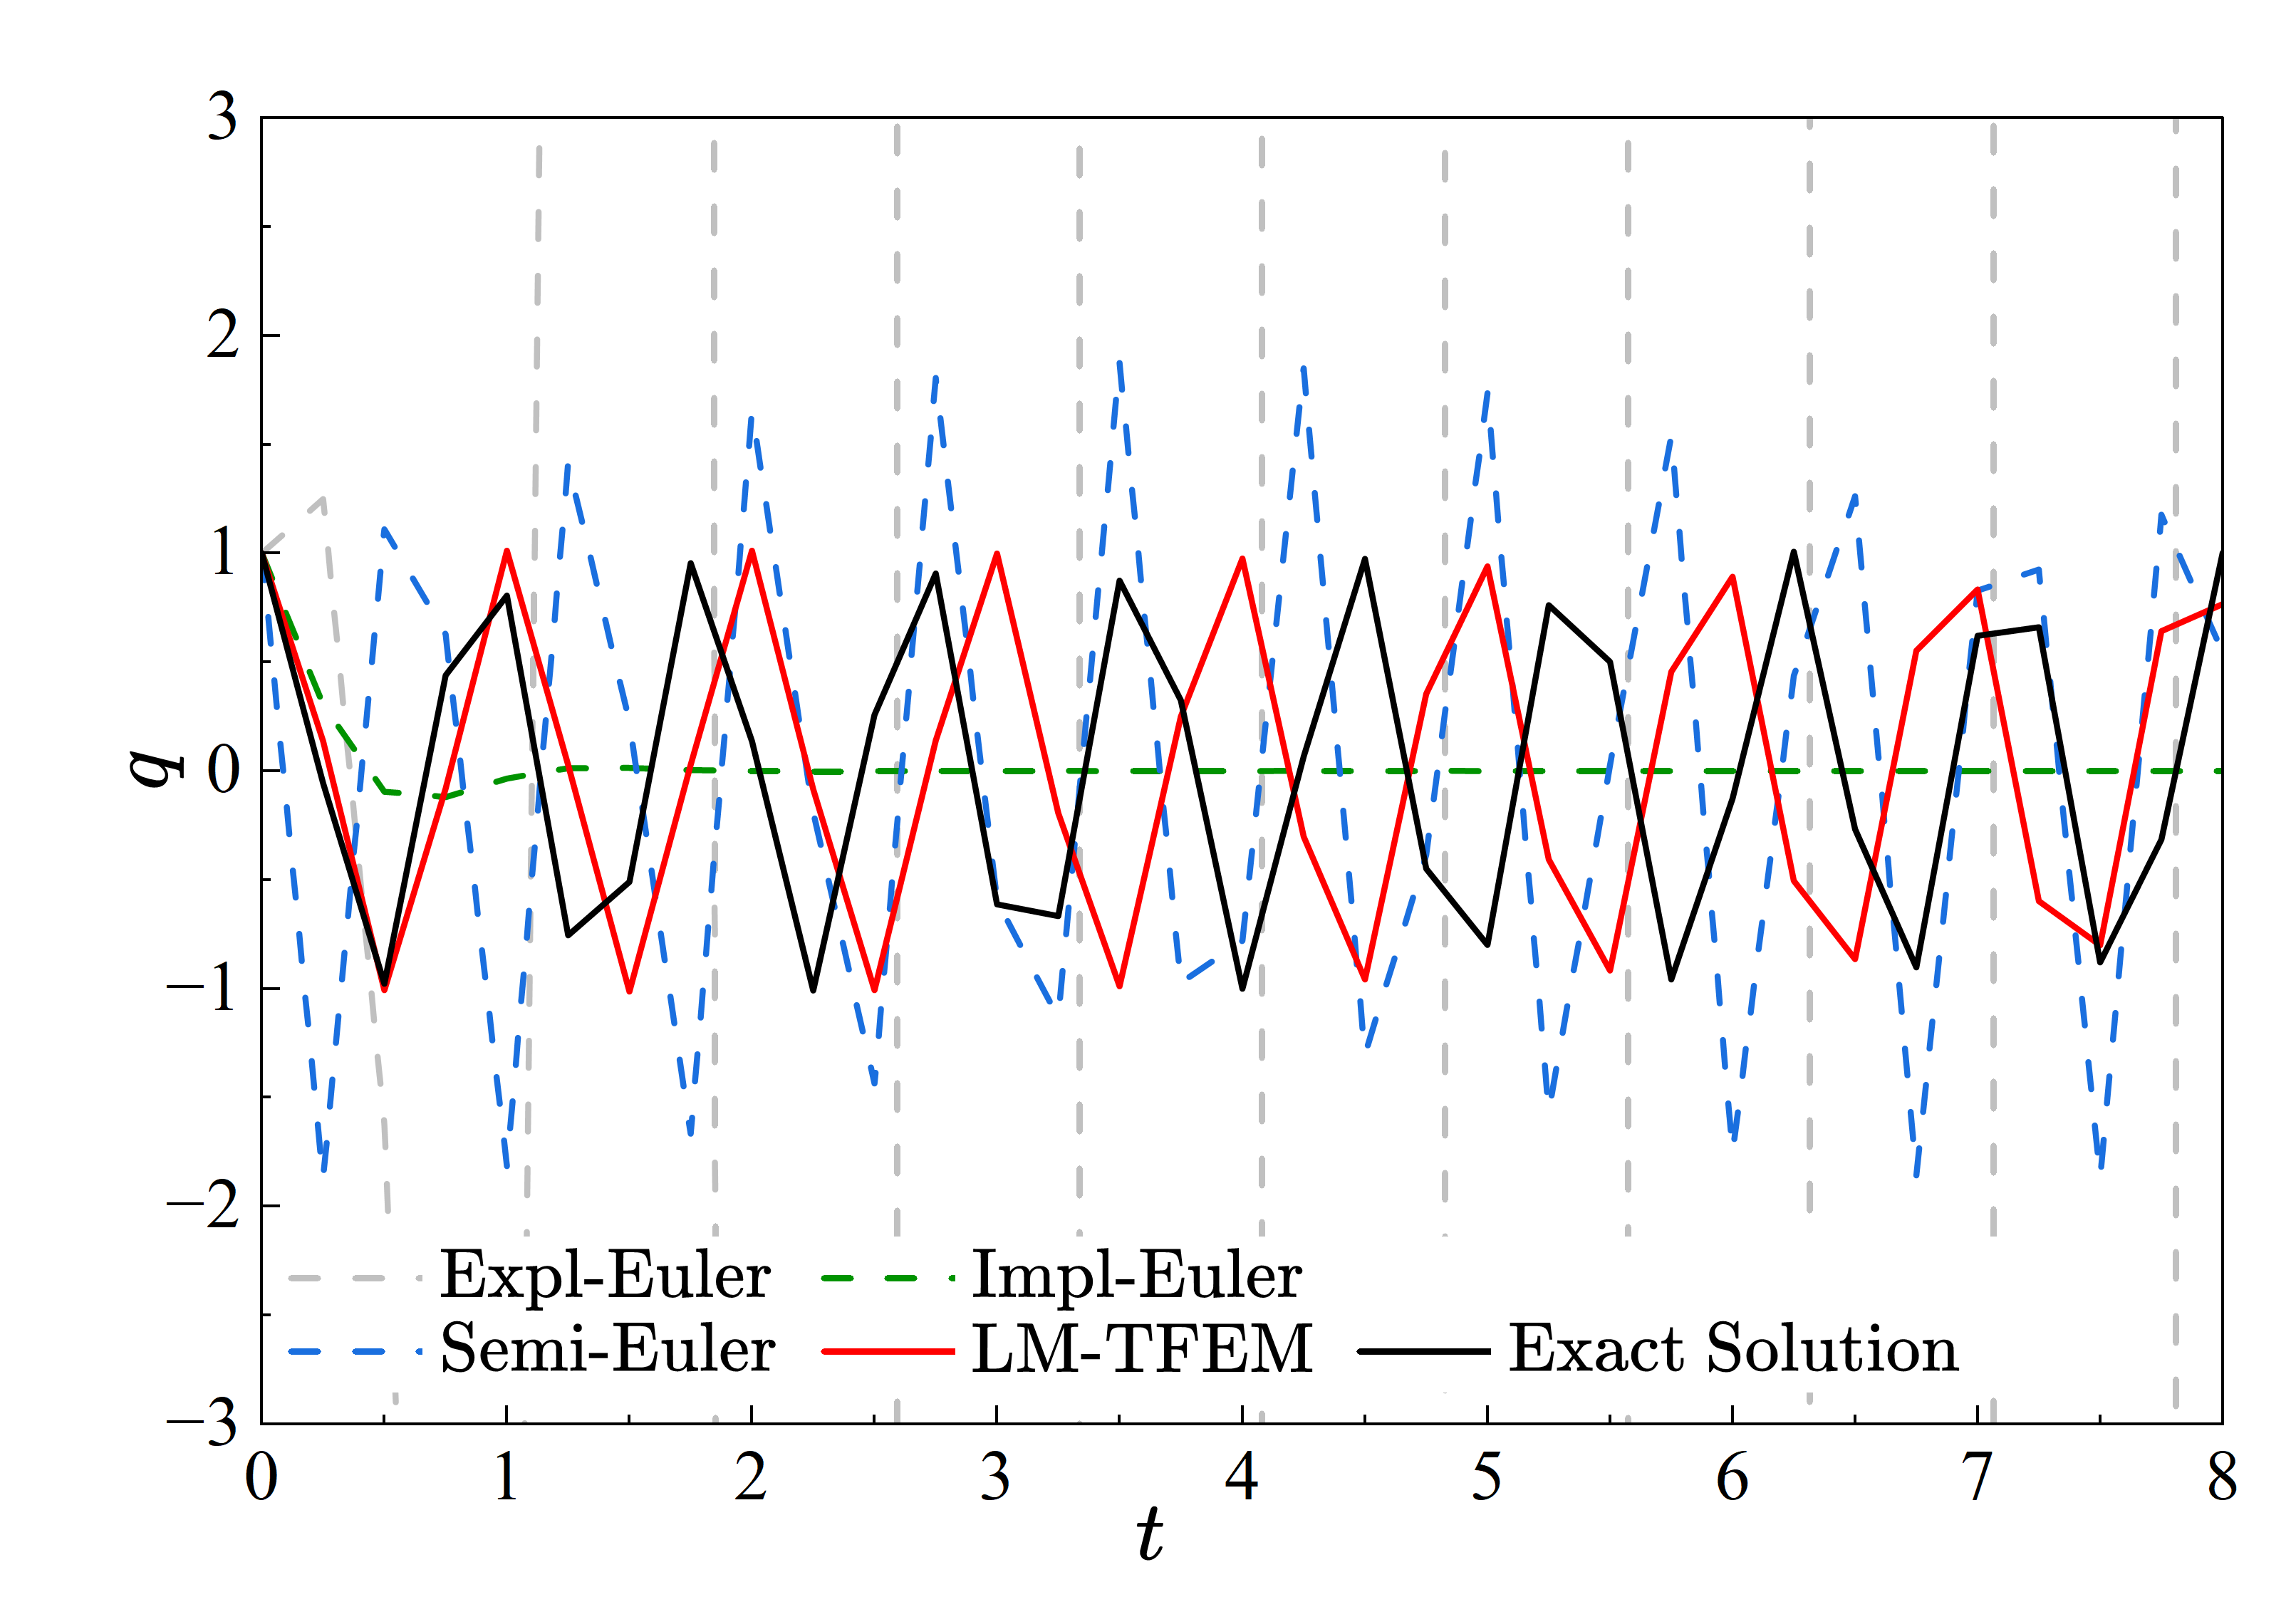
\includegraphics[width=0.45\textwidth]{fig/math/Δt=0.25位移图.png} &
            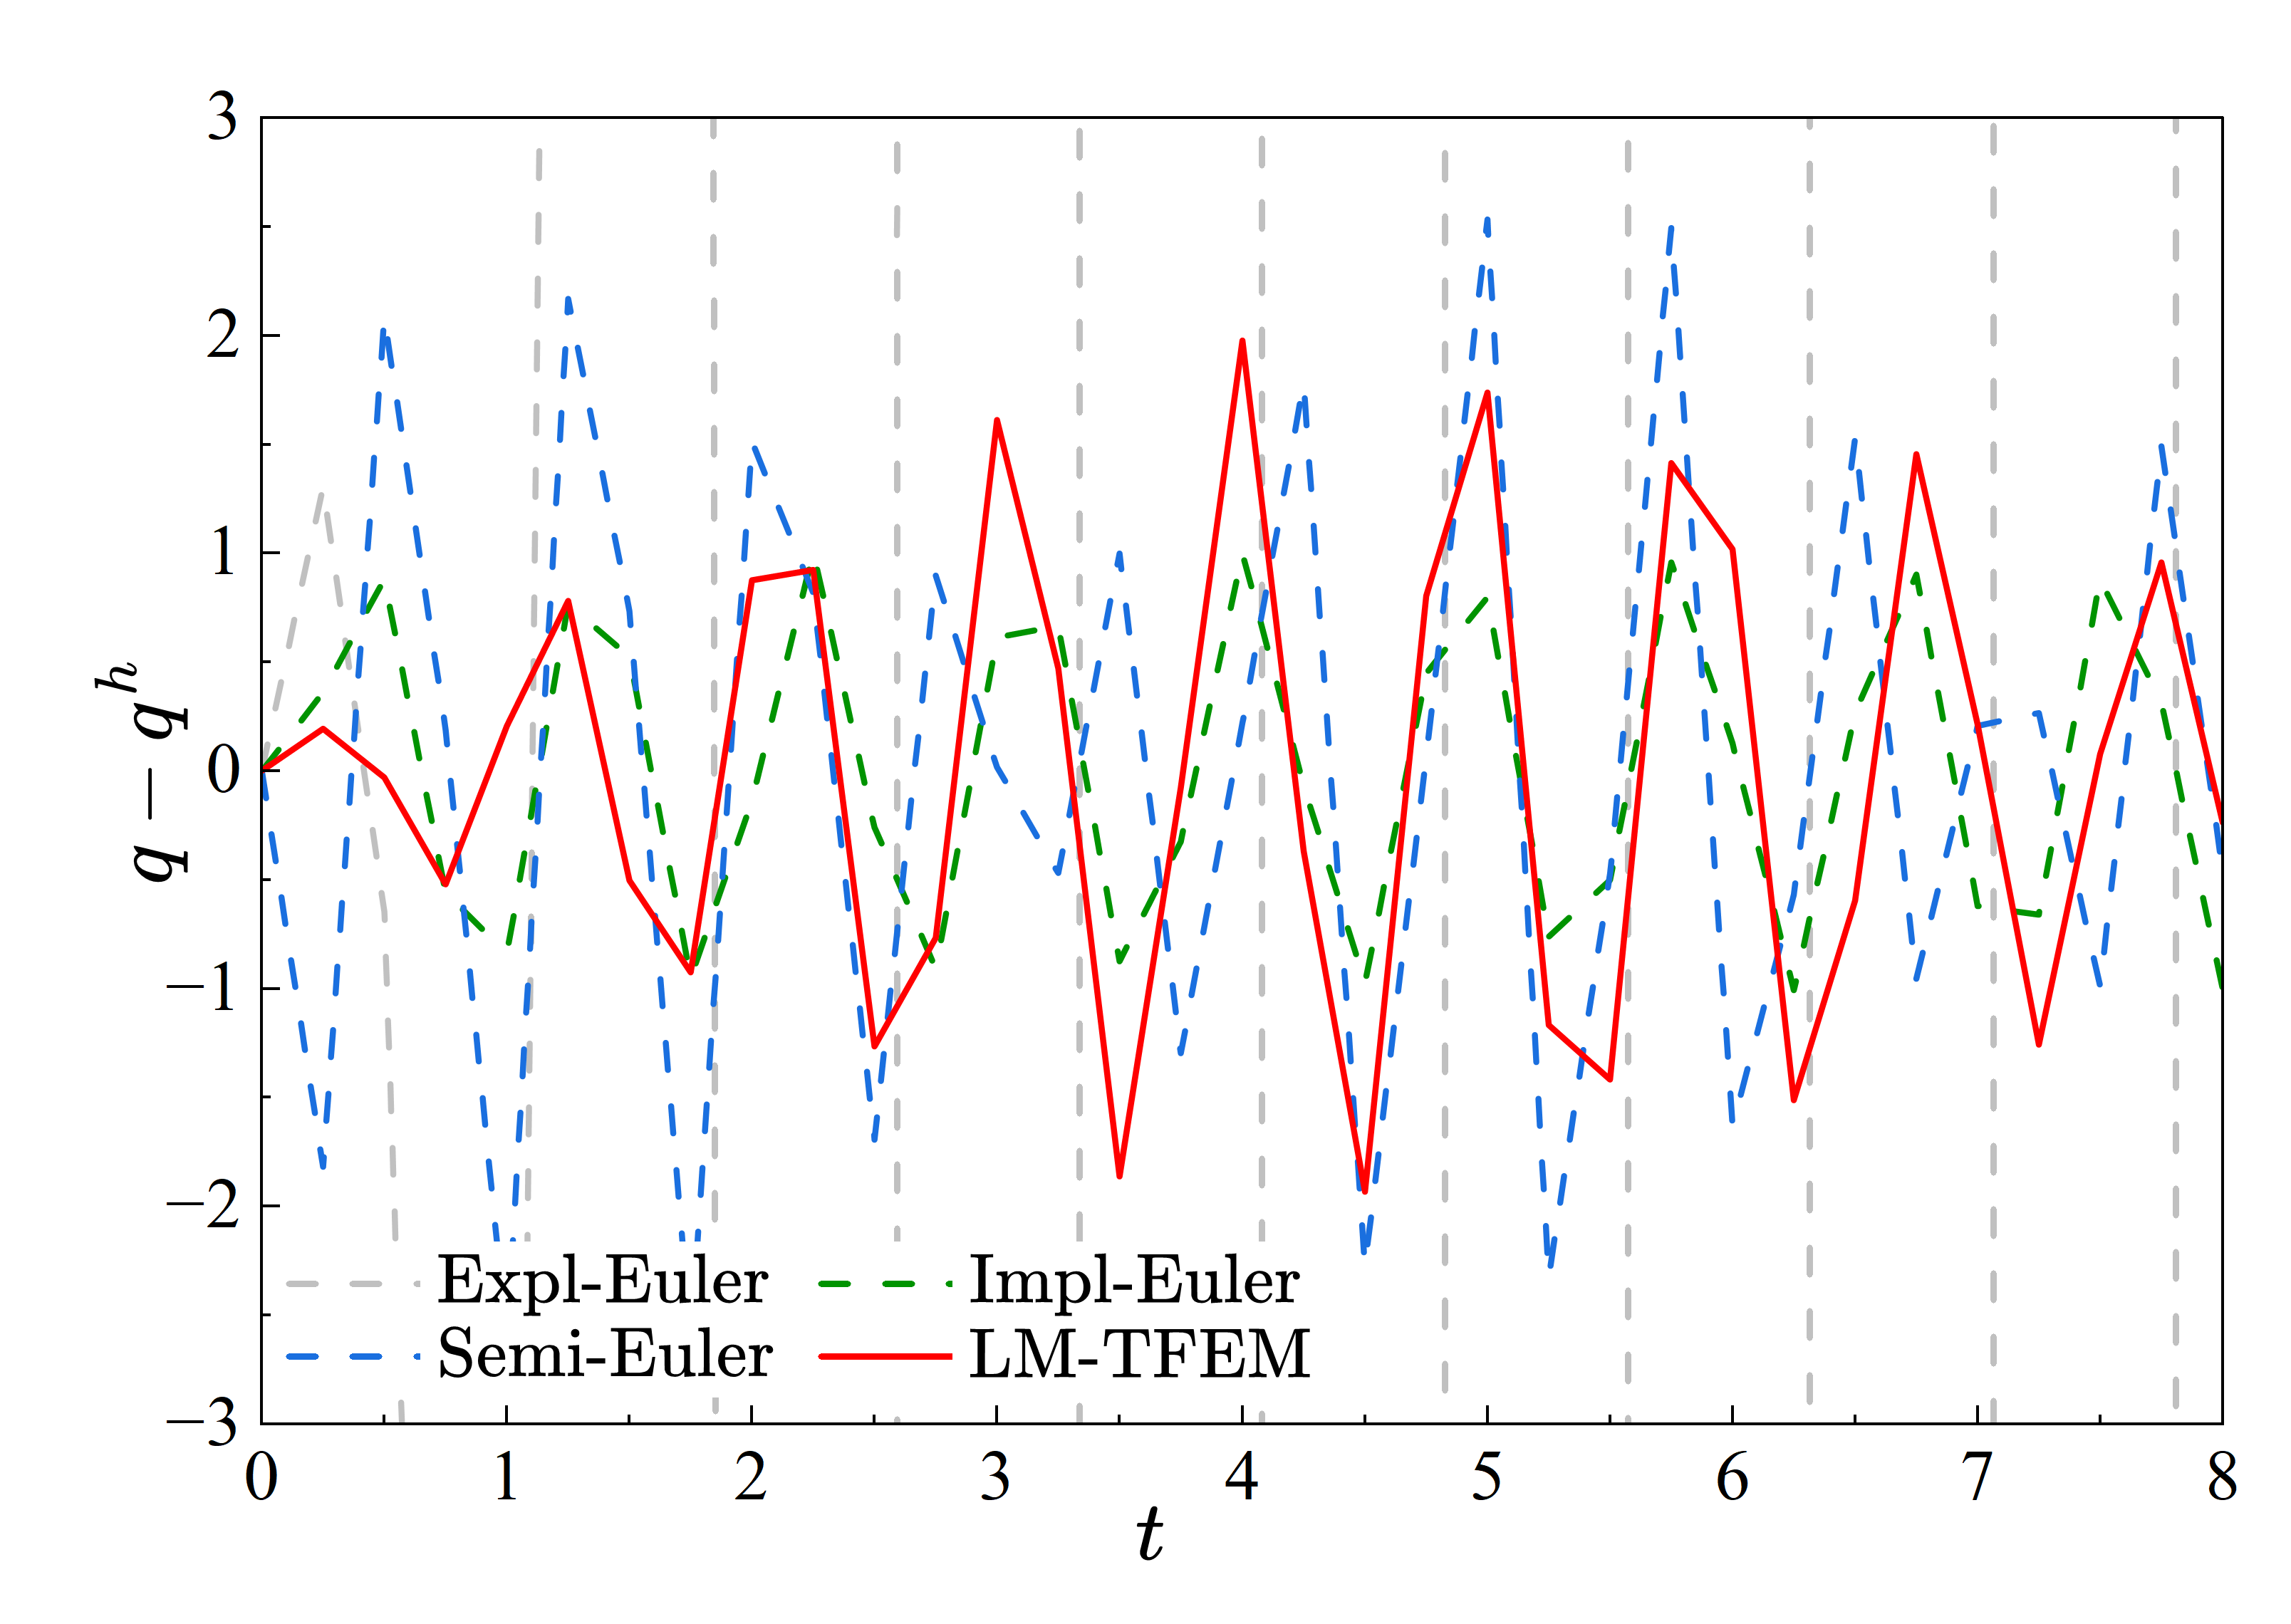
\includegraphics[width=0.45\textwidth]{fig/math/Δt=0.25位移误差图.png} \\
        \end{tabular}
        \caption{$\Delta t=0.25$时四种方法计算弹簧小车问题的位移图与误差图}\label{fg:0.25}
\end{figure}
\begin{figure}[!h]
    \centering
        \begin{tabular}{c@{\hspace{15pt}}c}
            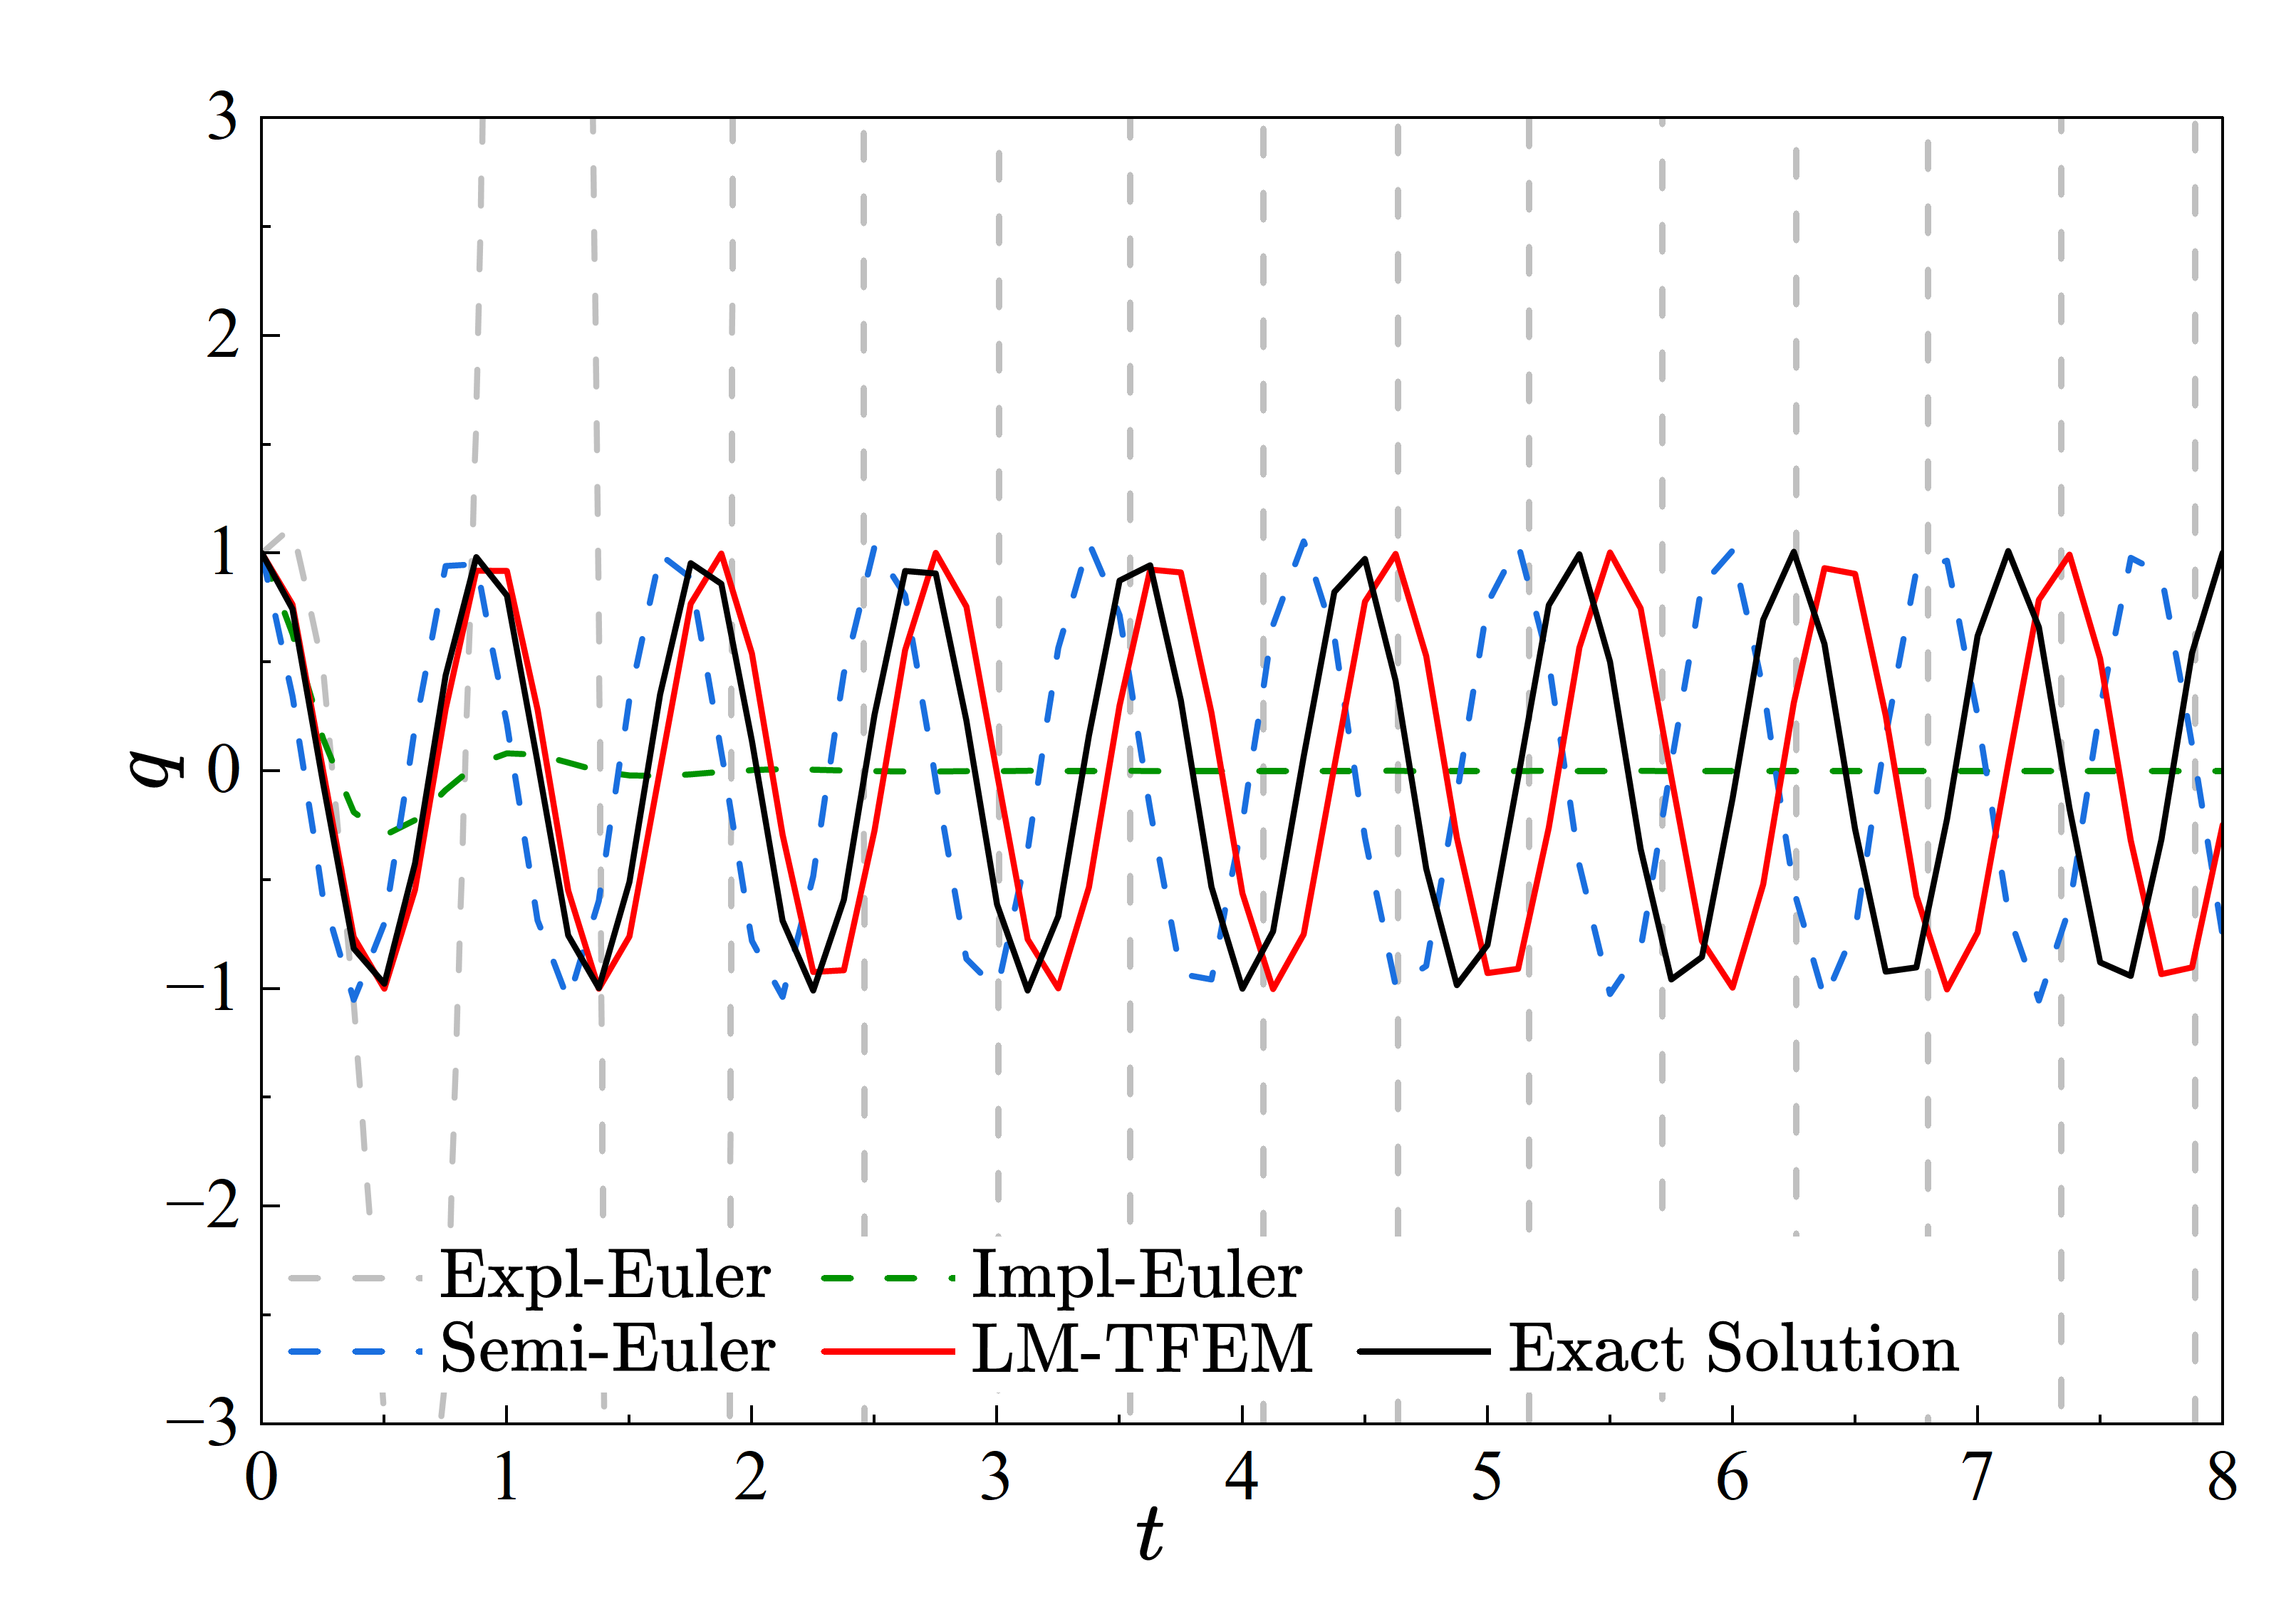
\includegraphics[width=0.45\textwidth]{fig/math/Δt=0.125位移图.png} &
            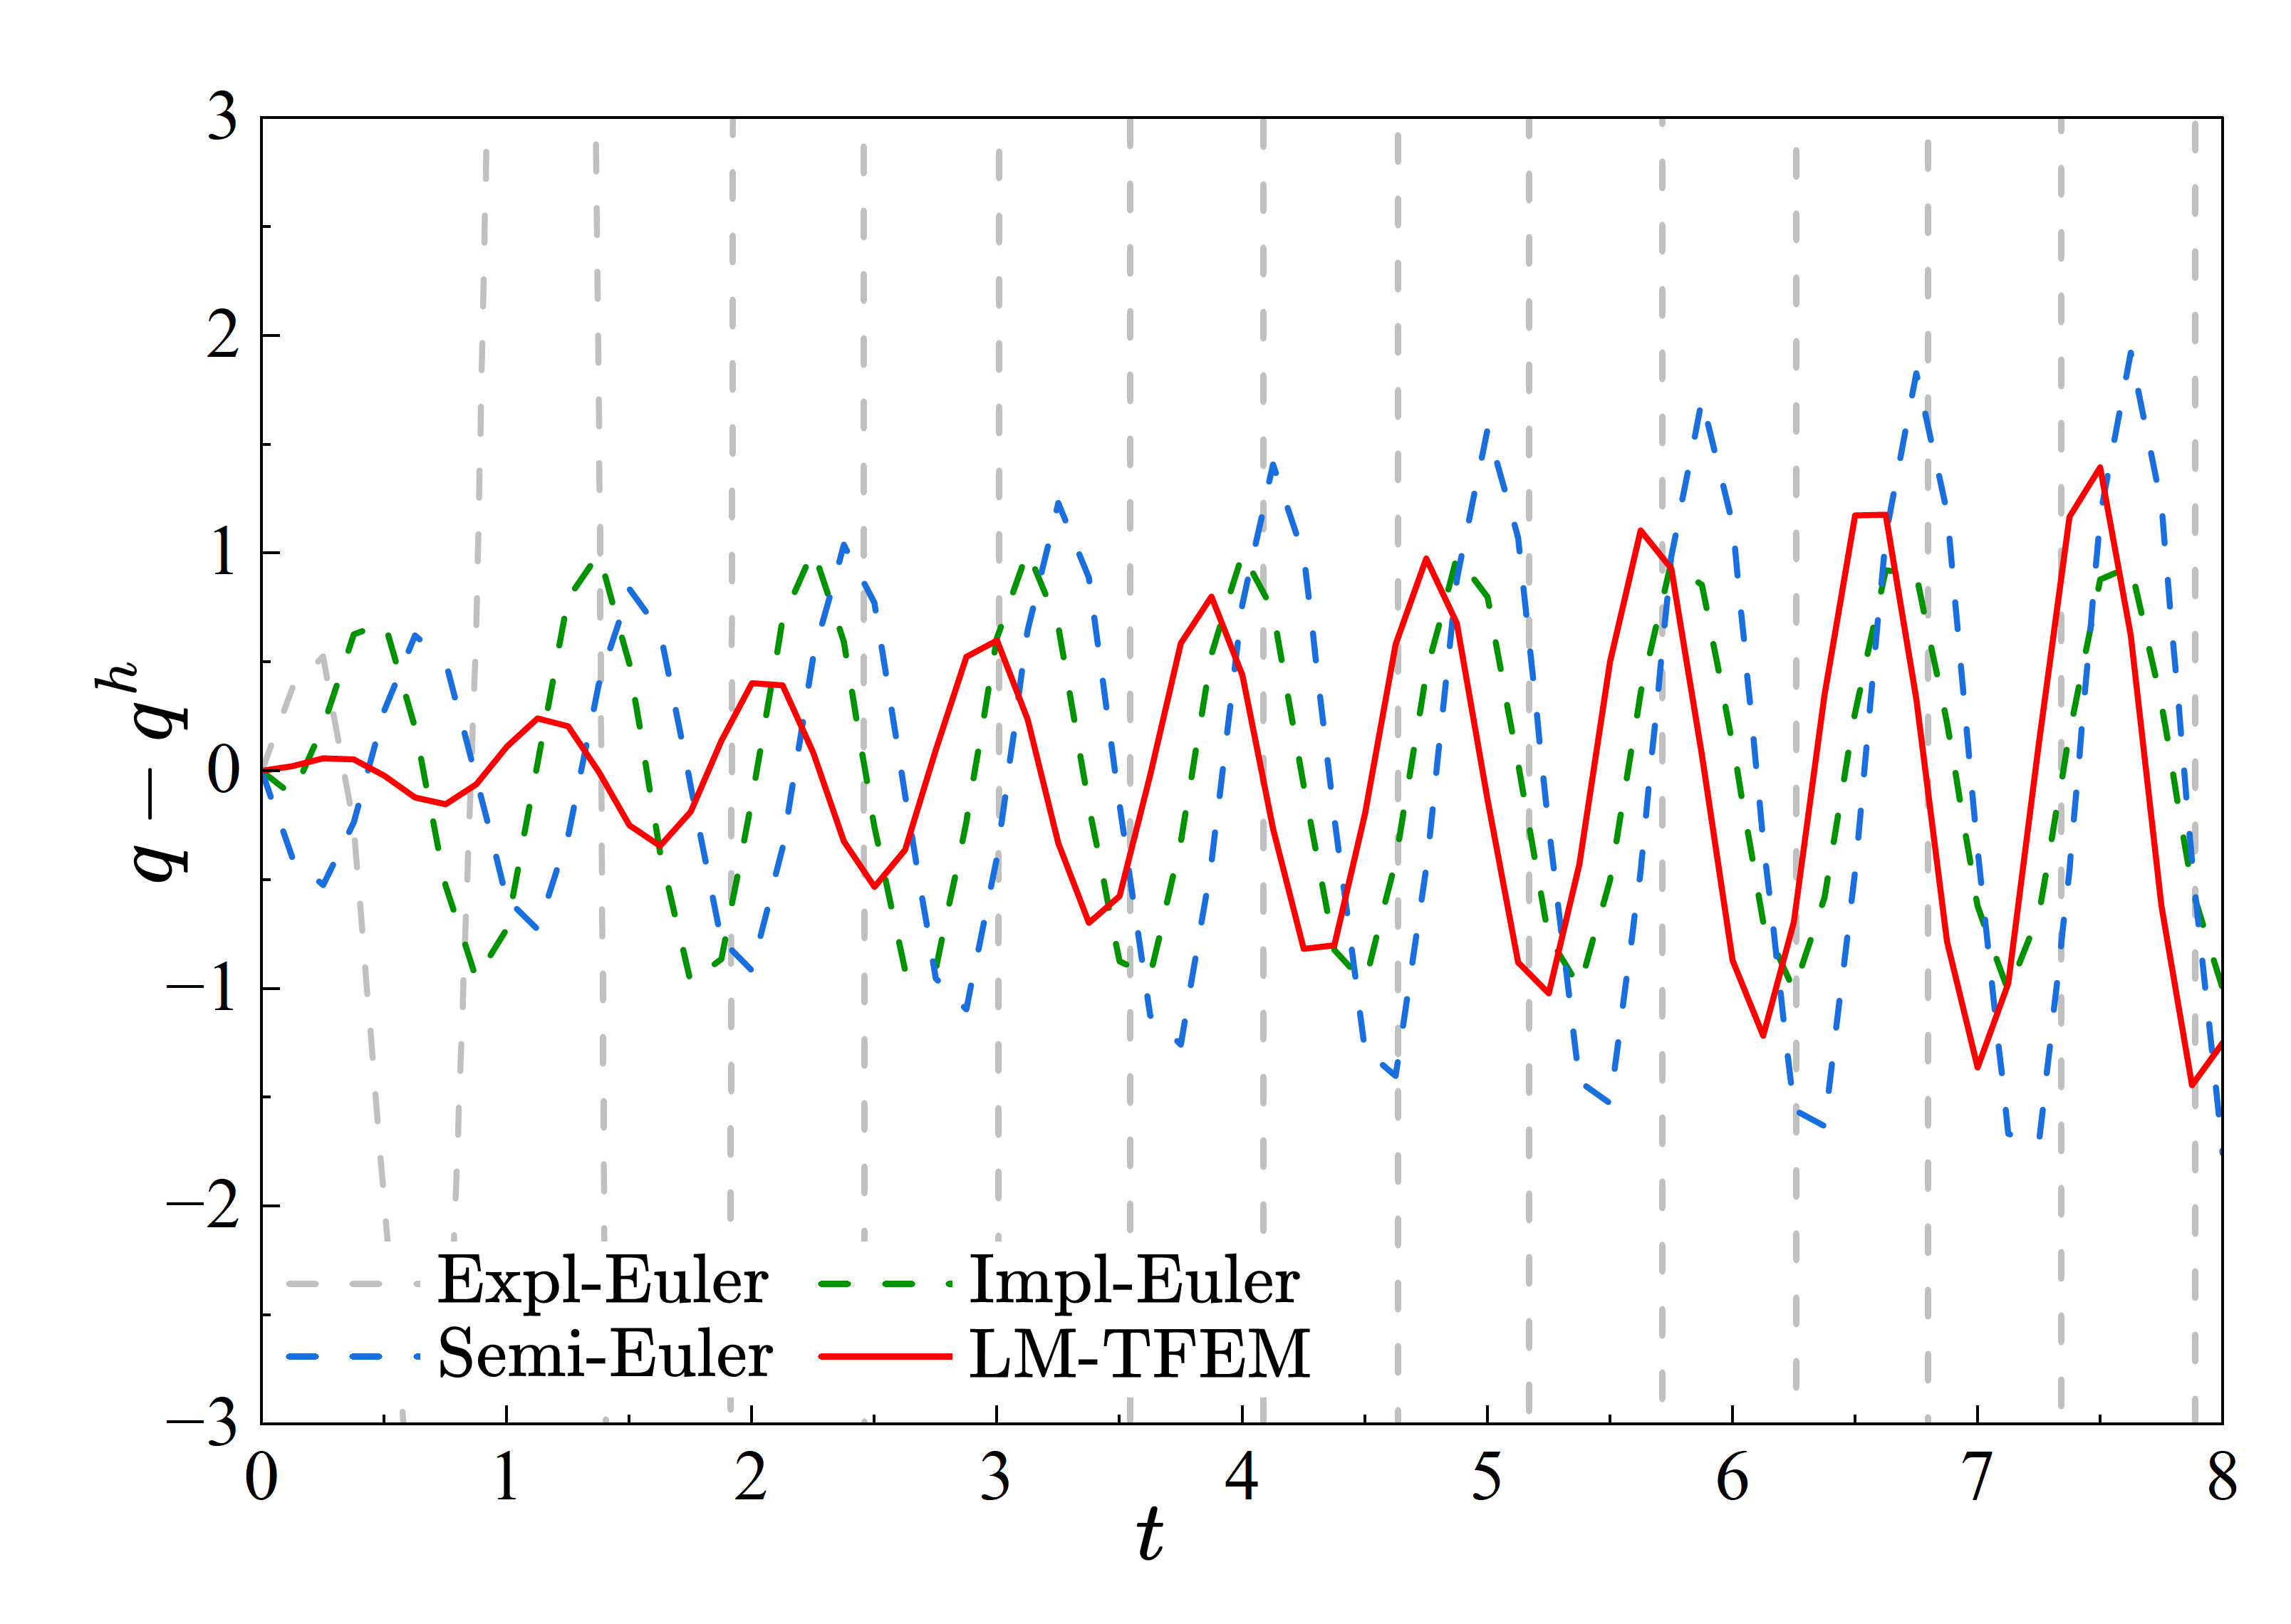
\includegraphics[width=0.45\textwidth]{fig/math/Δt=0.125位移误差图.png} \\
        \end{tabular}
        \caption{$\Delta t=0.125$时四种方法计算弹簧小车问题的位移图与误差图}\label{fg:0.125}
\end{figure}
\begin{figure}[!h]
    \centering
        \begin{tabular}{c@{\hspace{15pt}}c}
            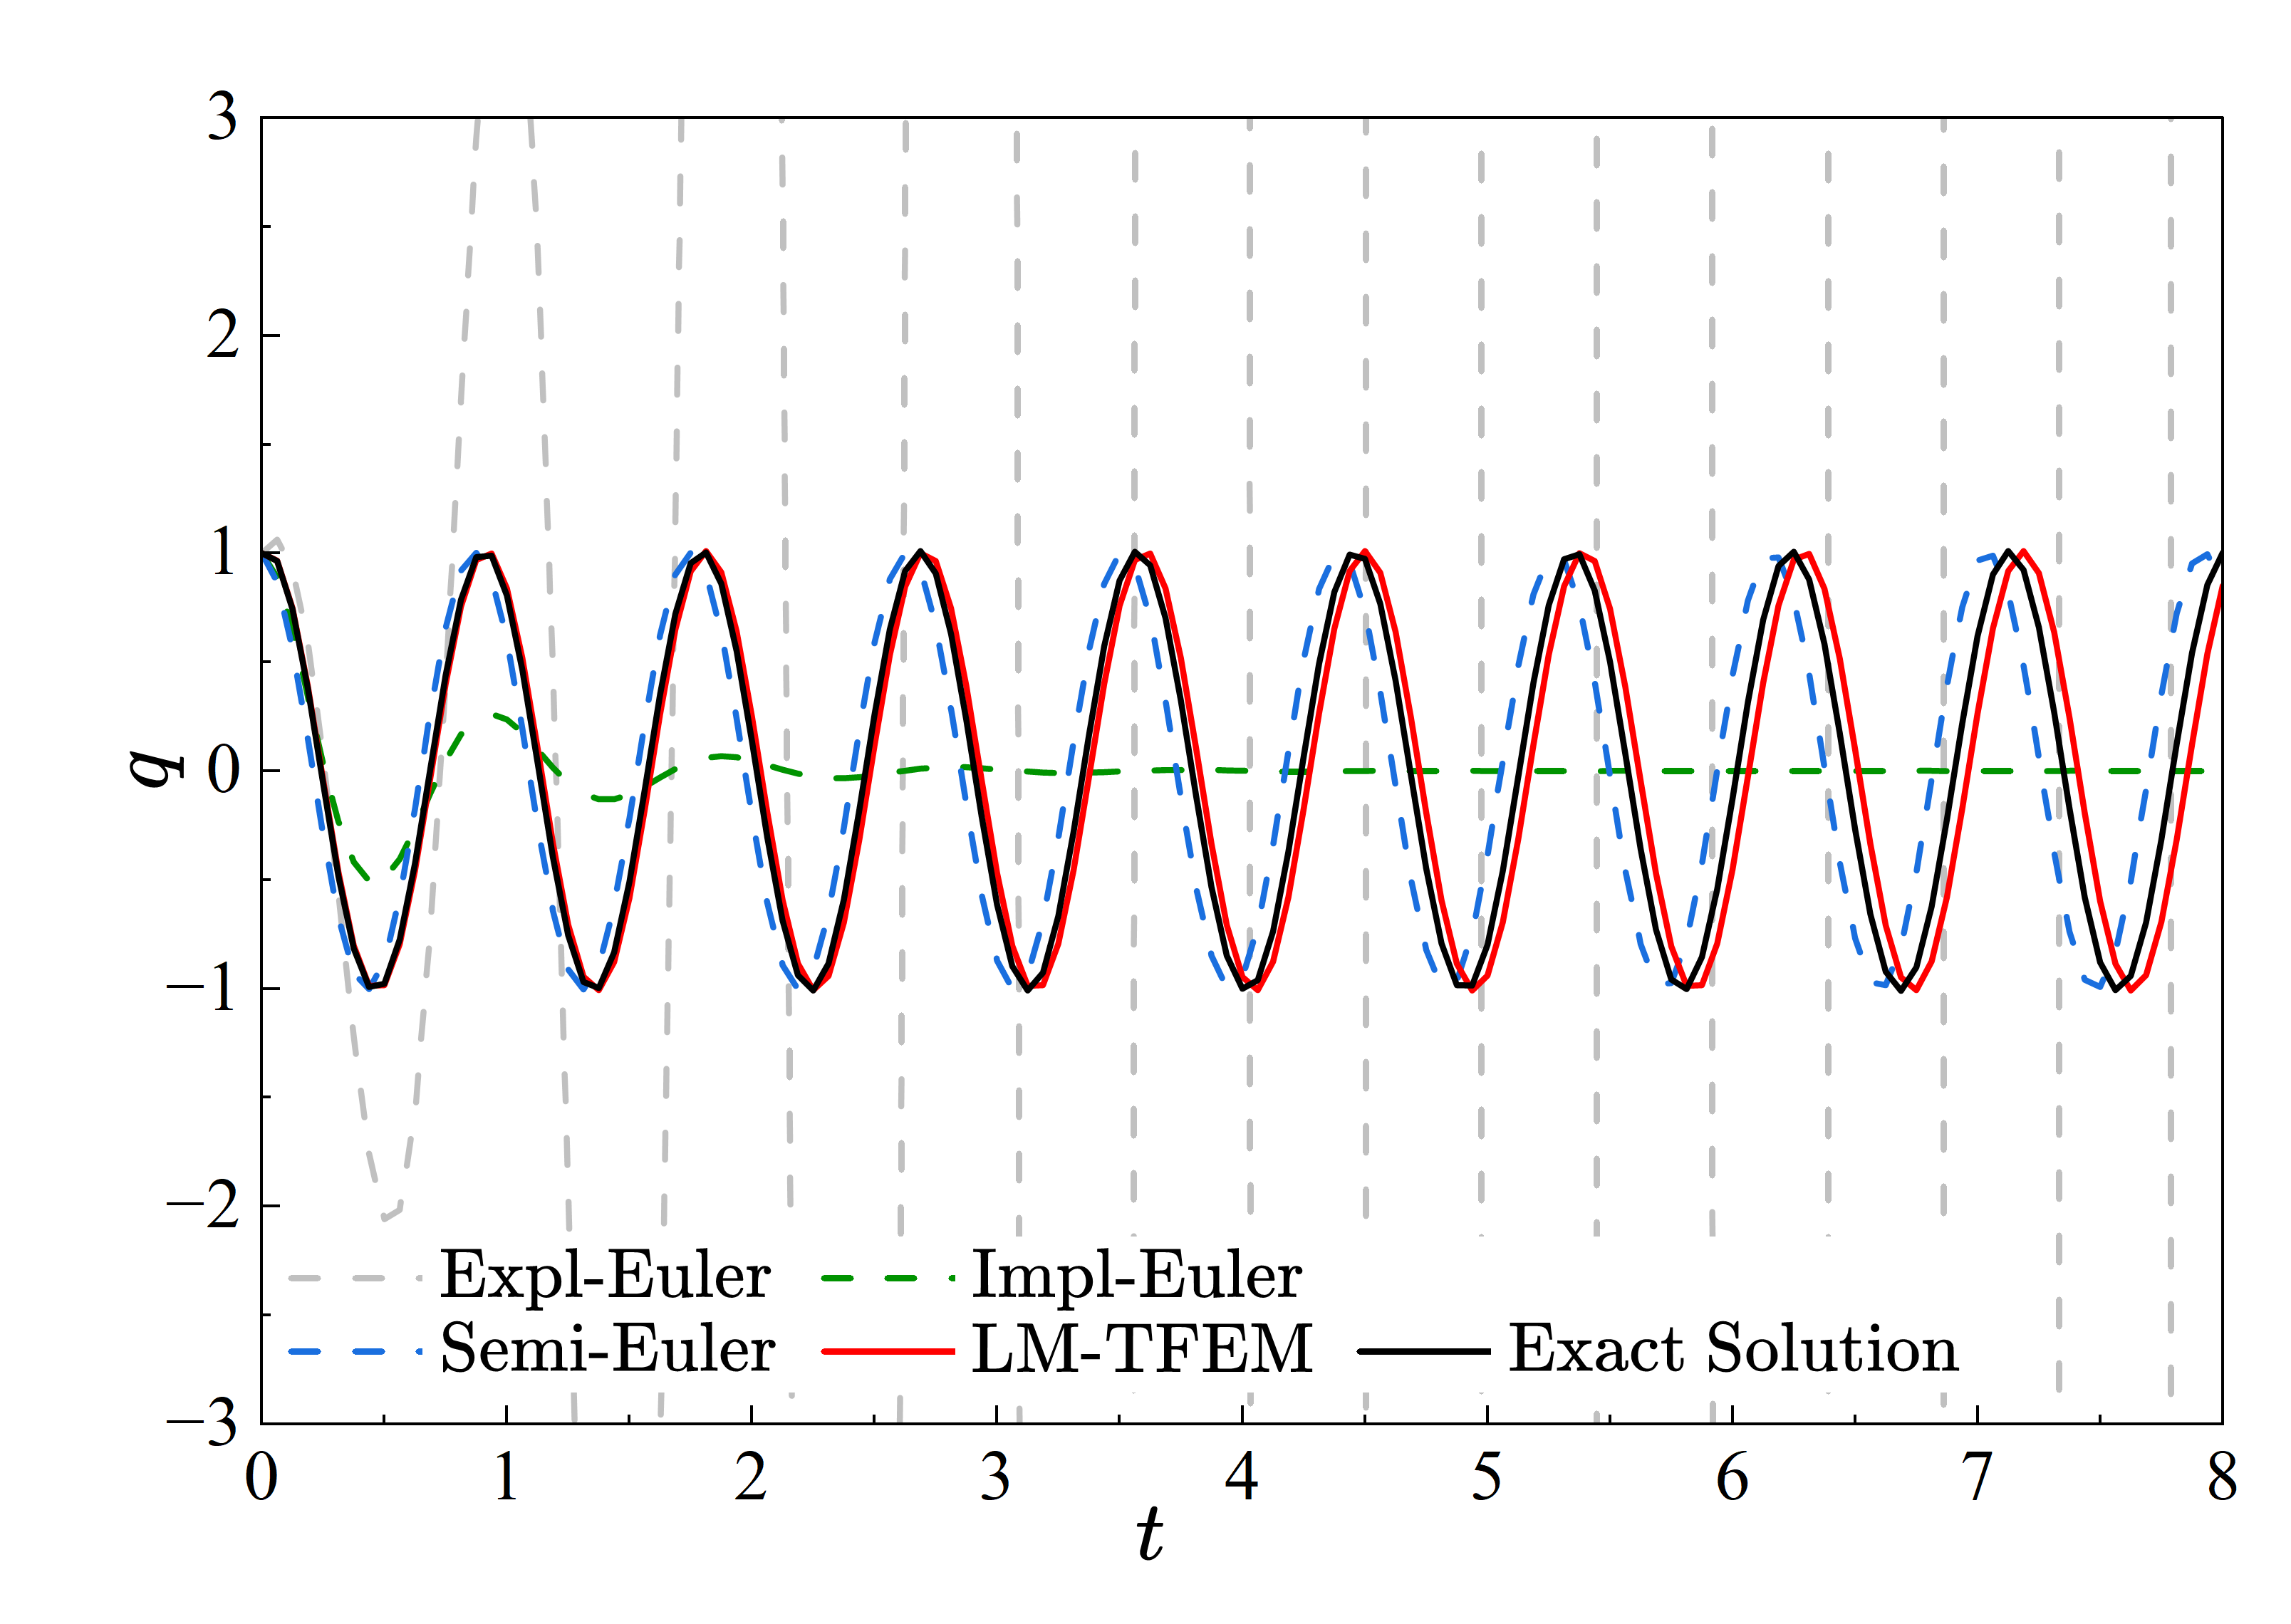
\includegraphics[width=0.45\textwidth]{fig/math/Δt=0.0625位移图.png} &
            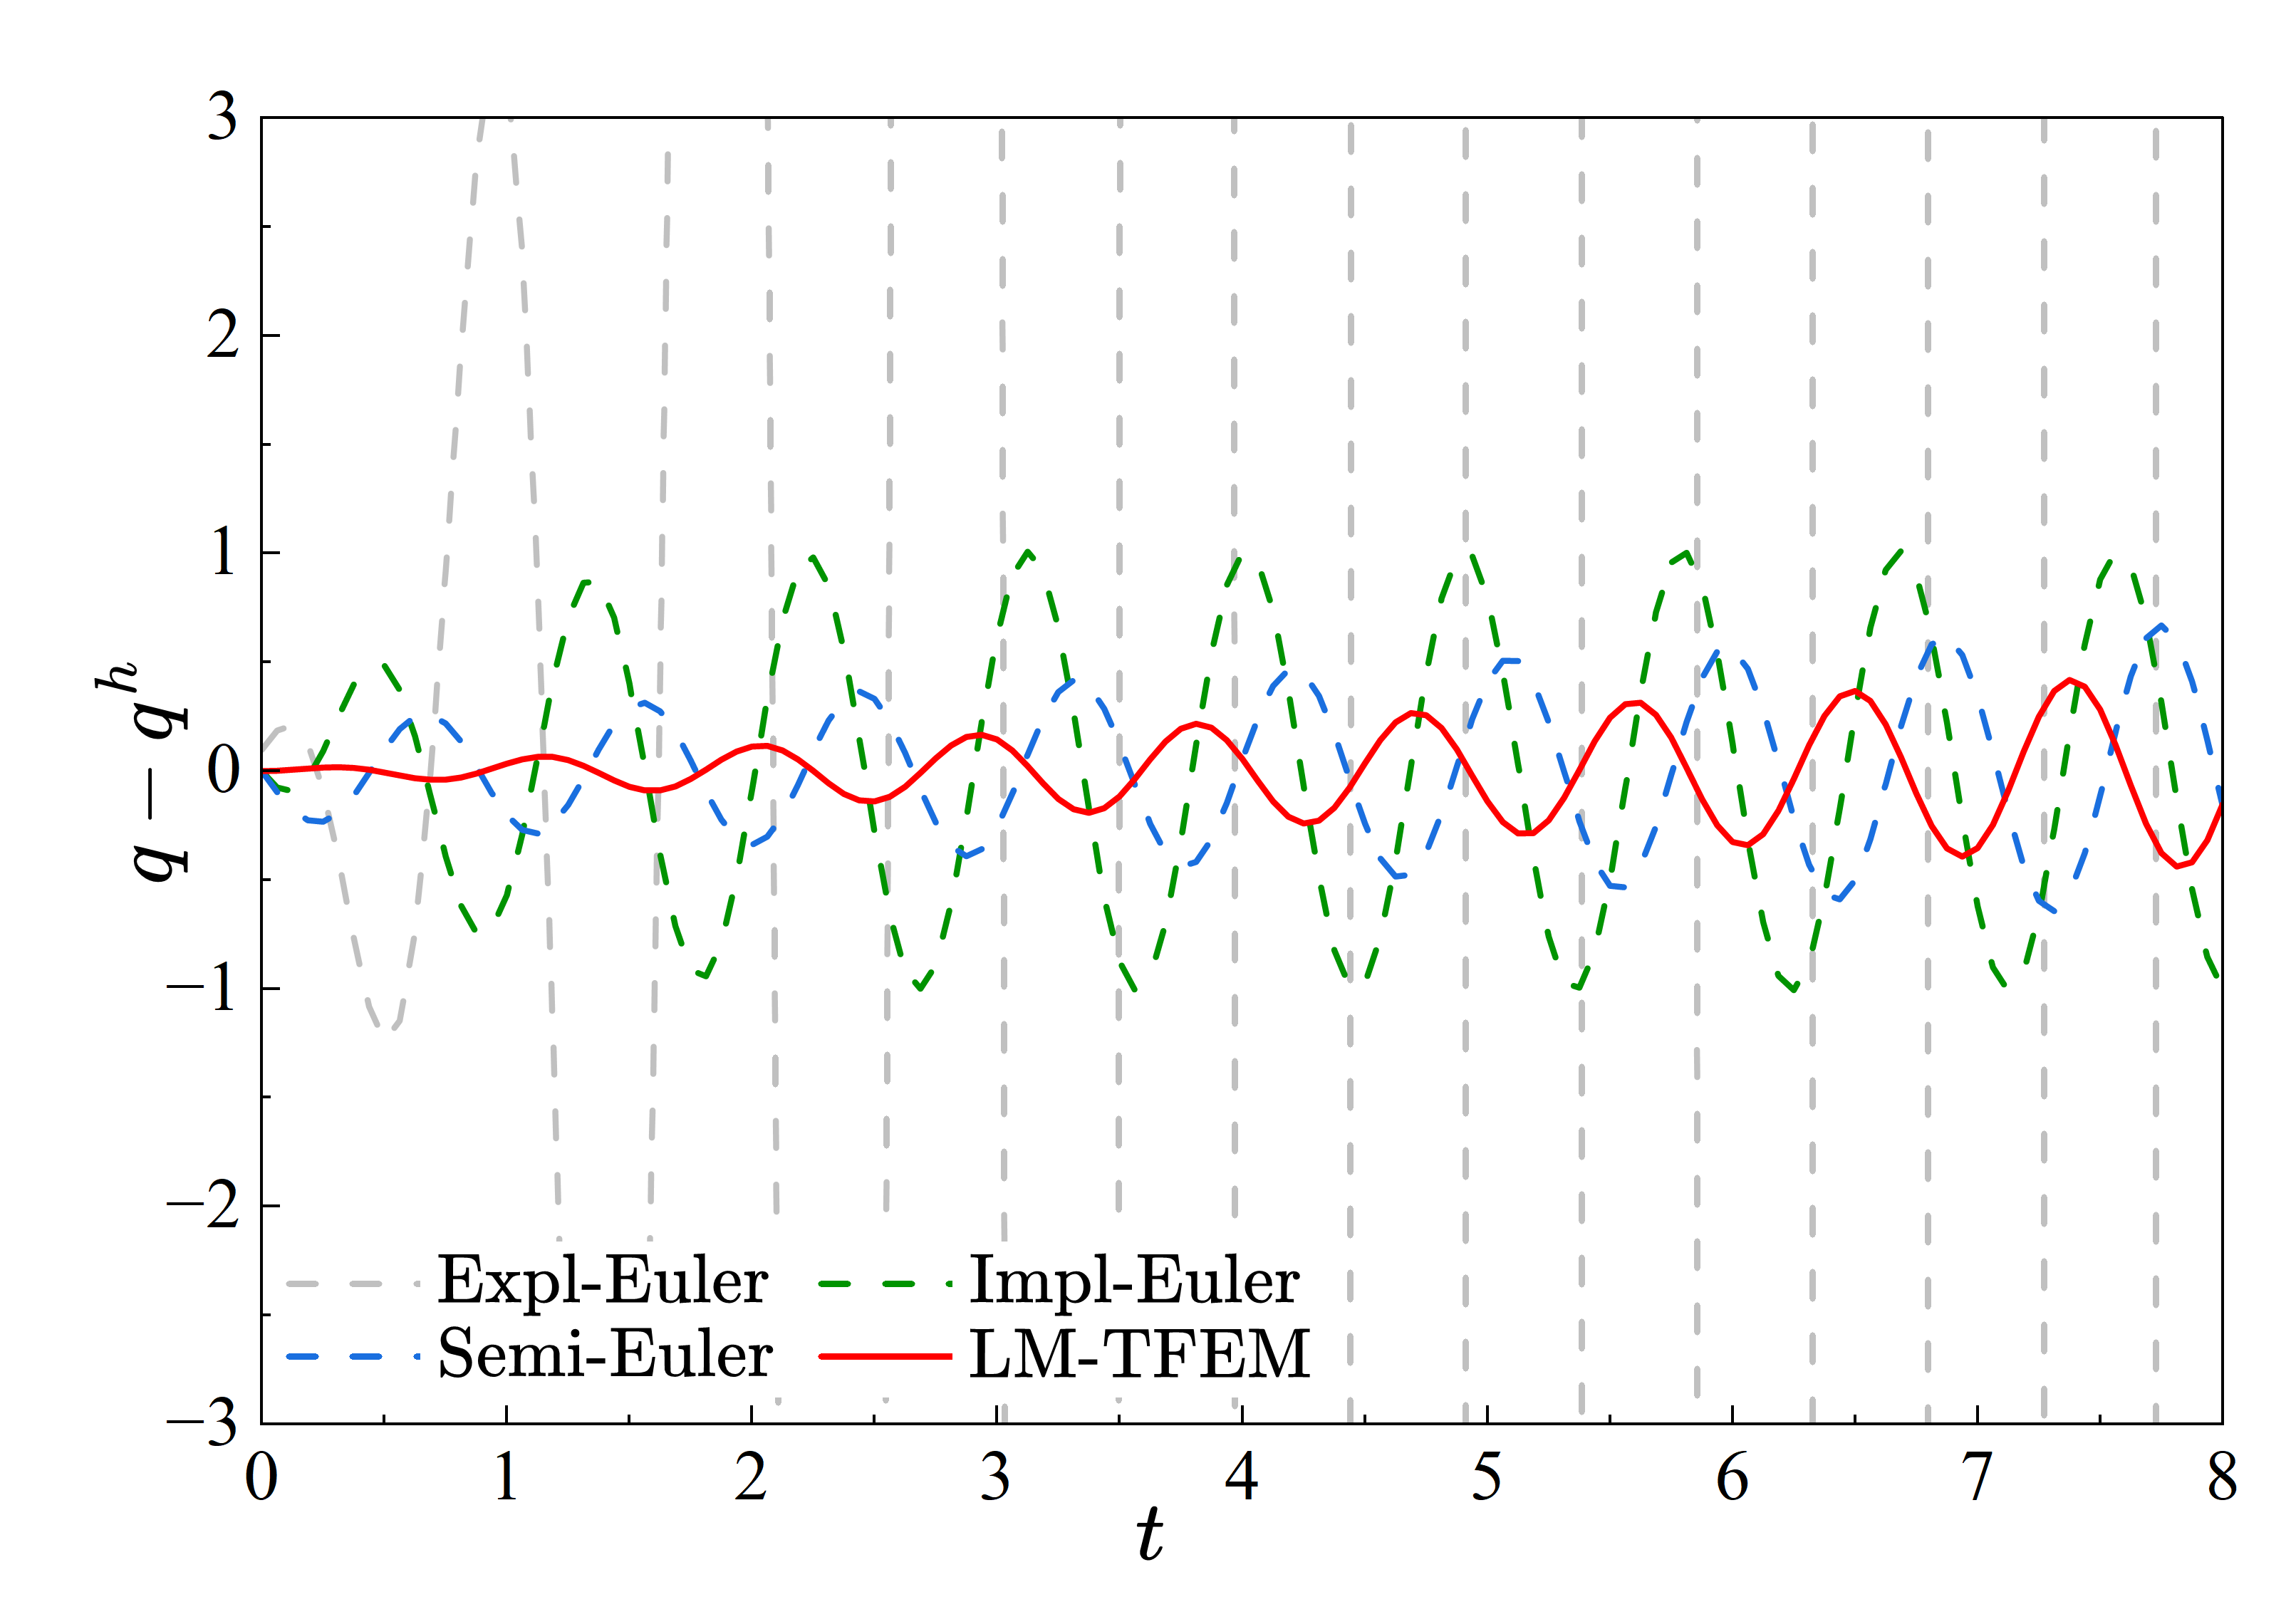
\includegraphics[width=0.45\textwidth]{fig/math/Δt=0.0625位移误差图.png} \\
        \end{tabular}
        \caption{$\Delta t=0.0625$时四种方法计算弹簧小车问题的位移图与误差图}\label{fg:0.0625}
\end{figure}
\begin{figure}[!h]
    \centering
        \begin{tabular}{c@{\hspace{15pt}}c}
            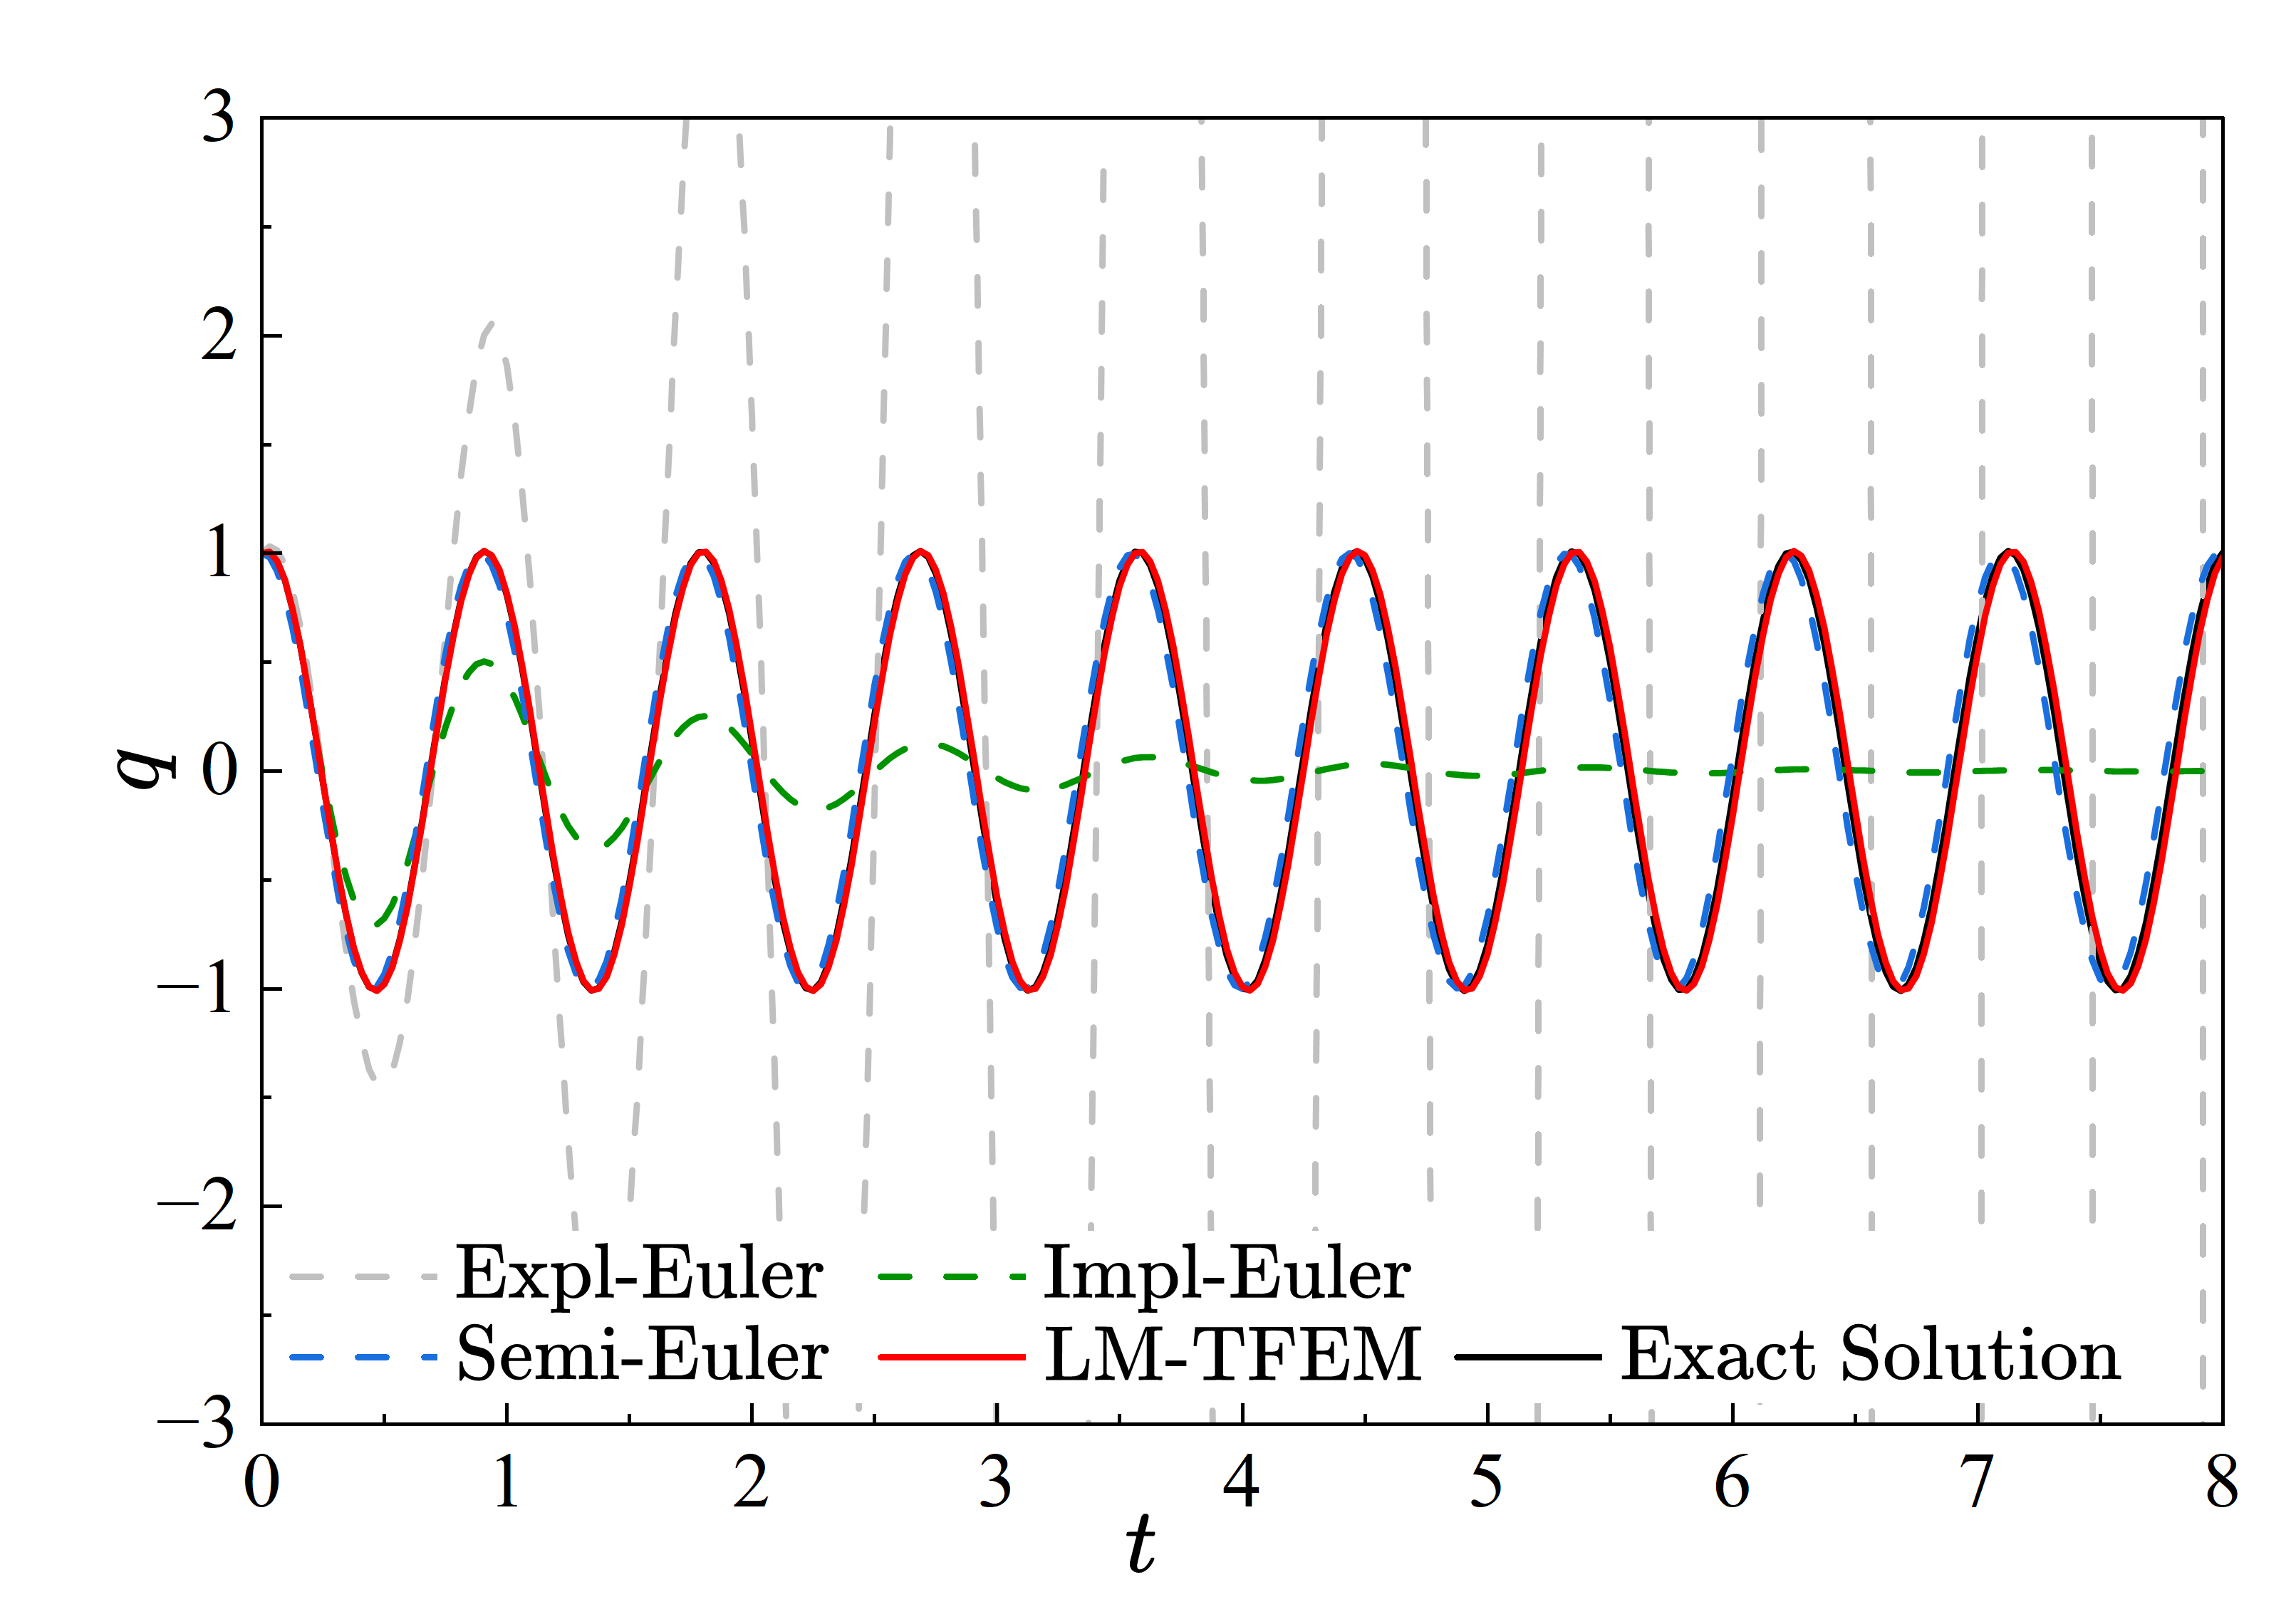
\includegraphics[width=0.45\textwidth]{fig/math/Δt=0.03125位移图.png} &
            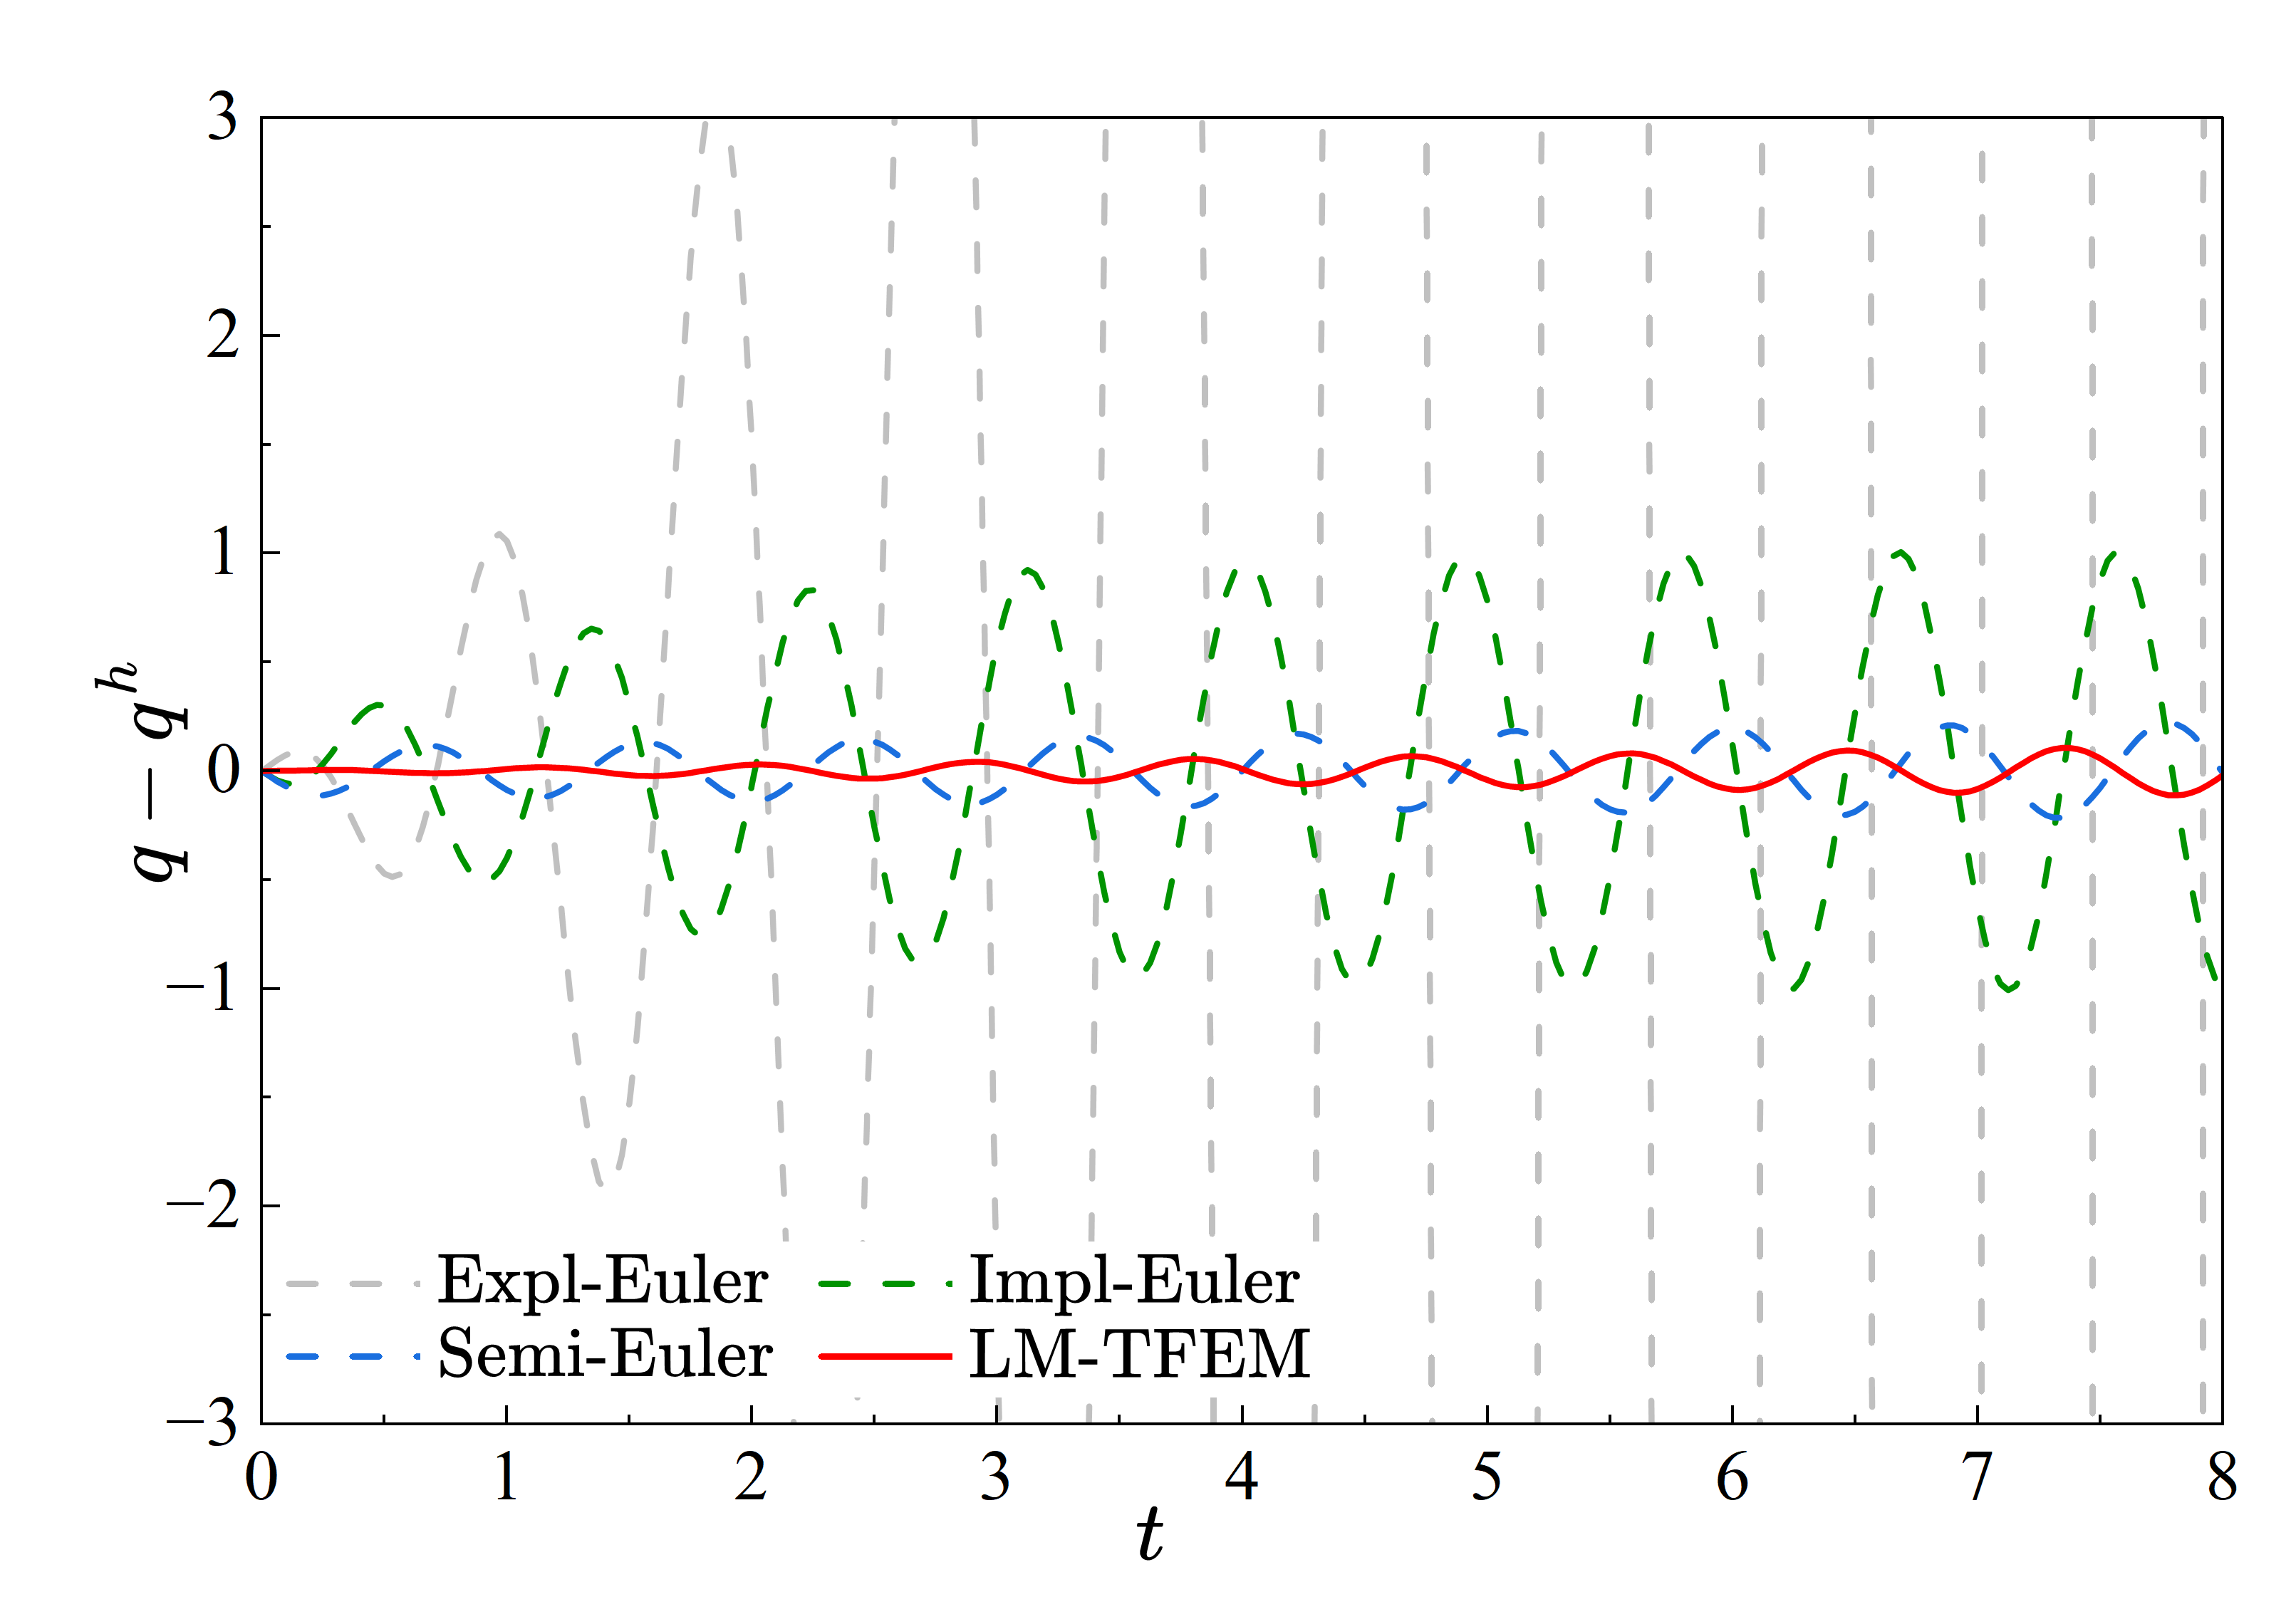
\includegraphics[width=0.45\textwidth]{fig/math/Δt=0.03125位移误差图.png} \\
        \end{tabular}
        \caption{$\Delta t=0.03125$时四种方法计算弹簧小车问题的位移图与误差图}\label{fg:0.03125}
\end{figure}

\begin{figure}[!h]
    \centering
    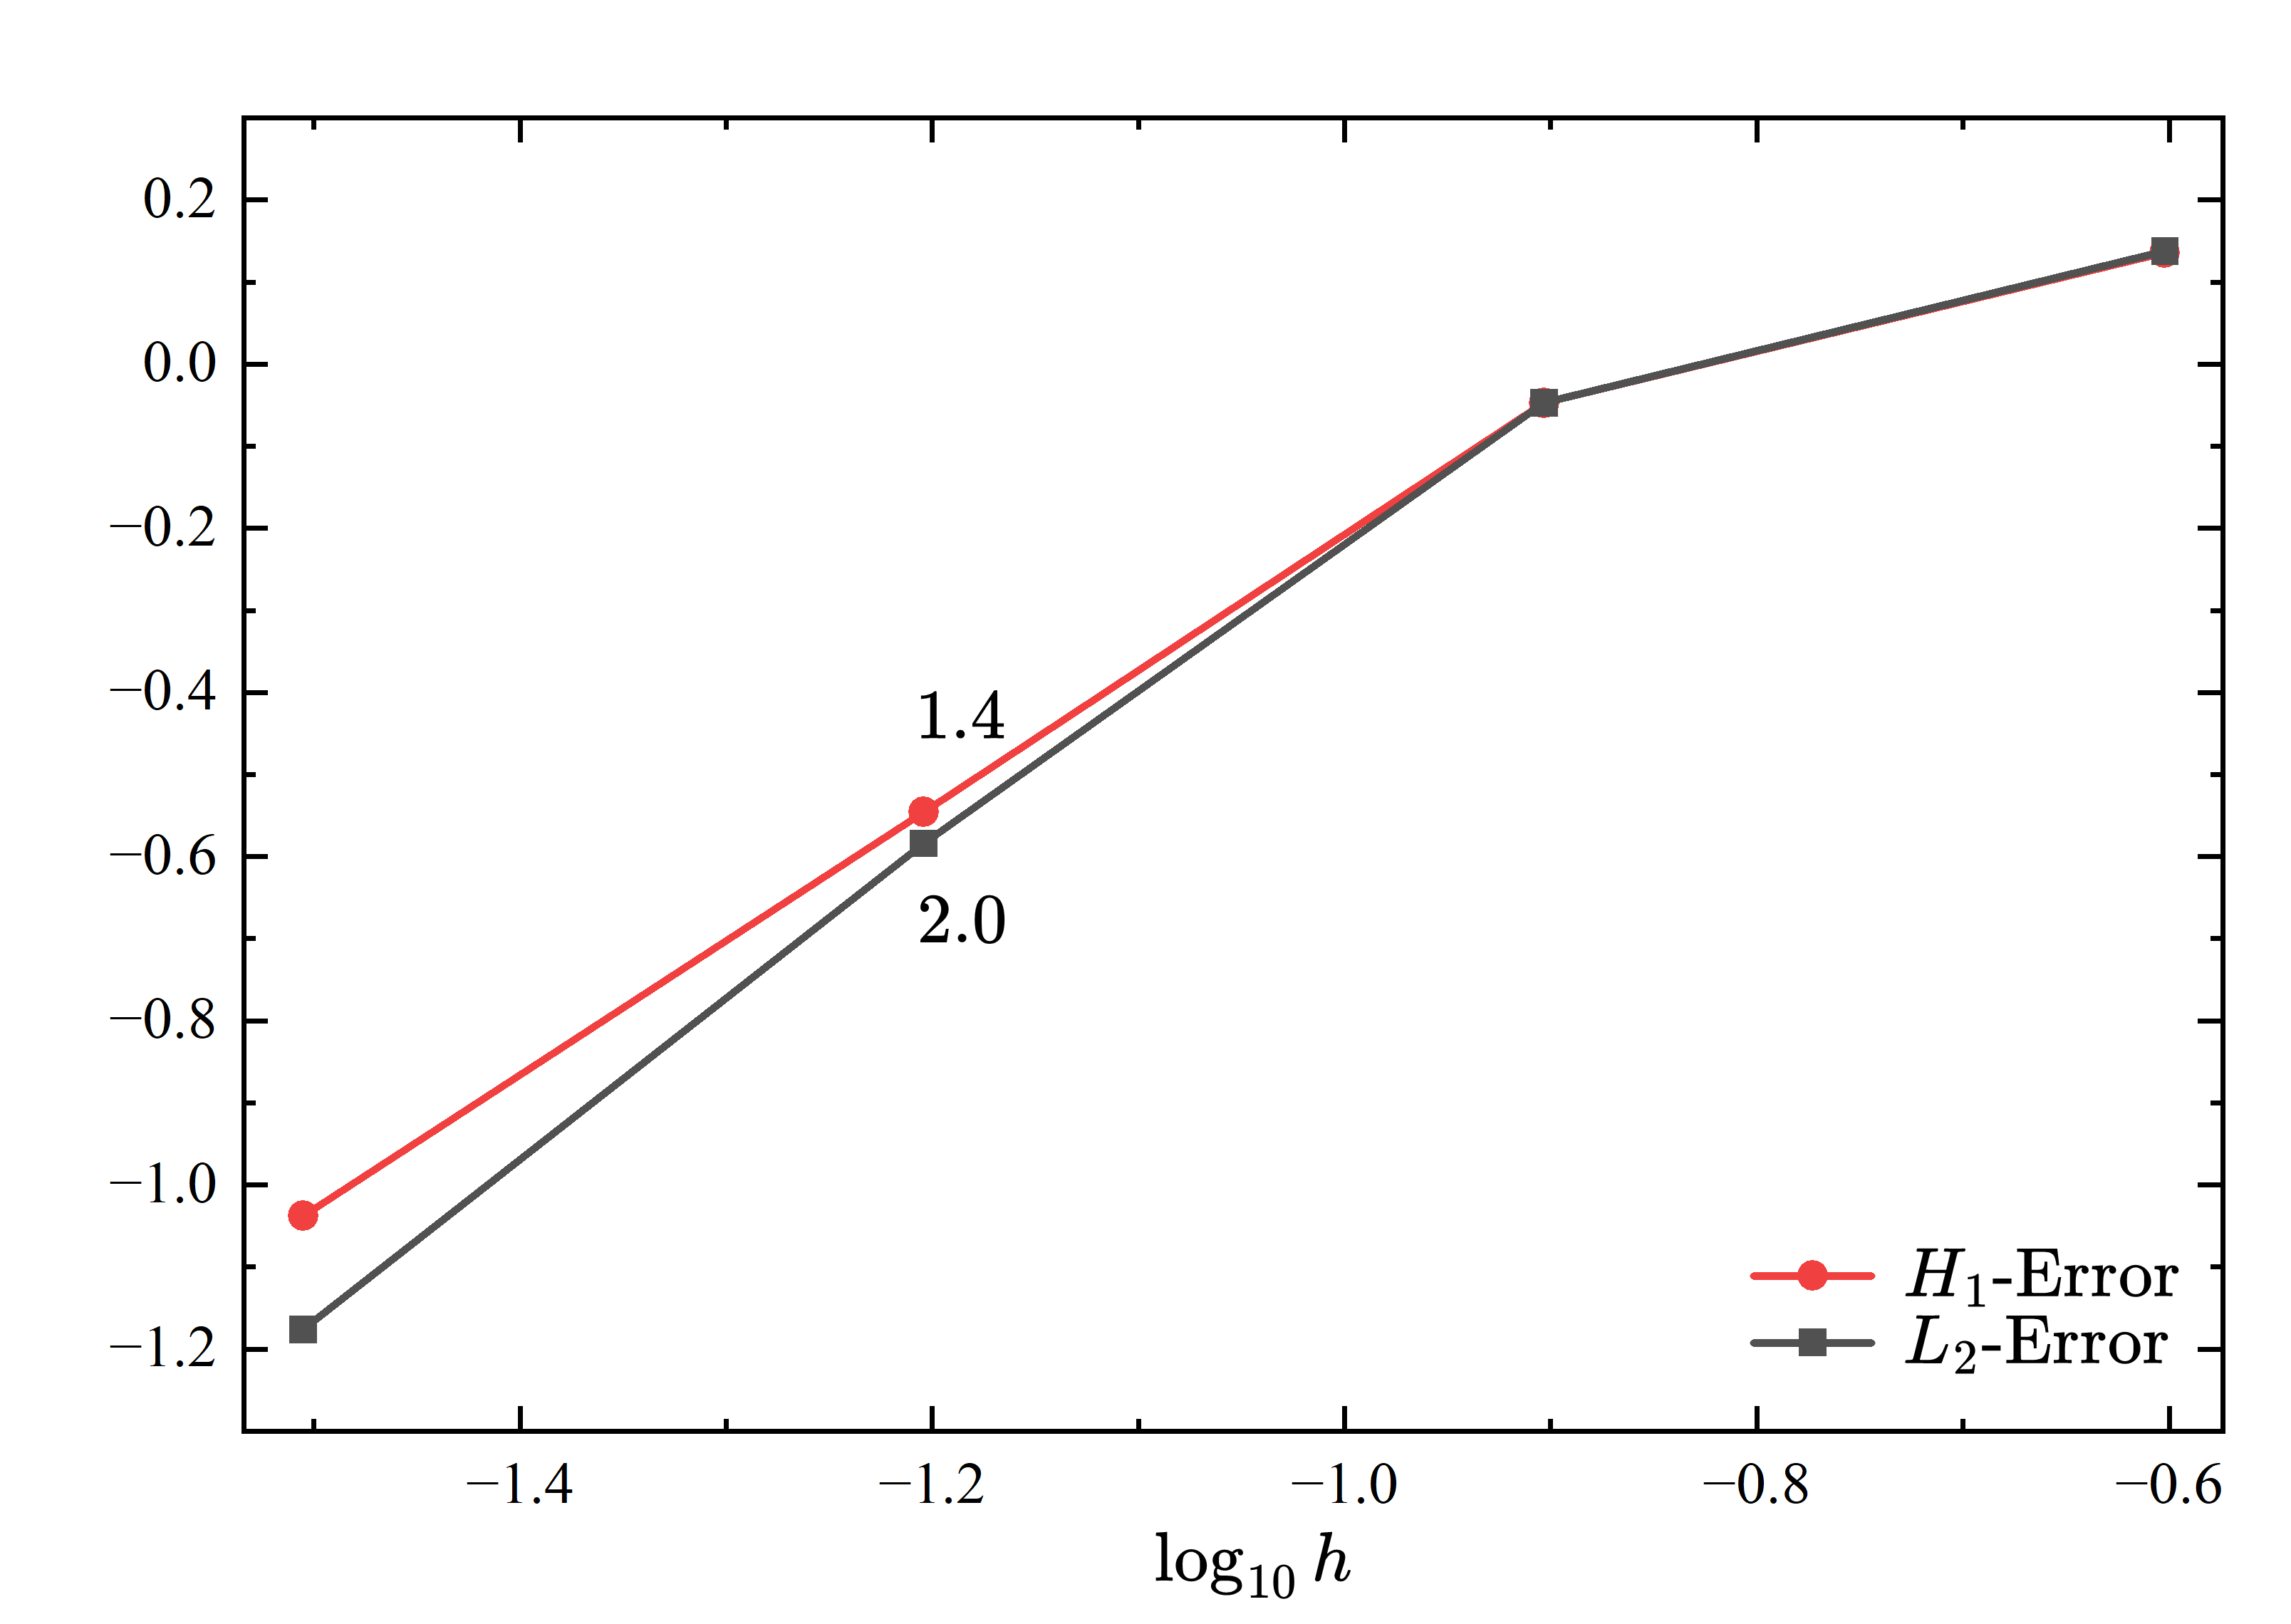
\includegraphics[scale=0.38]{fig/math/波长根号50的L2收敛图.png}
\caption{\centering{弹簧小车问题误差收敛结果}}
\label{fg:tanhuangxiaocheL2}
\end{figure}

同样的，采取一样的节点密度，但采用如图\ref{fg:unbar}所示的非均布网格，
在拉格朗日乘子时空混合离散计算下，也可以得到如图\ref{fg:tanhuangxiaochefeijunbuL2}所示的$2.0$的位移误差收敛率，
达到理论的误差收敛率。

\begin{figure}[!h]
    \centering
        \begin{tabular}{c}
            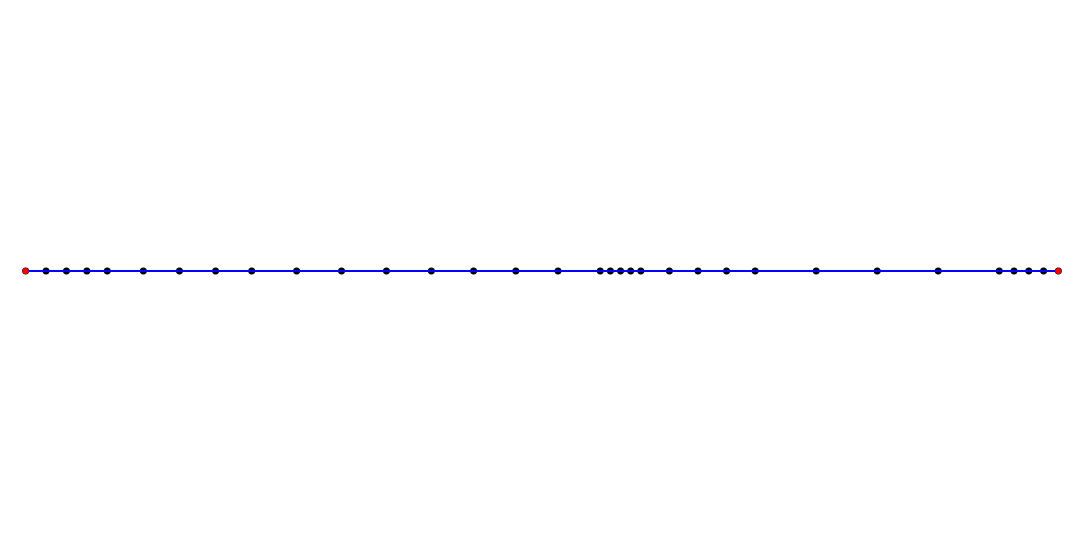
\includegraphics[width=0.8\textwidth]{fig/math/un_n=32.png} \\
            $n=32$ \\
            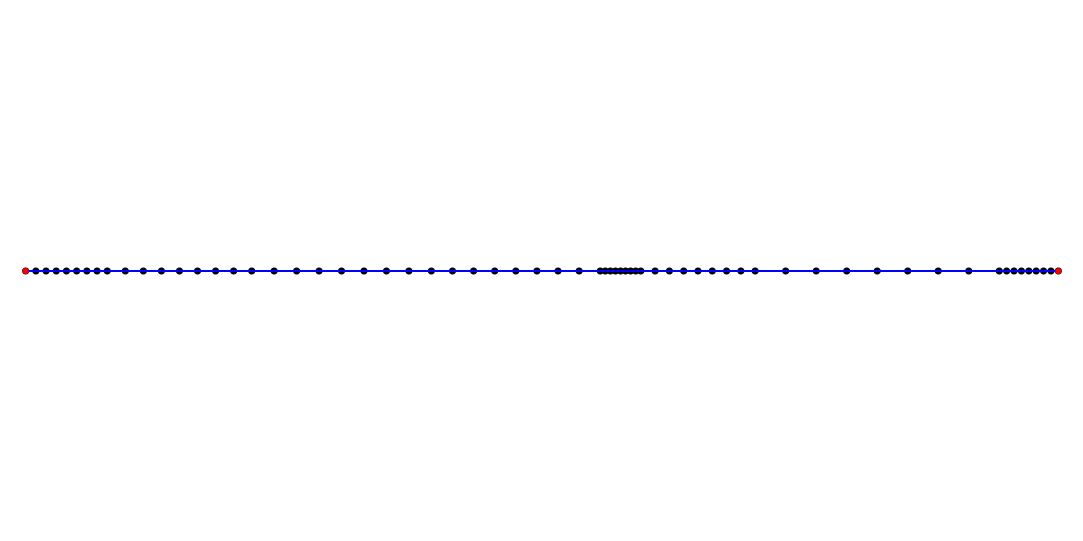
\includegraphics[width=0.8\textwidth]{fig/math/un_n=64.png} \\
            $n=64$ \\
            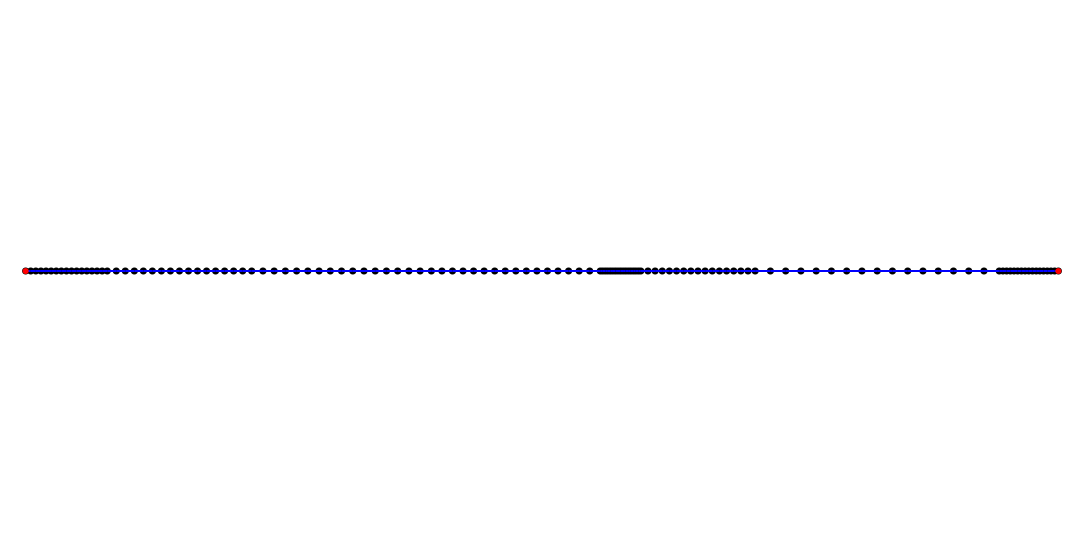
\includegraphics[width=0.8\textwidth]{fig/math/un_n=128.png} \\
            $n=128$ \\
            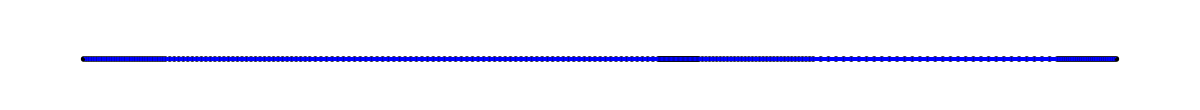
\includegraphics[width=0.8\textwidth]{fig/math/un_n=256.png} \\
            $n=256$
        \end{tabular}
        \caption{弹性小车问题节点非均布布置示意图}\label{fg:unbar}
\end{figure}


\begin{figure}[!h]
    \centering
    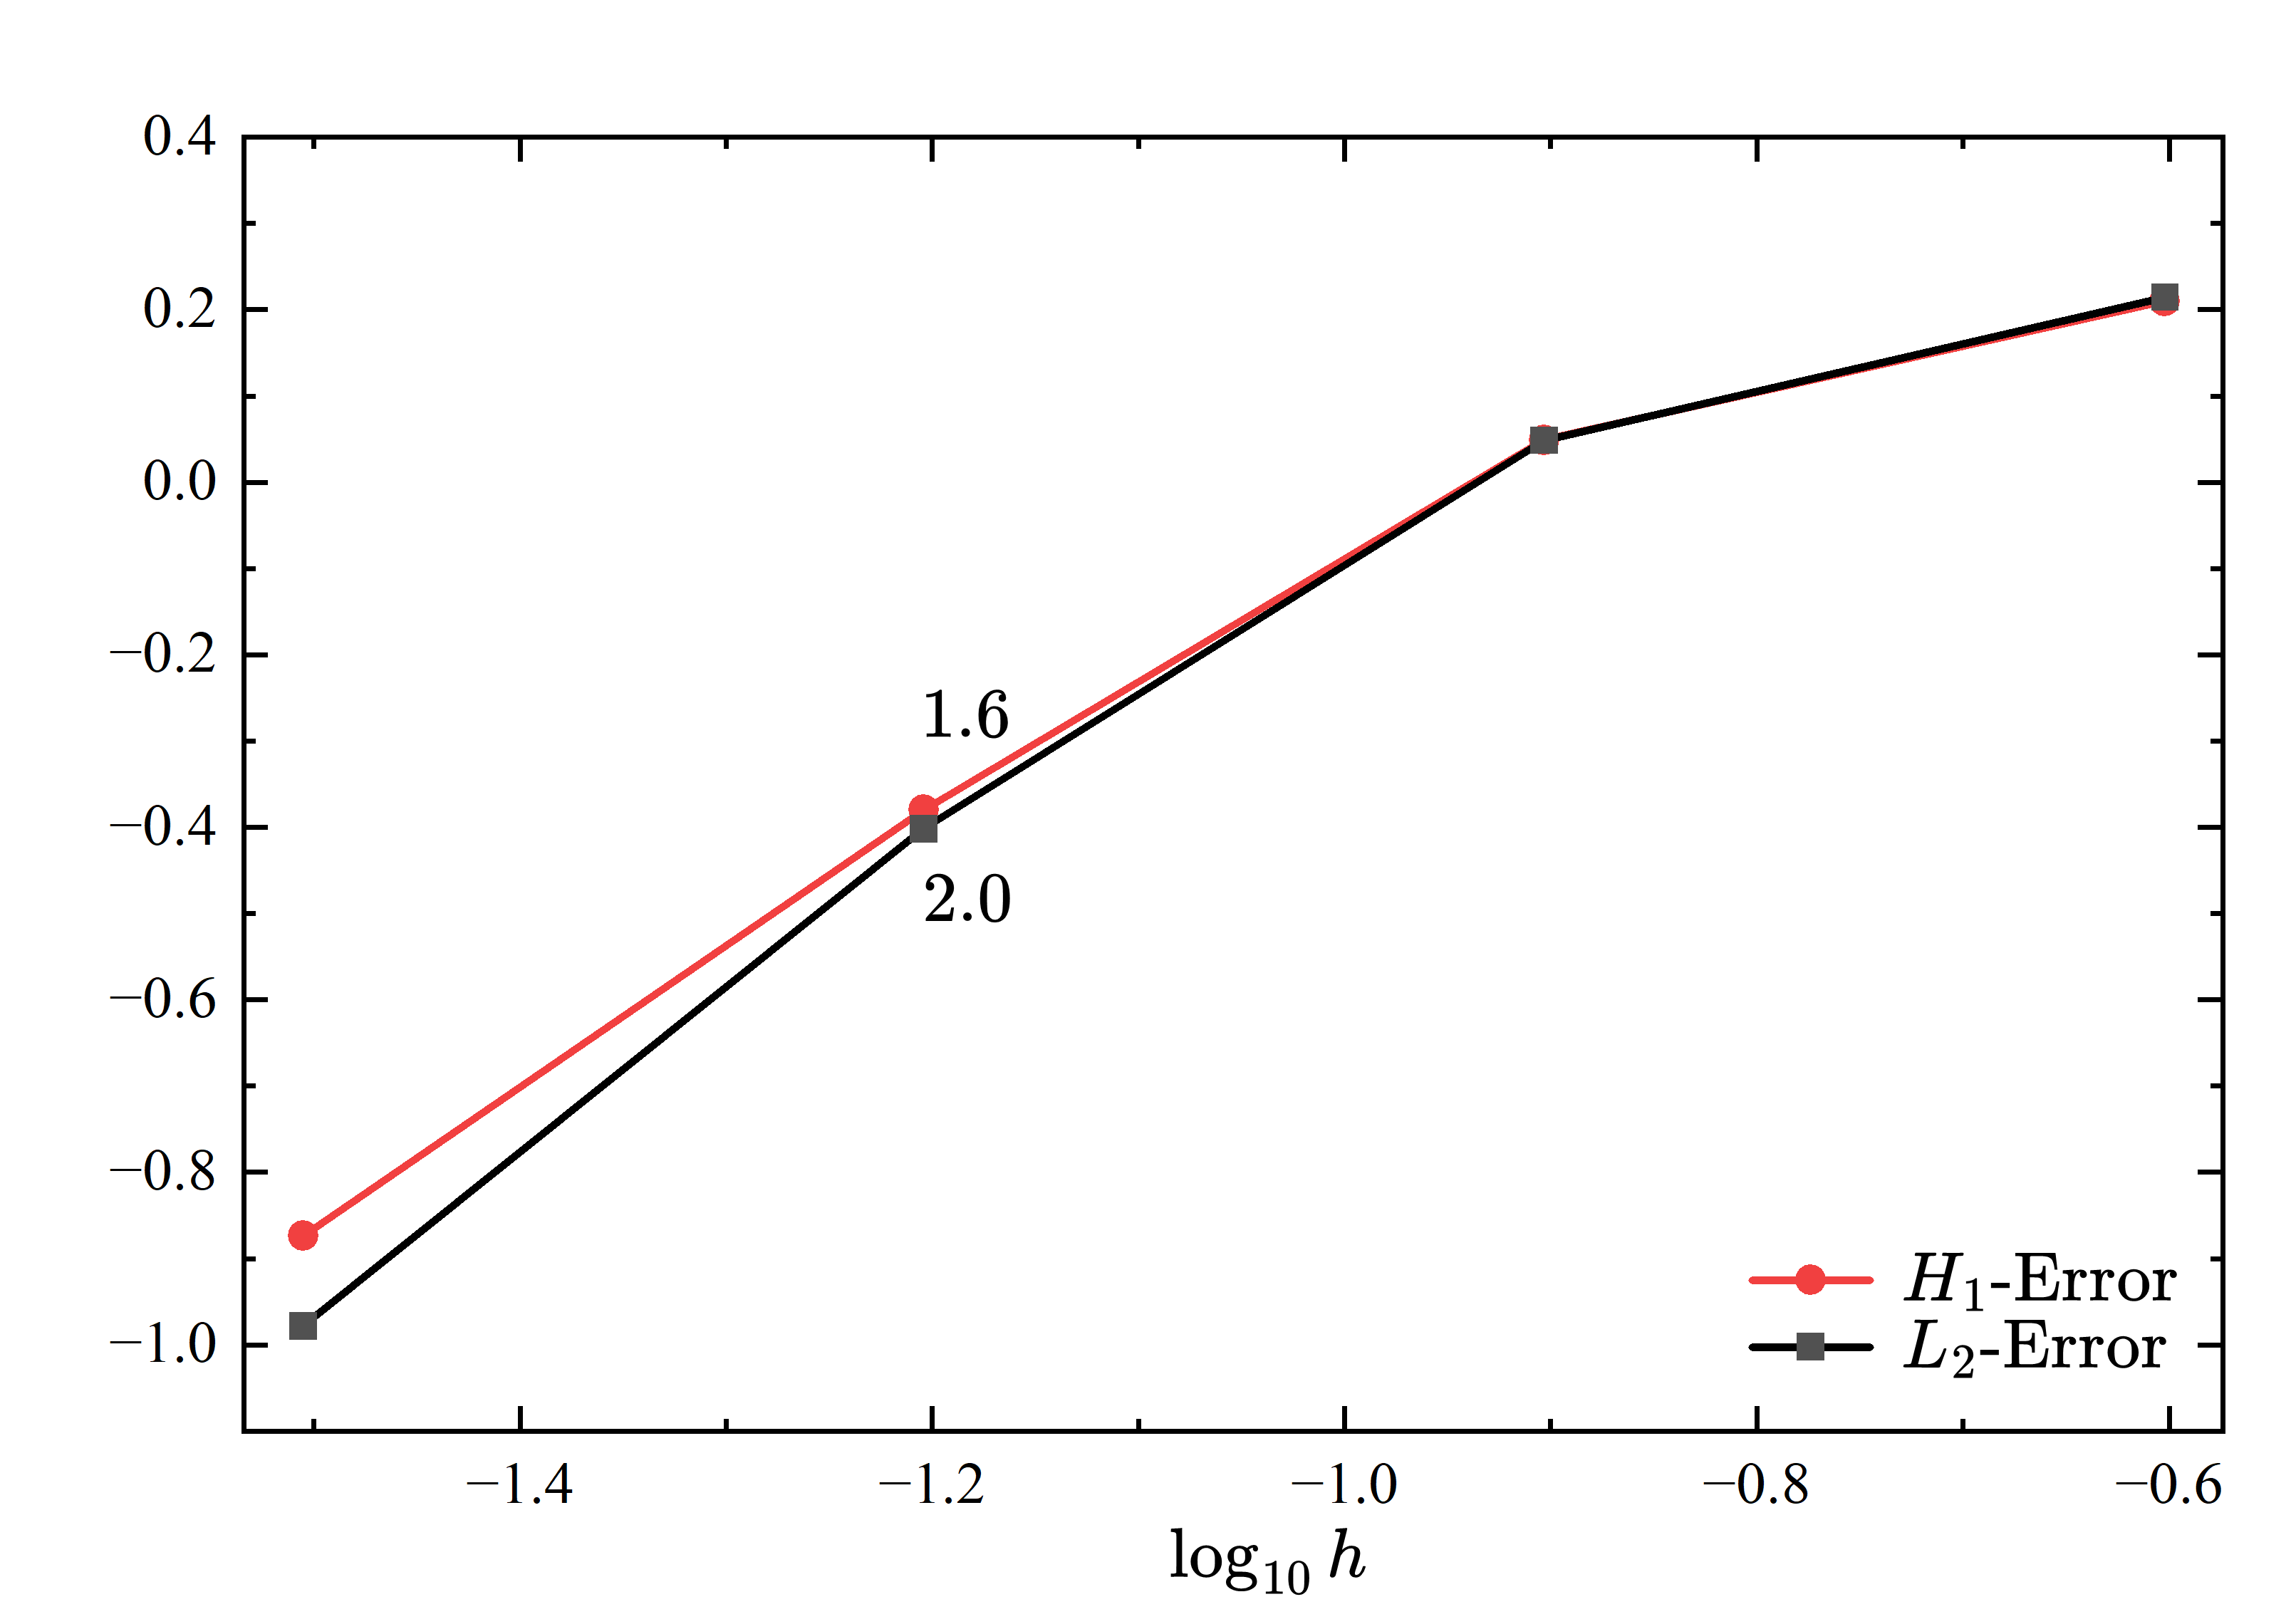
\includegraphics[scale=0.38]{fig/math/波长根号50的非均布L2收敛图.png}
\caption{\centering{弹簧小车问题非均布网格误差收敛结果}}
\label{fg:tanhuangxiaochefeijunbuL2}
\end{figure}






\subsection{受简谐外力作用的无阻尼弹簧小车问题}

同样的考虑一个一维无阻尼弹簧小车问题，我们在此基础上在额外施加一个随着时间改变的简谐振动力$F(t) = F_0 \sin (\Omega t)$，
其中初始力$F_0=5.0$，驱动频率$\Omega = 25.0$。
如图\ref{fg:jianxiexiaoche}所示，小车的质量$m=1.0$，初始位移$q_0=0$和初始速度$\dot q_0$的作用下运动。
小车的左端仍然施加一个刚度系数为$k=50.0$的弹簧约束，右端不施加任何约束。
取总时间$T=8$，来计算时间步长分别为$0.25,0.125,0.0625,0.03125$情况下的小车运动状态。

\begin{figure}[!h]
    \centering
    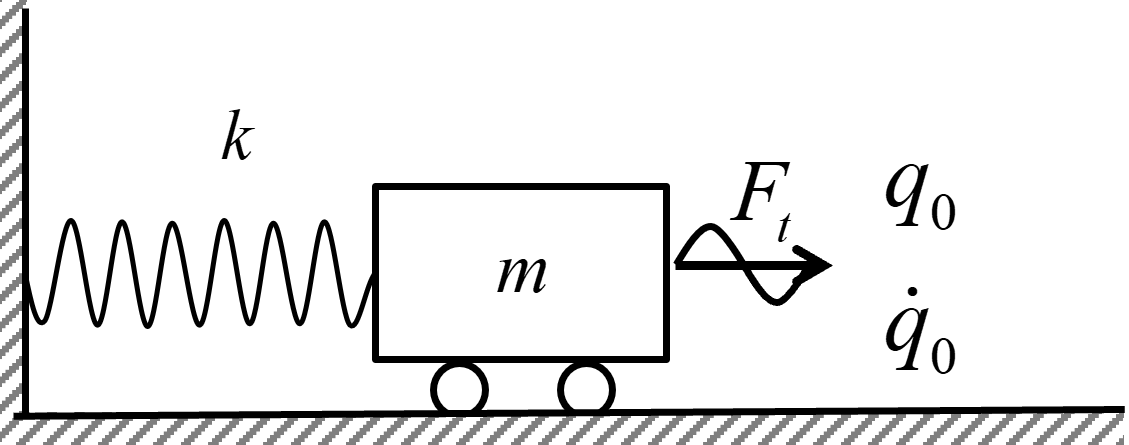
\includegraphics[scale=1.0]{fig/math/简谐弹簧小车模型.png}
\caption{\centering{受简谐作用的无阻尼弹簧小车算例模型}}
\label{fg:jianxiexiaoche}
\end{figure}

根据弹性力学控制方程：
\begin{equation}\label{con found}
m \ddot q + k q = F_0 \sin (\Omega t)
\end{equation}
在给定的初始条件下，其精确解由齐次解和特解组成：
\begin{equation}\label{Exa solu}
\begin{split}
q(t) &= A \cos (\omega t) + B \sin(\omega t) + \frac{F_0}{k-m\Omega^2} sin(\Omega t)
\end{split}
\end{equation}
其中$A = q_0$，$B = \frac{(\dot q_0 - U_0 * \Omega)}{\omega}$，
$U_0 = \frac{F_0}{(k - m * \Omega^2)}$。

通过解析解方程我们可以采用Newmark-$\beta$法对它进行动力分析，
根据式\ref{newmark-explicit}-\ref{newmark-semi-implicit}
所提到的在计算时，根据$\gamma$和$\beta$的取值不同，区分的三种迭代法进行测试。
最后根据Newmark-$\beta$法得到计算结果，
和我们所提出的基于拉格朗日变分方案的哈密顿法的计算结果作对比来测试方法的准确性。

弹簧小车的求解域依然通过图\ref{fg:bar}所示采用均布的四种疏密不同的节点进行计算，
其中节点个数$n=32-256$分别对应$\Delta t=0.25-0.03125$的时间步长。

根据图\ref{fg:jx0.25}-\ref{fg:jx0.03125}的位移以及位移误差计算结果可以看出，
本文所提出的基于拉格朗日乘子型的变分方案计算该算例可以得到目前最精确的数值，
计算误差最小的同时还能保证计算的稳定性。
当我们波速取$\omega=\sqrt{50}$时，节点密度采取$32,64,128,256$四种形式，
来测试基于拉格朗日变分方案的哈密顿完全弱形式法的误差收敛率时，
可以得到如图\ref{fg:jxtanhuangxiaocheL2}所示的$2.0$的位移误差收敛率，
达到理论的误差收敛率，证明该方案是能够准确收敛的。

\begin{figure}[!h]
    \centering
        \begin{tabular}{c@{\hspace{15pt}}c}
            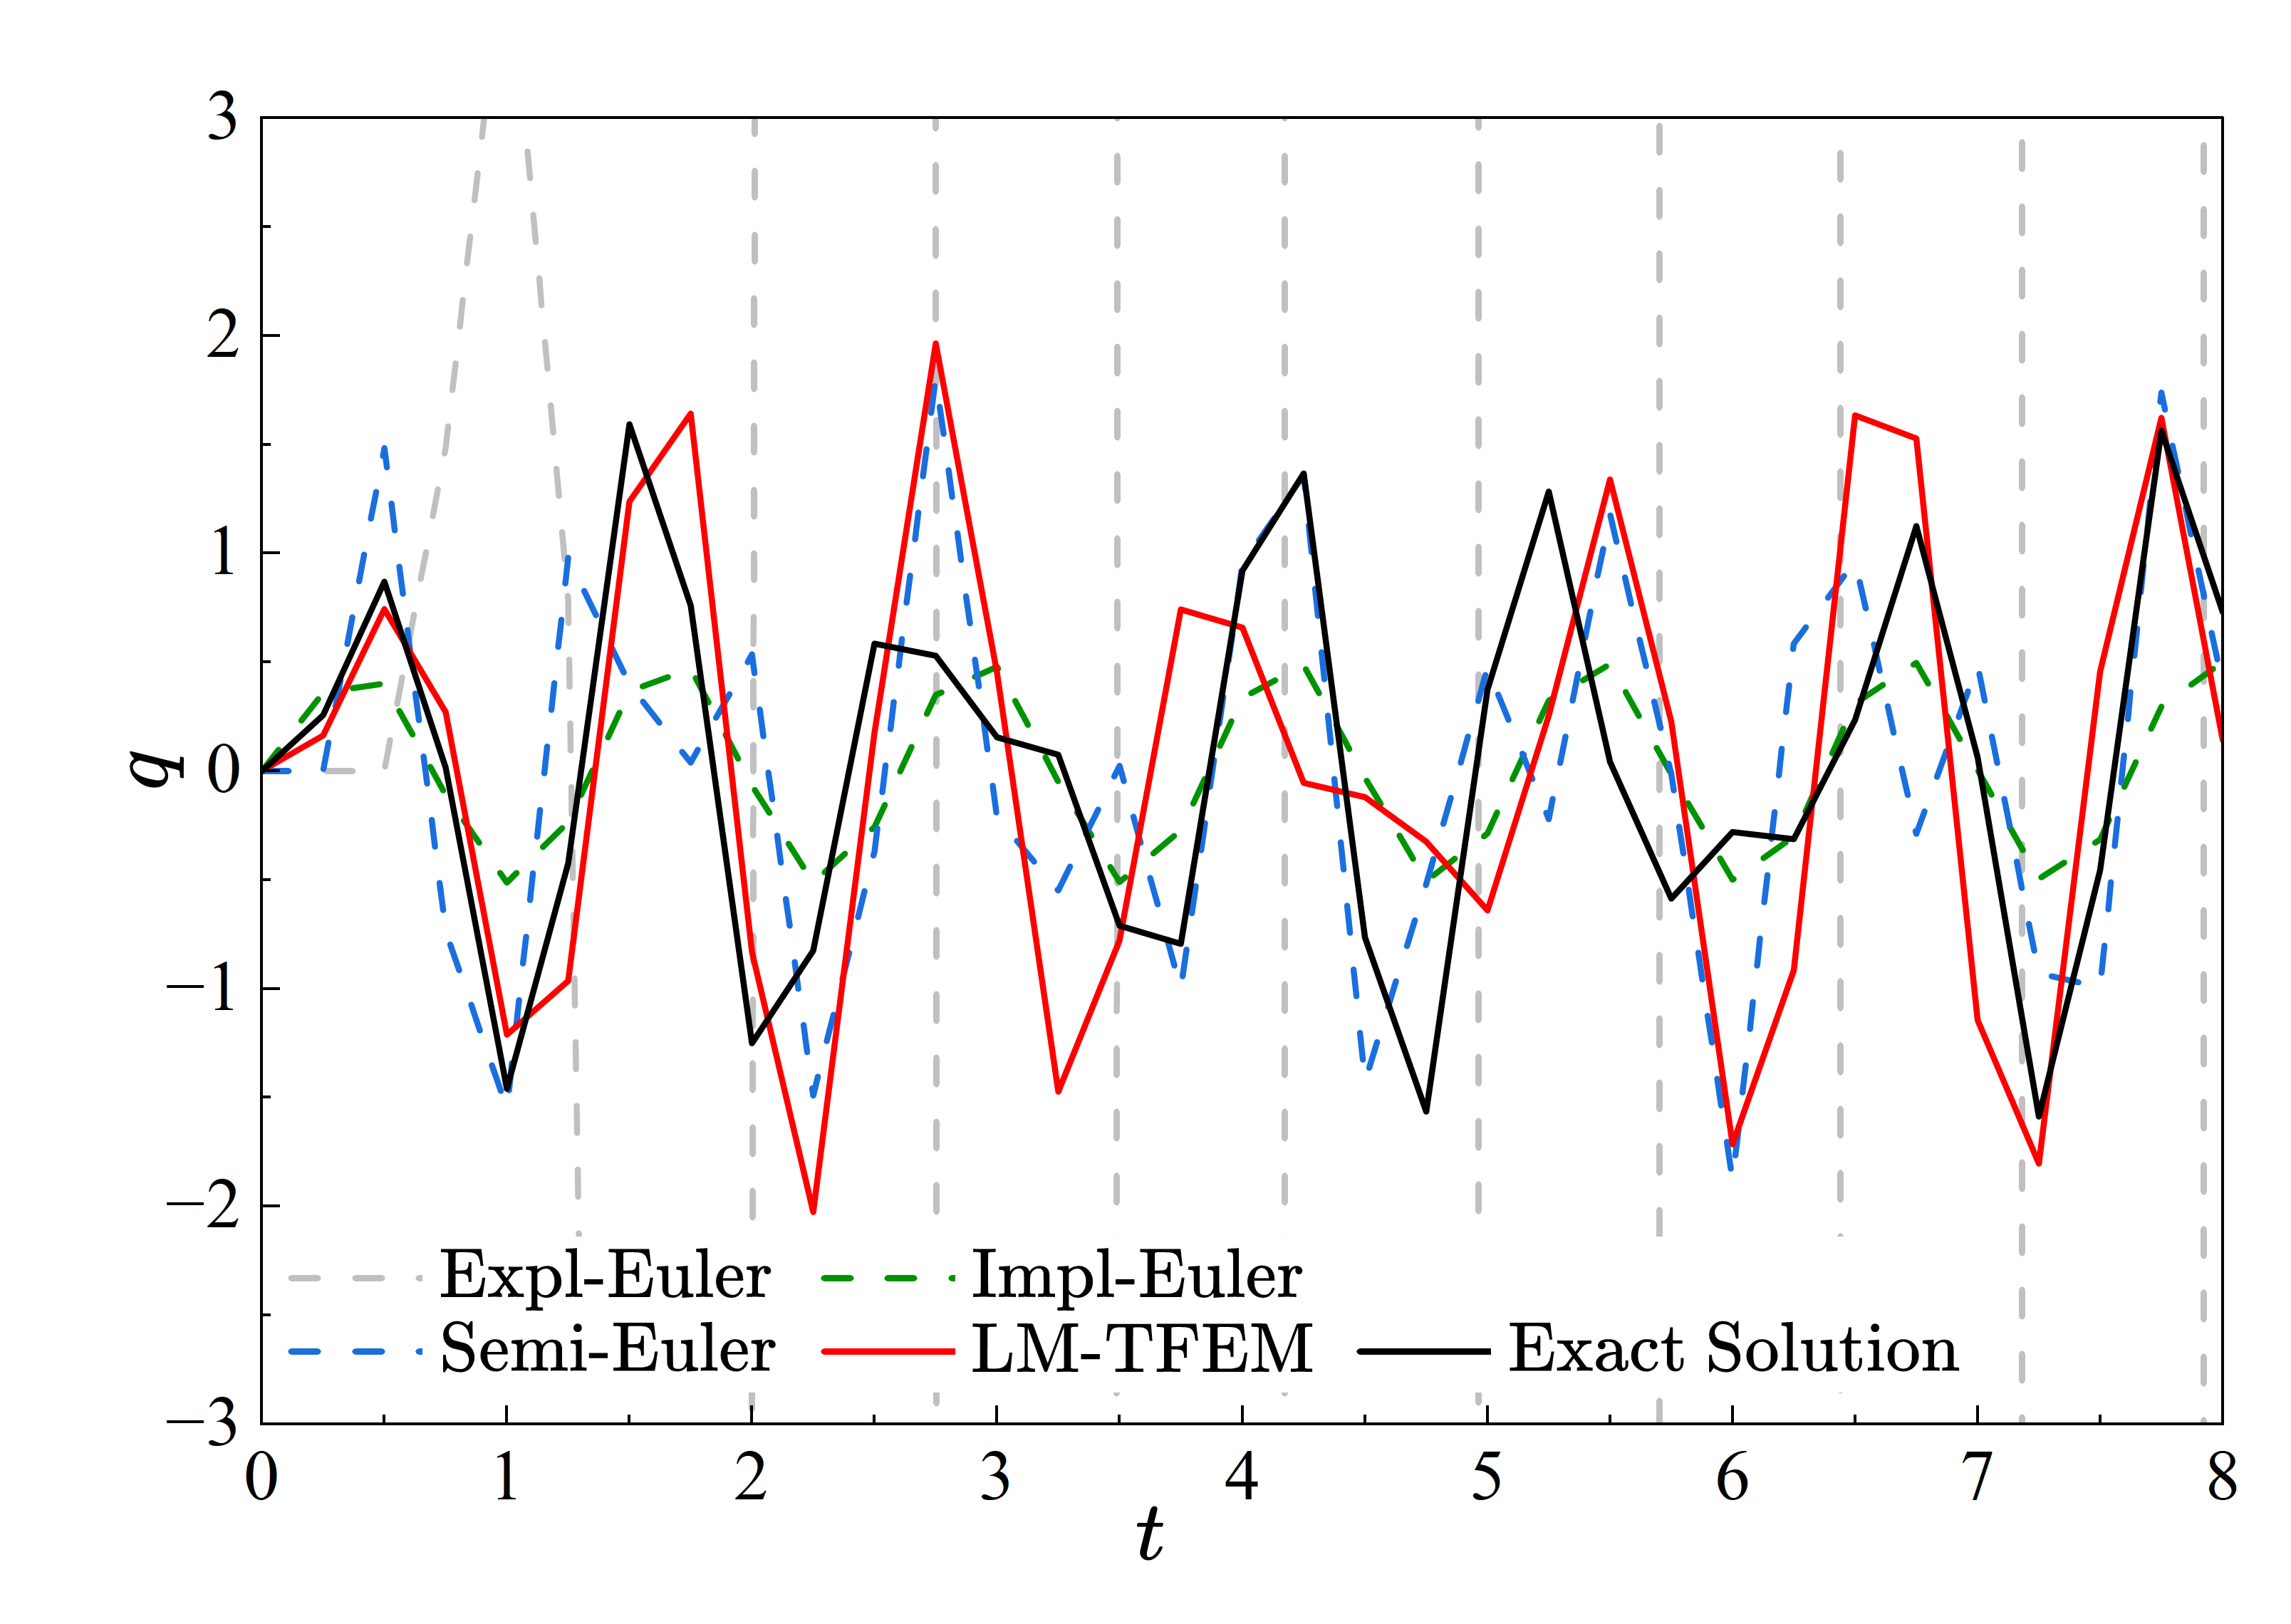
\includegraphics[width=0.45\textwidth]{fig/math/Δt=0.25简谐位移图.png} &
            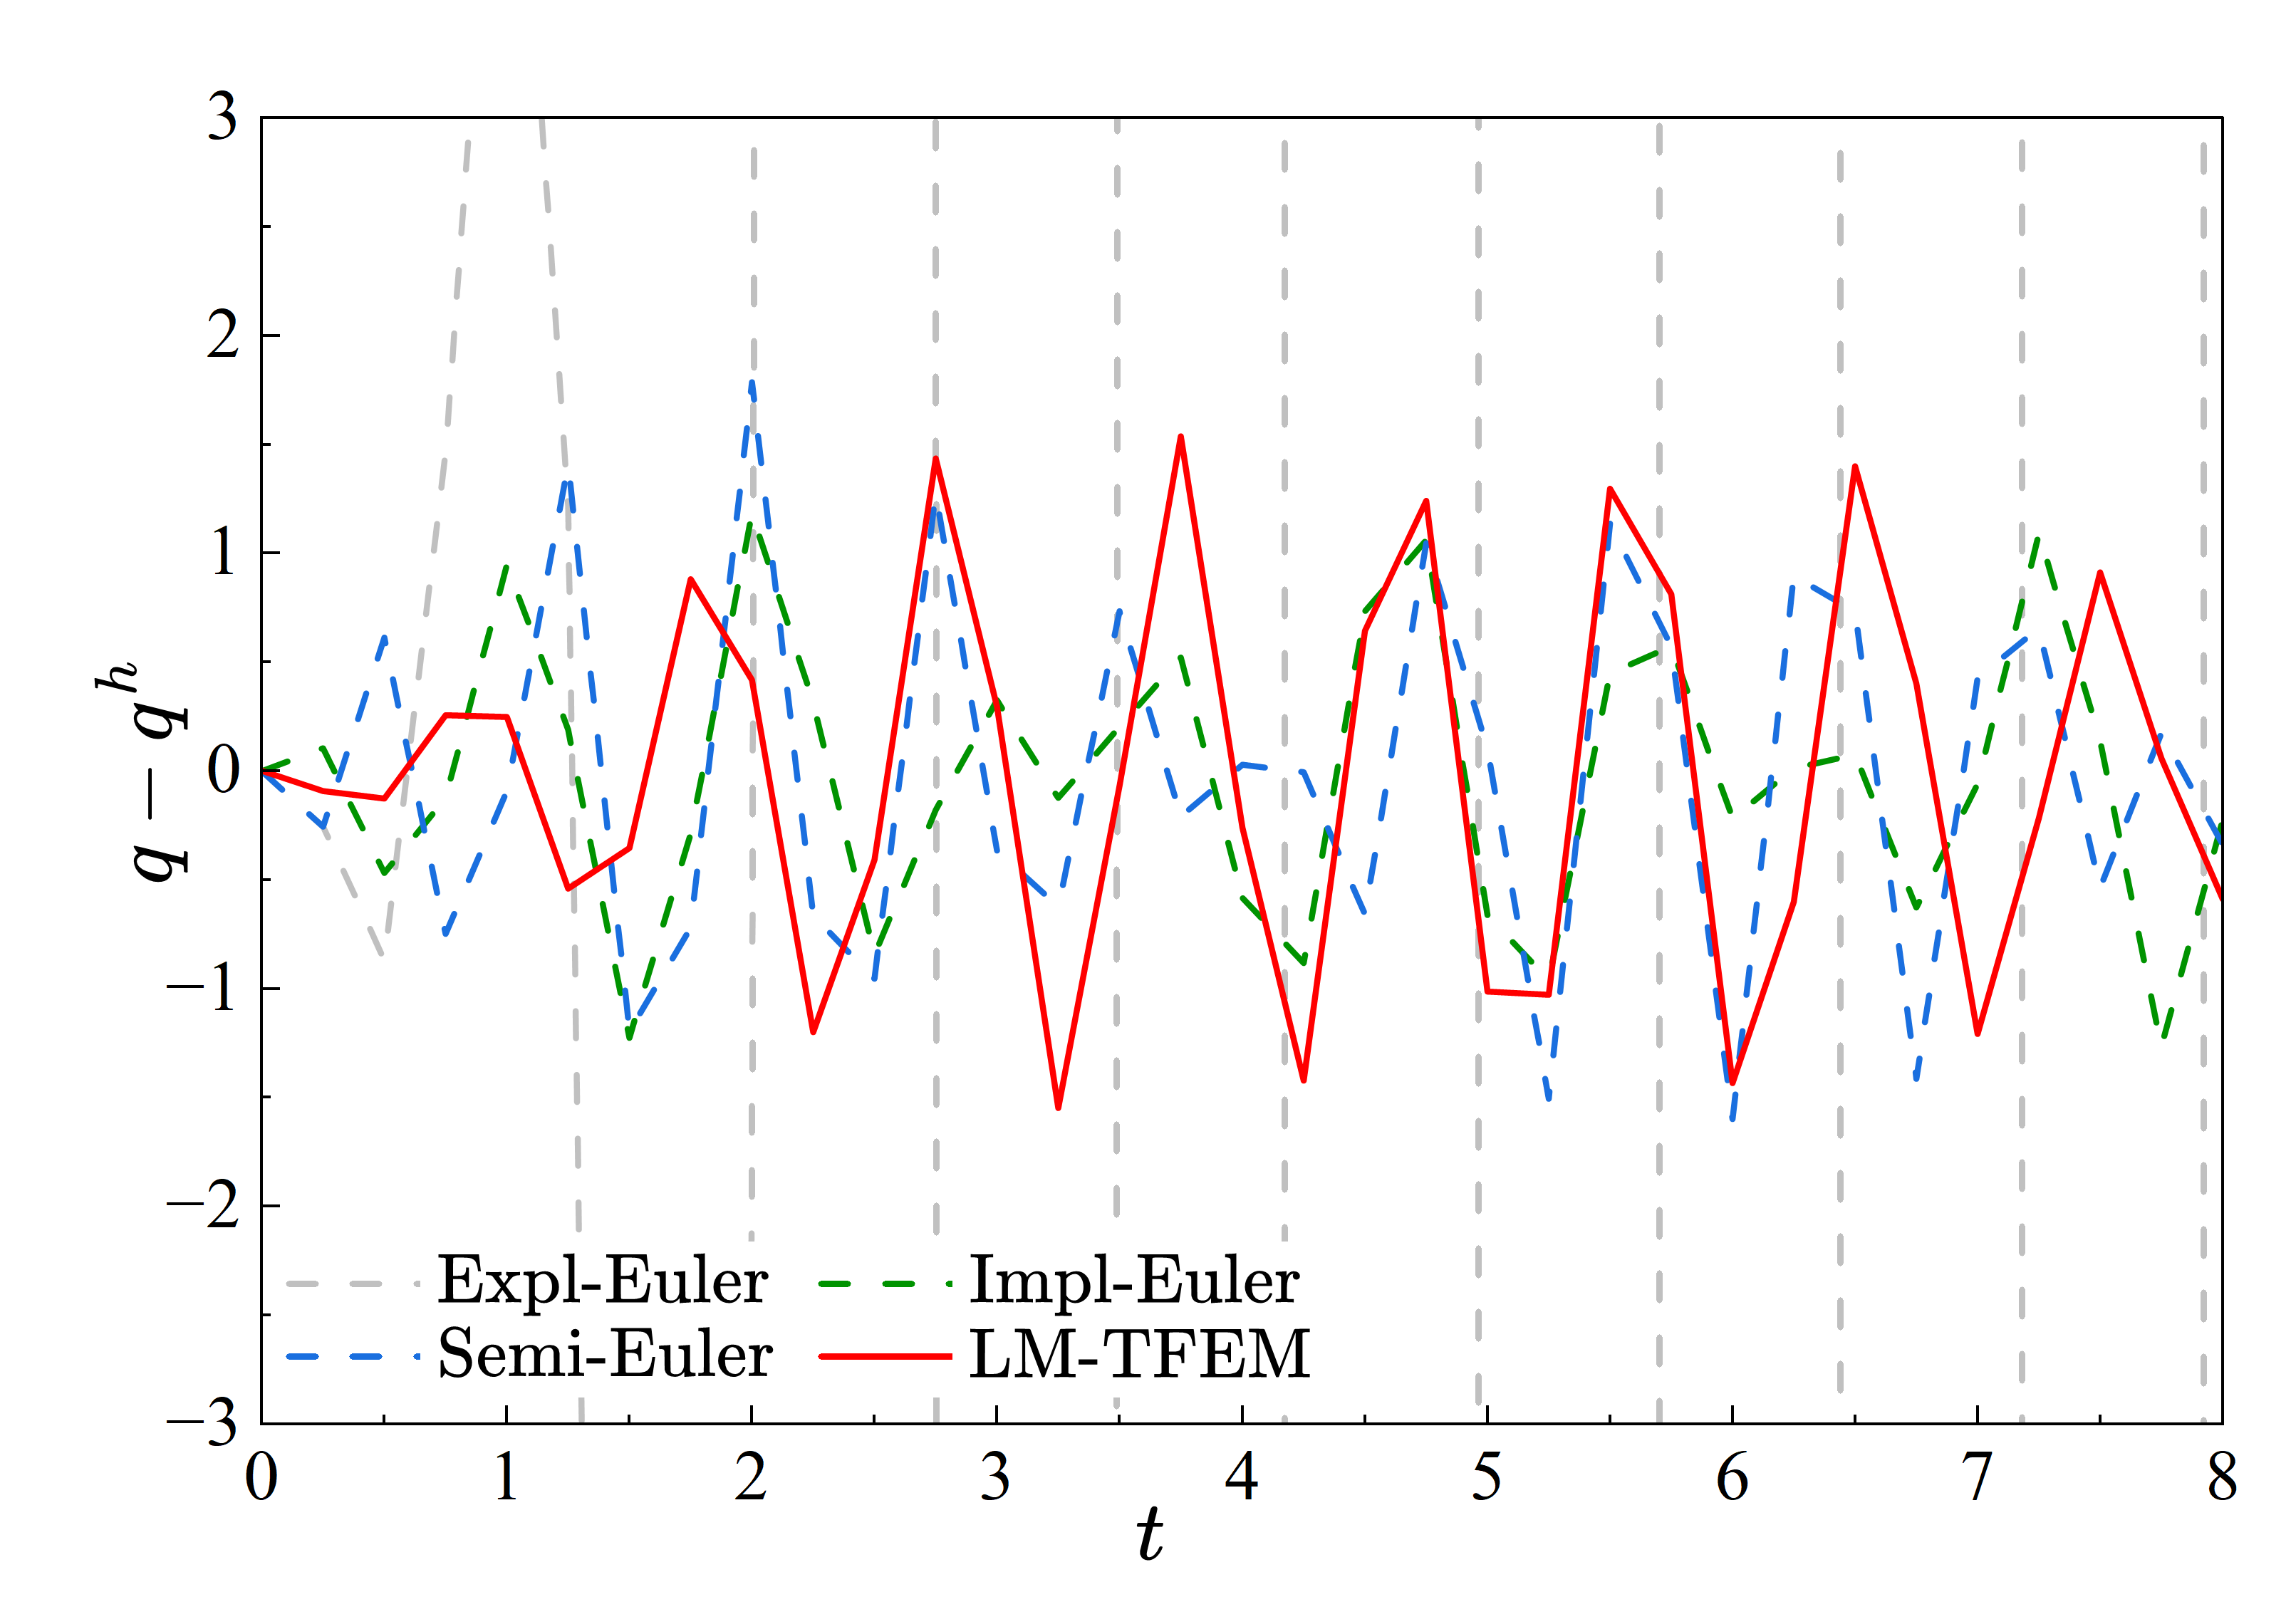
\includegraphics[width=0.45\textwidth]{fig/math/Δt=0.25简谐位移误差图.png} \\
        \end{tabular}
        \caption{$\Delta t=0.25$时四种方法计算简谐外力作用下弹簧小车问题的位移图与误差图}\label{fg:jx0.25}
\end{figure}
\begin{figure}[!h]
    \centering
        \begin{tabular}{c@{\hspace{15pt}}c}
            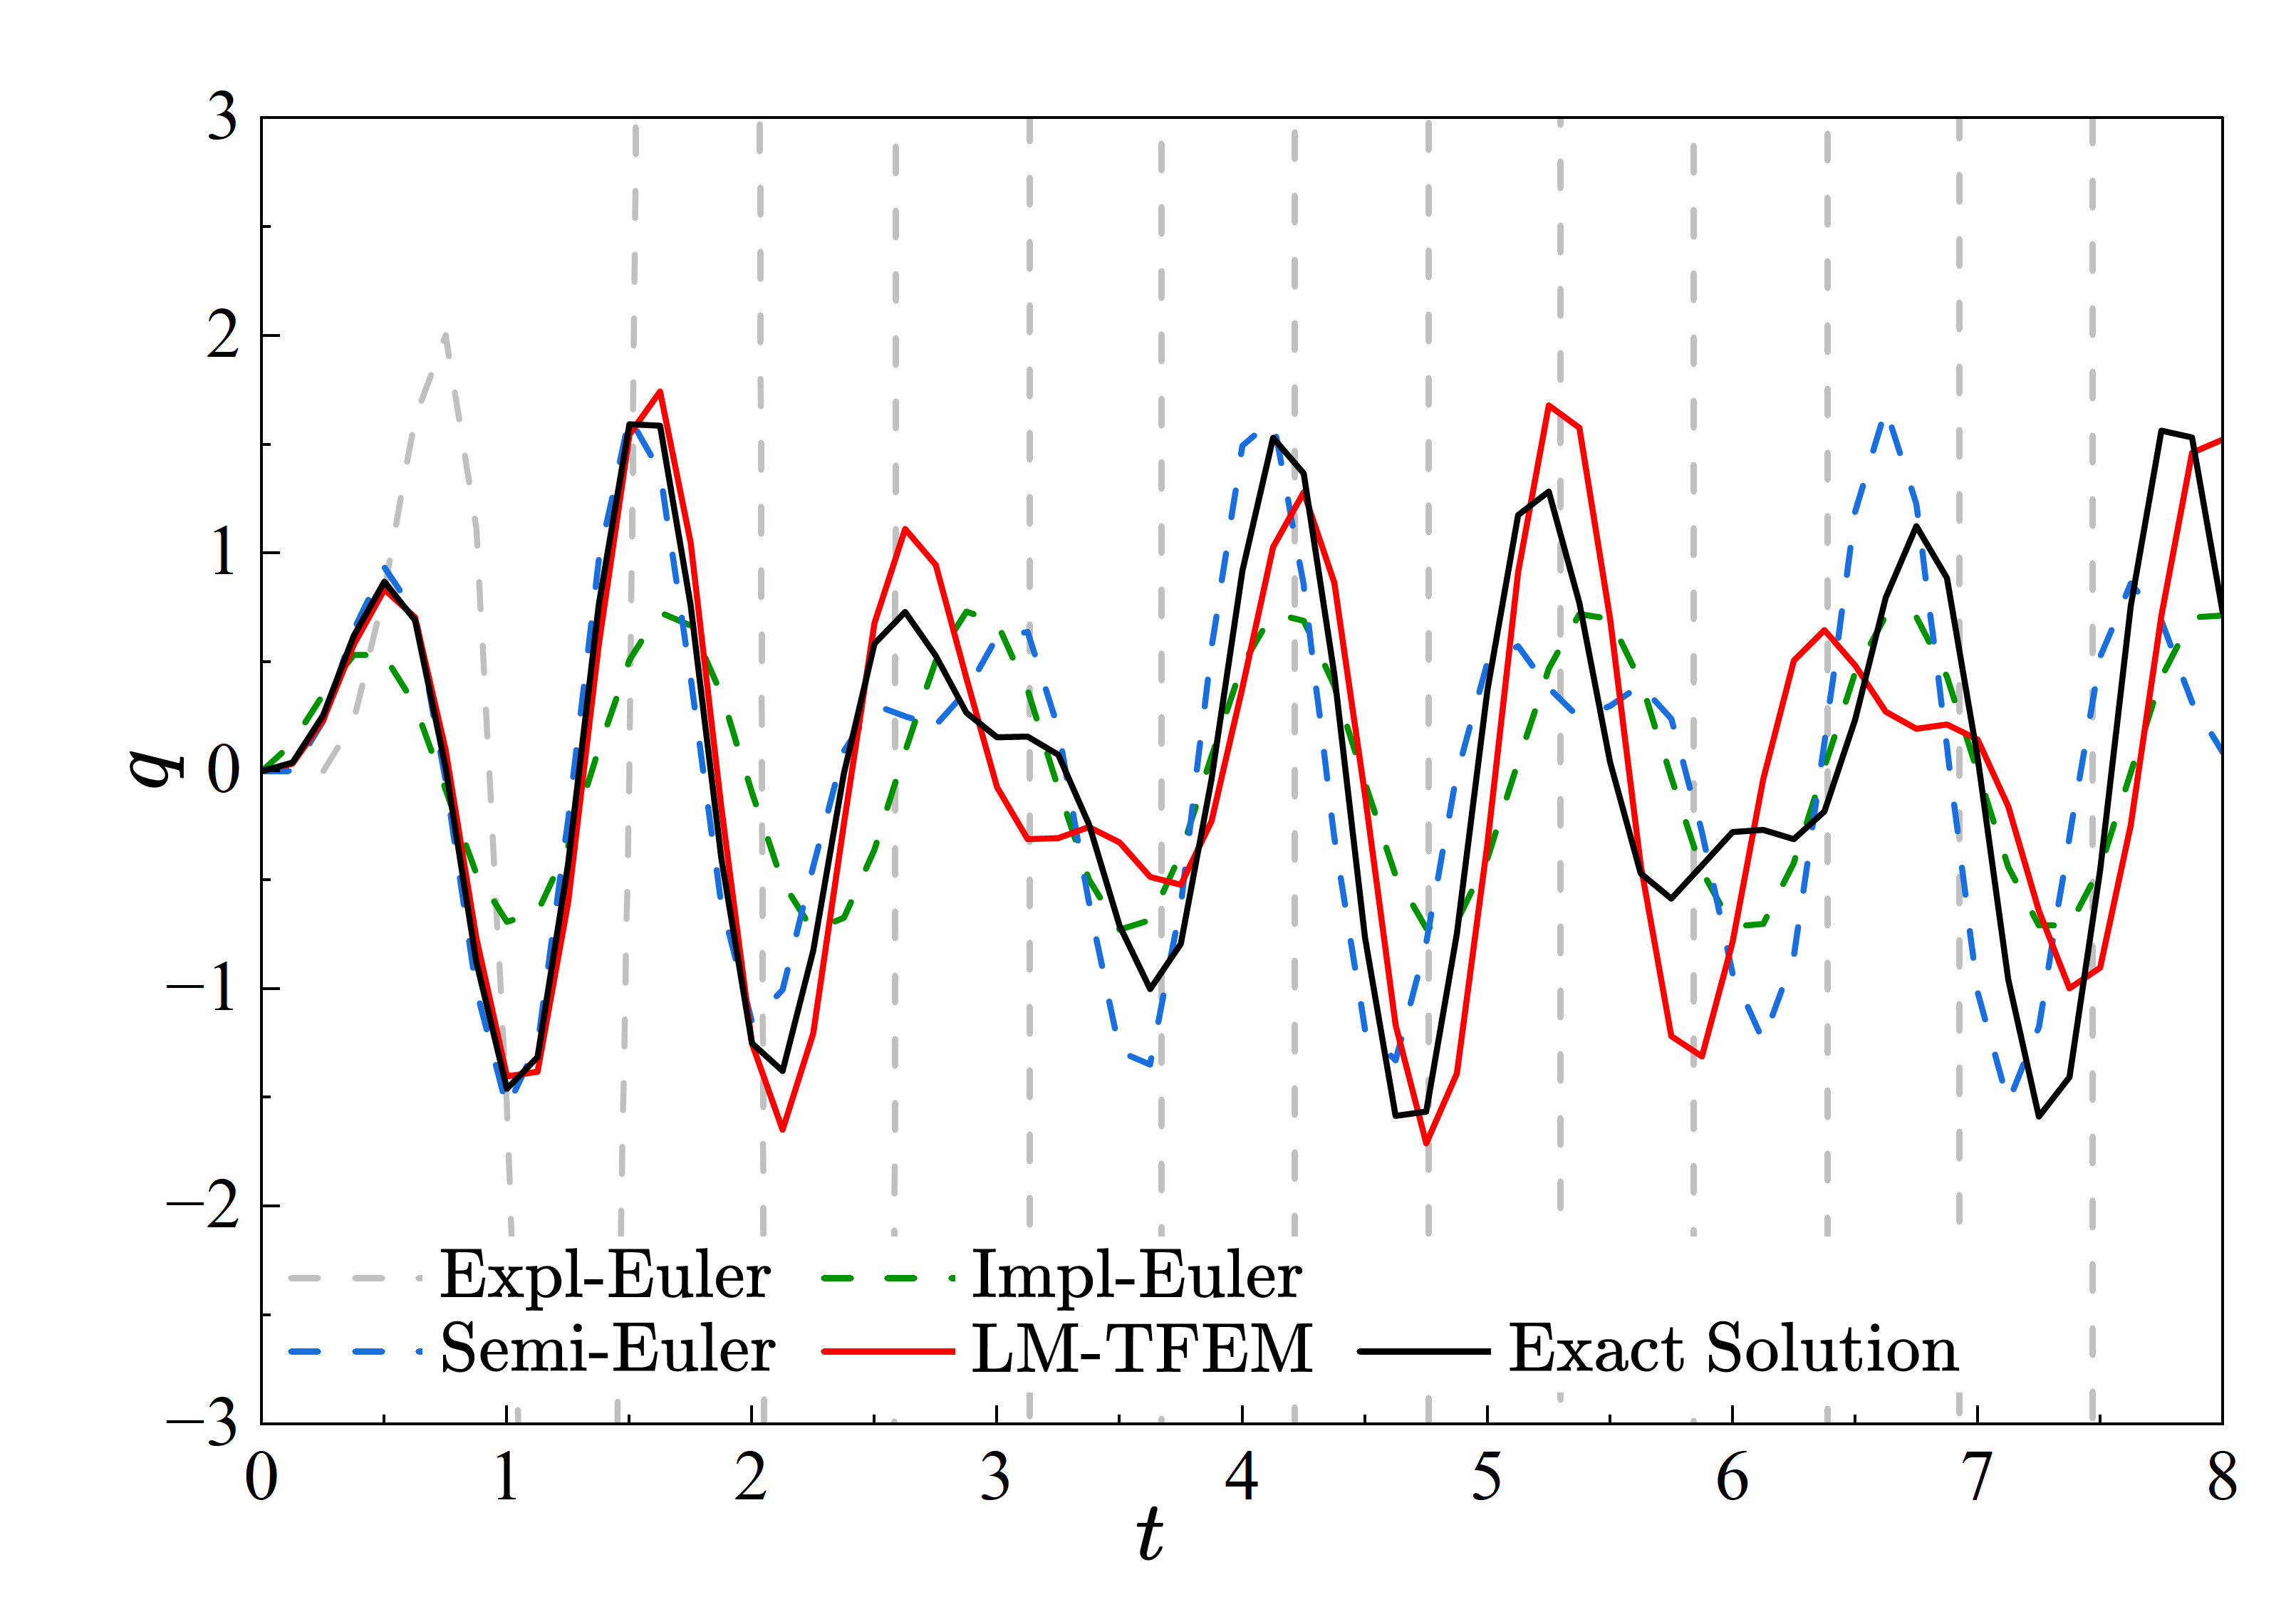
\includegraphics[width=0.45\textwidth]{fig/math/Δt=0.125简谐位移图.png} &
            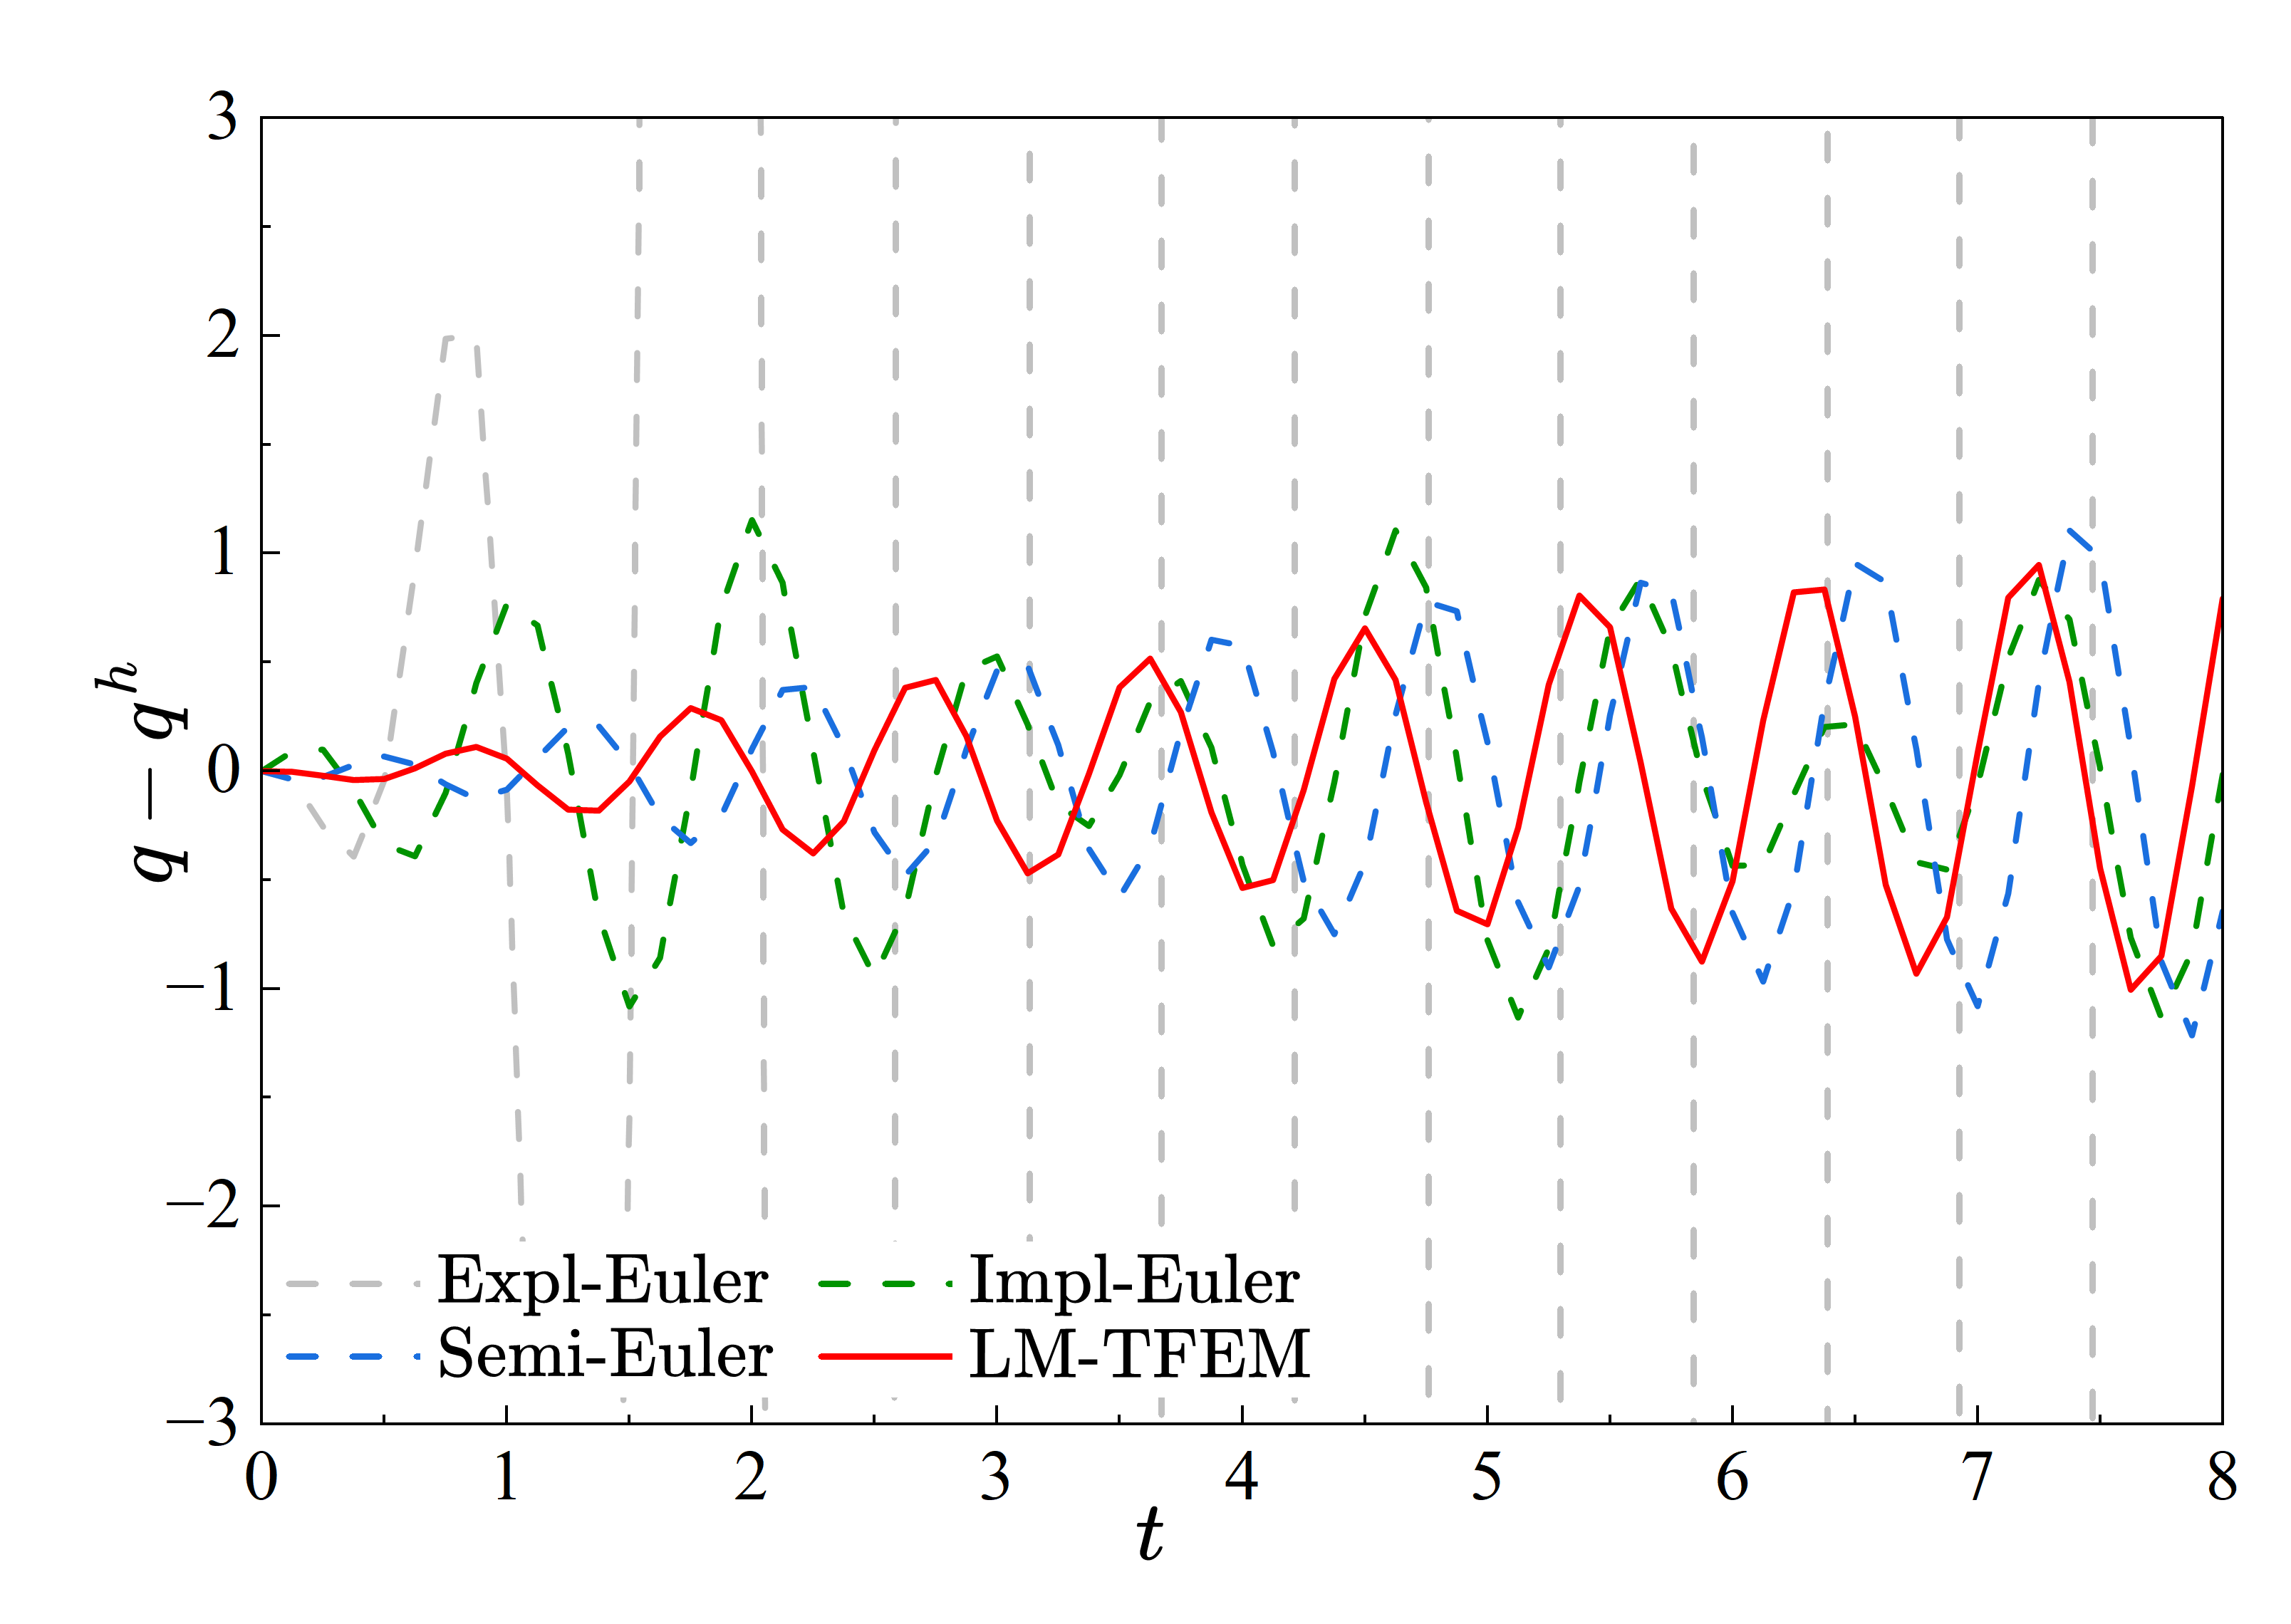
\includegraphics[width=0.45\textwidth]{fig/math/Δt=0.125简谐位移误差图.png} \\
        \end{tabular}
        \caption{$\Delta t=0.125$时四种方法计算简谐外力作用下弹簧小车问题的位移图与误差图}\label{fg:jx0.125}
\end{figure}
\begin{figure}[!h]
    \centering
        \begin{tabular}{c@{\hspace{15pt}}c}
            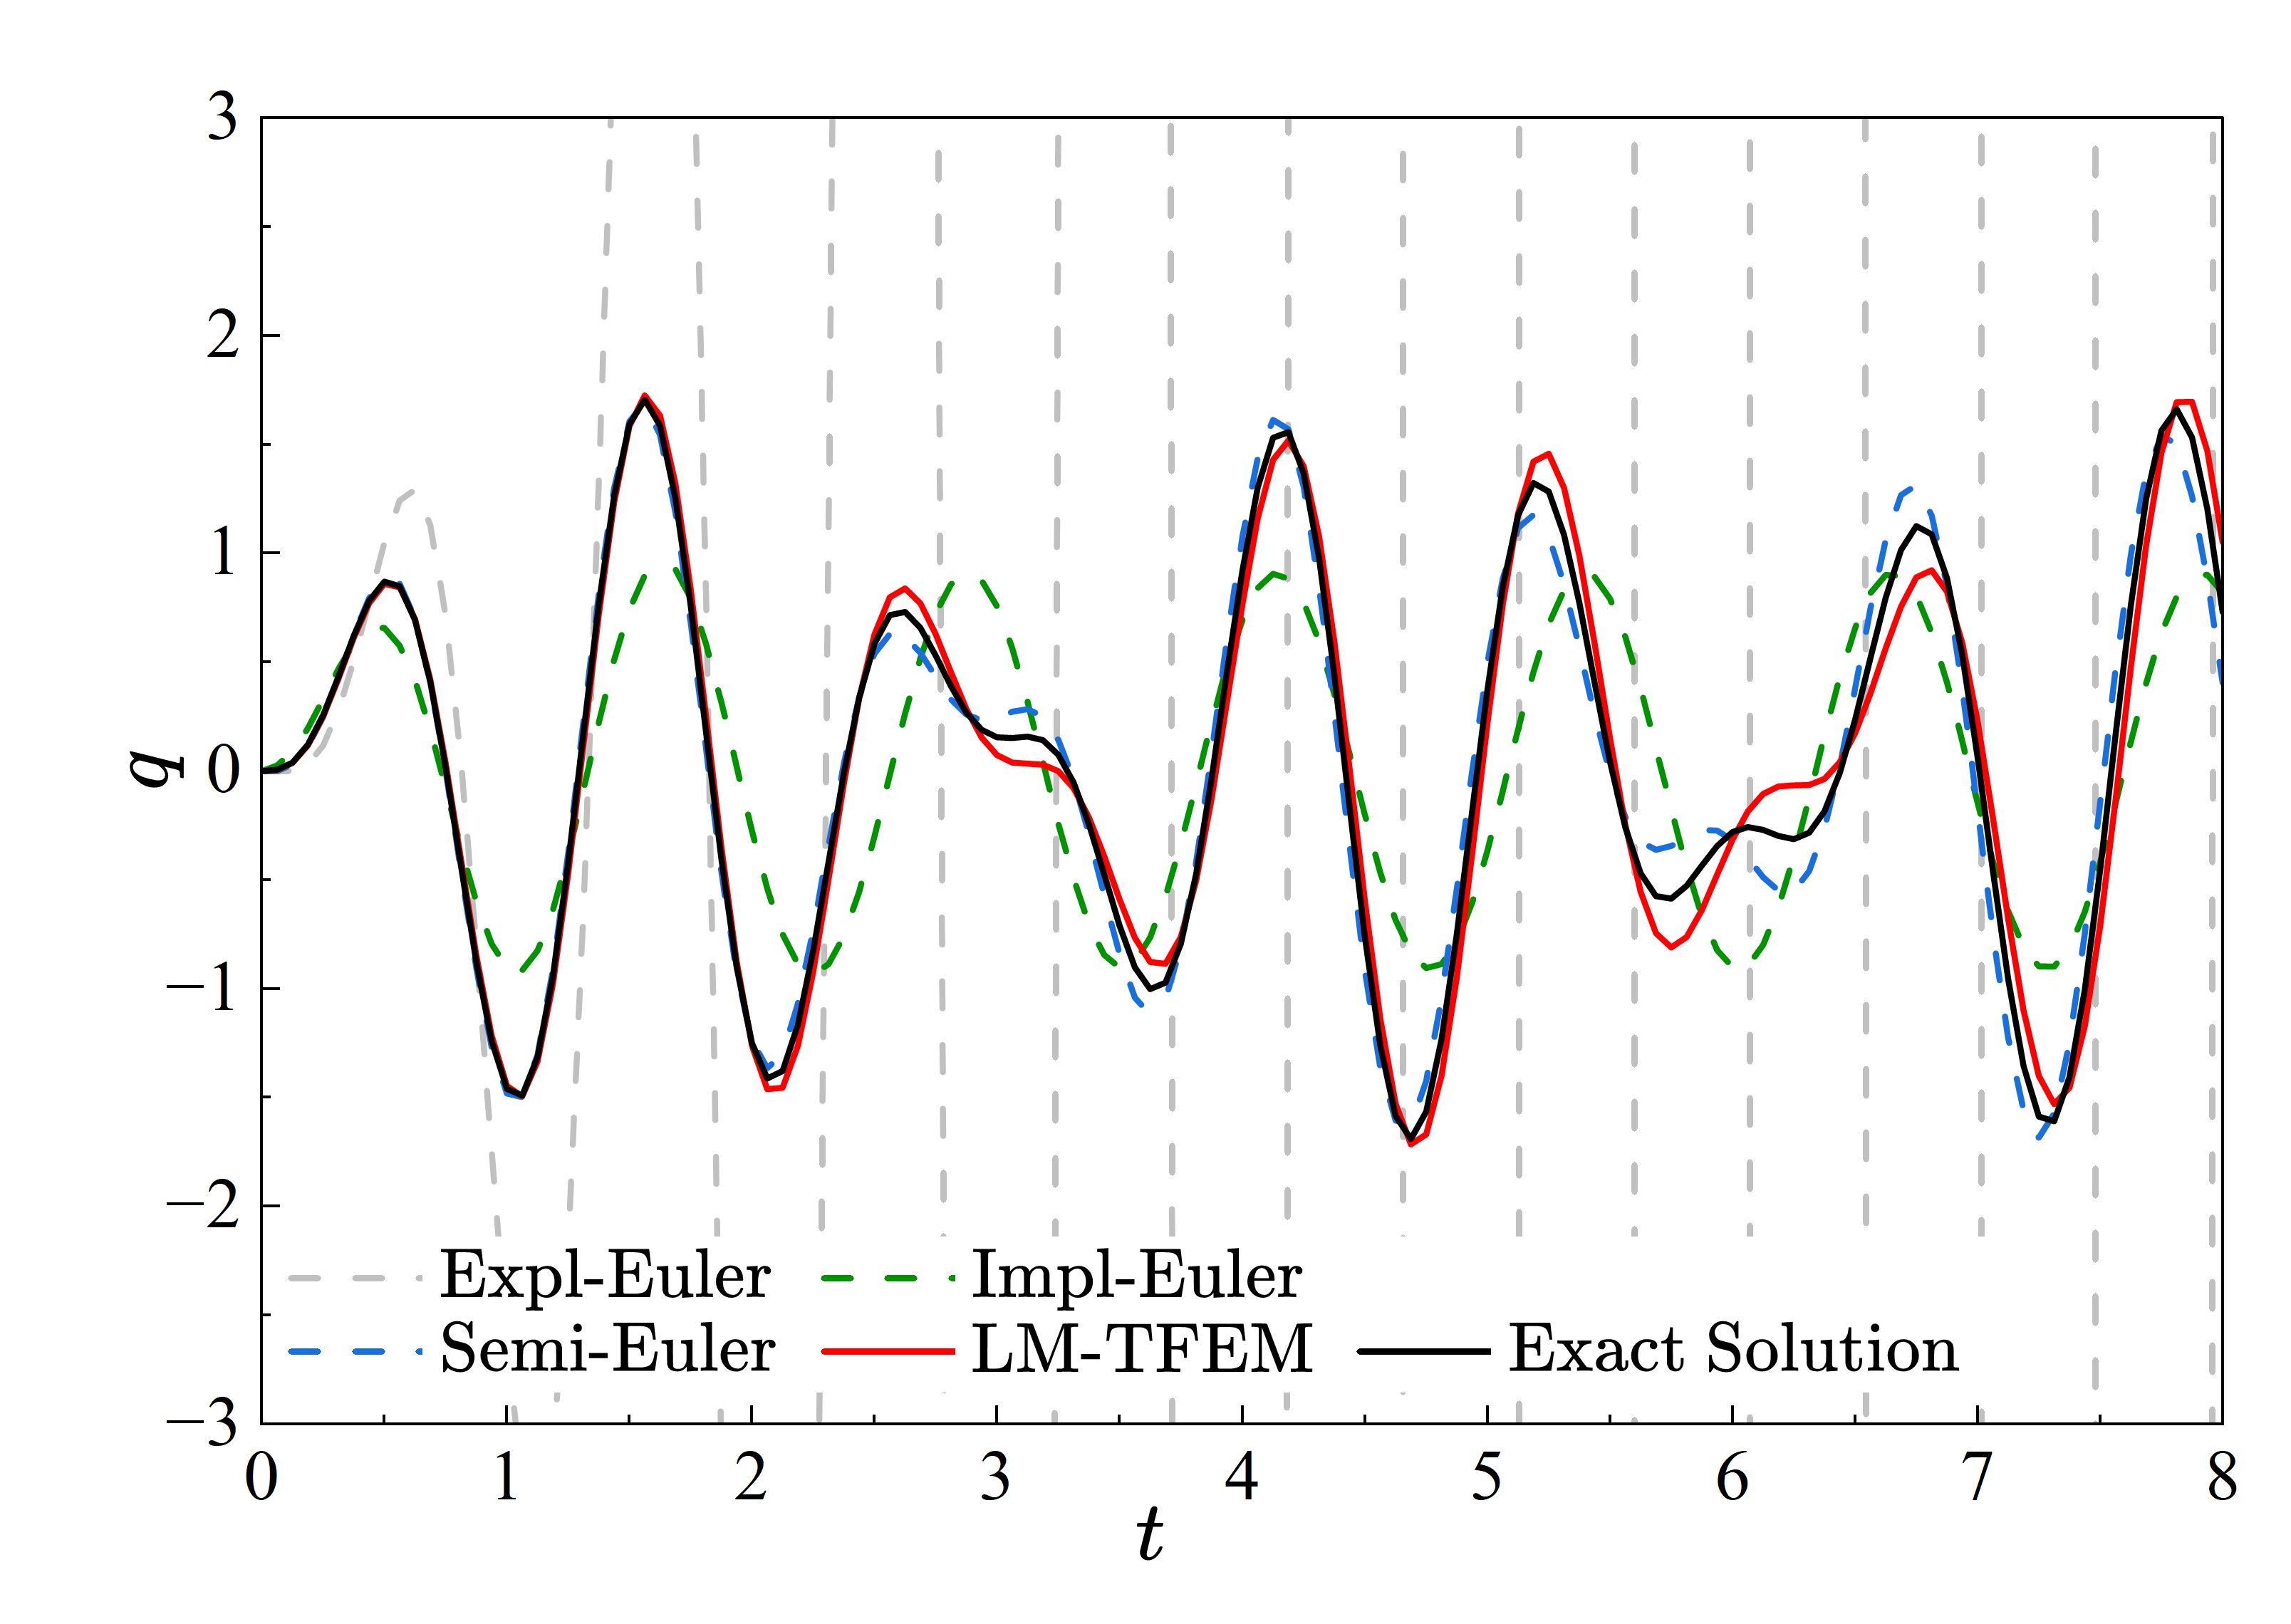
\includegraphics[width=0.45\textwidth]{fig/math/Δt=0.0625简谐位移图.png} &
            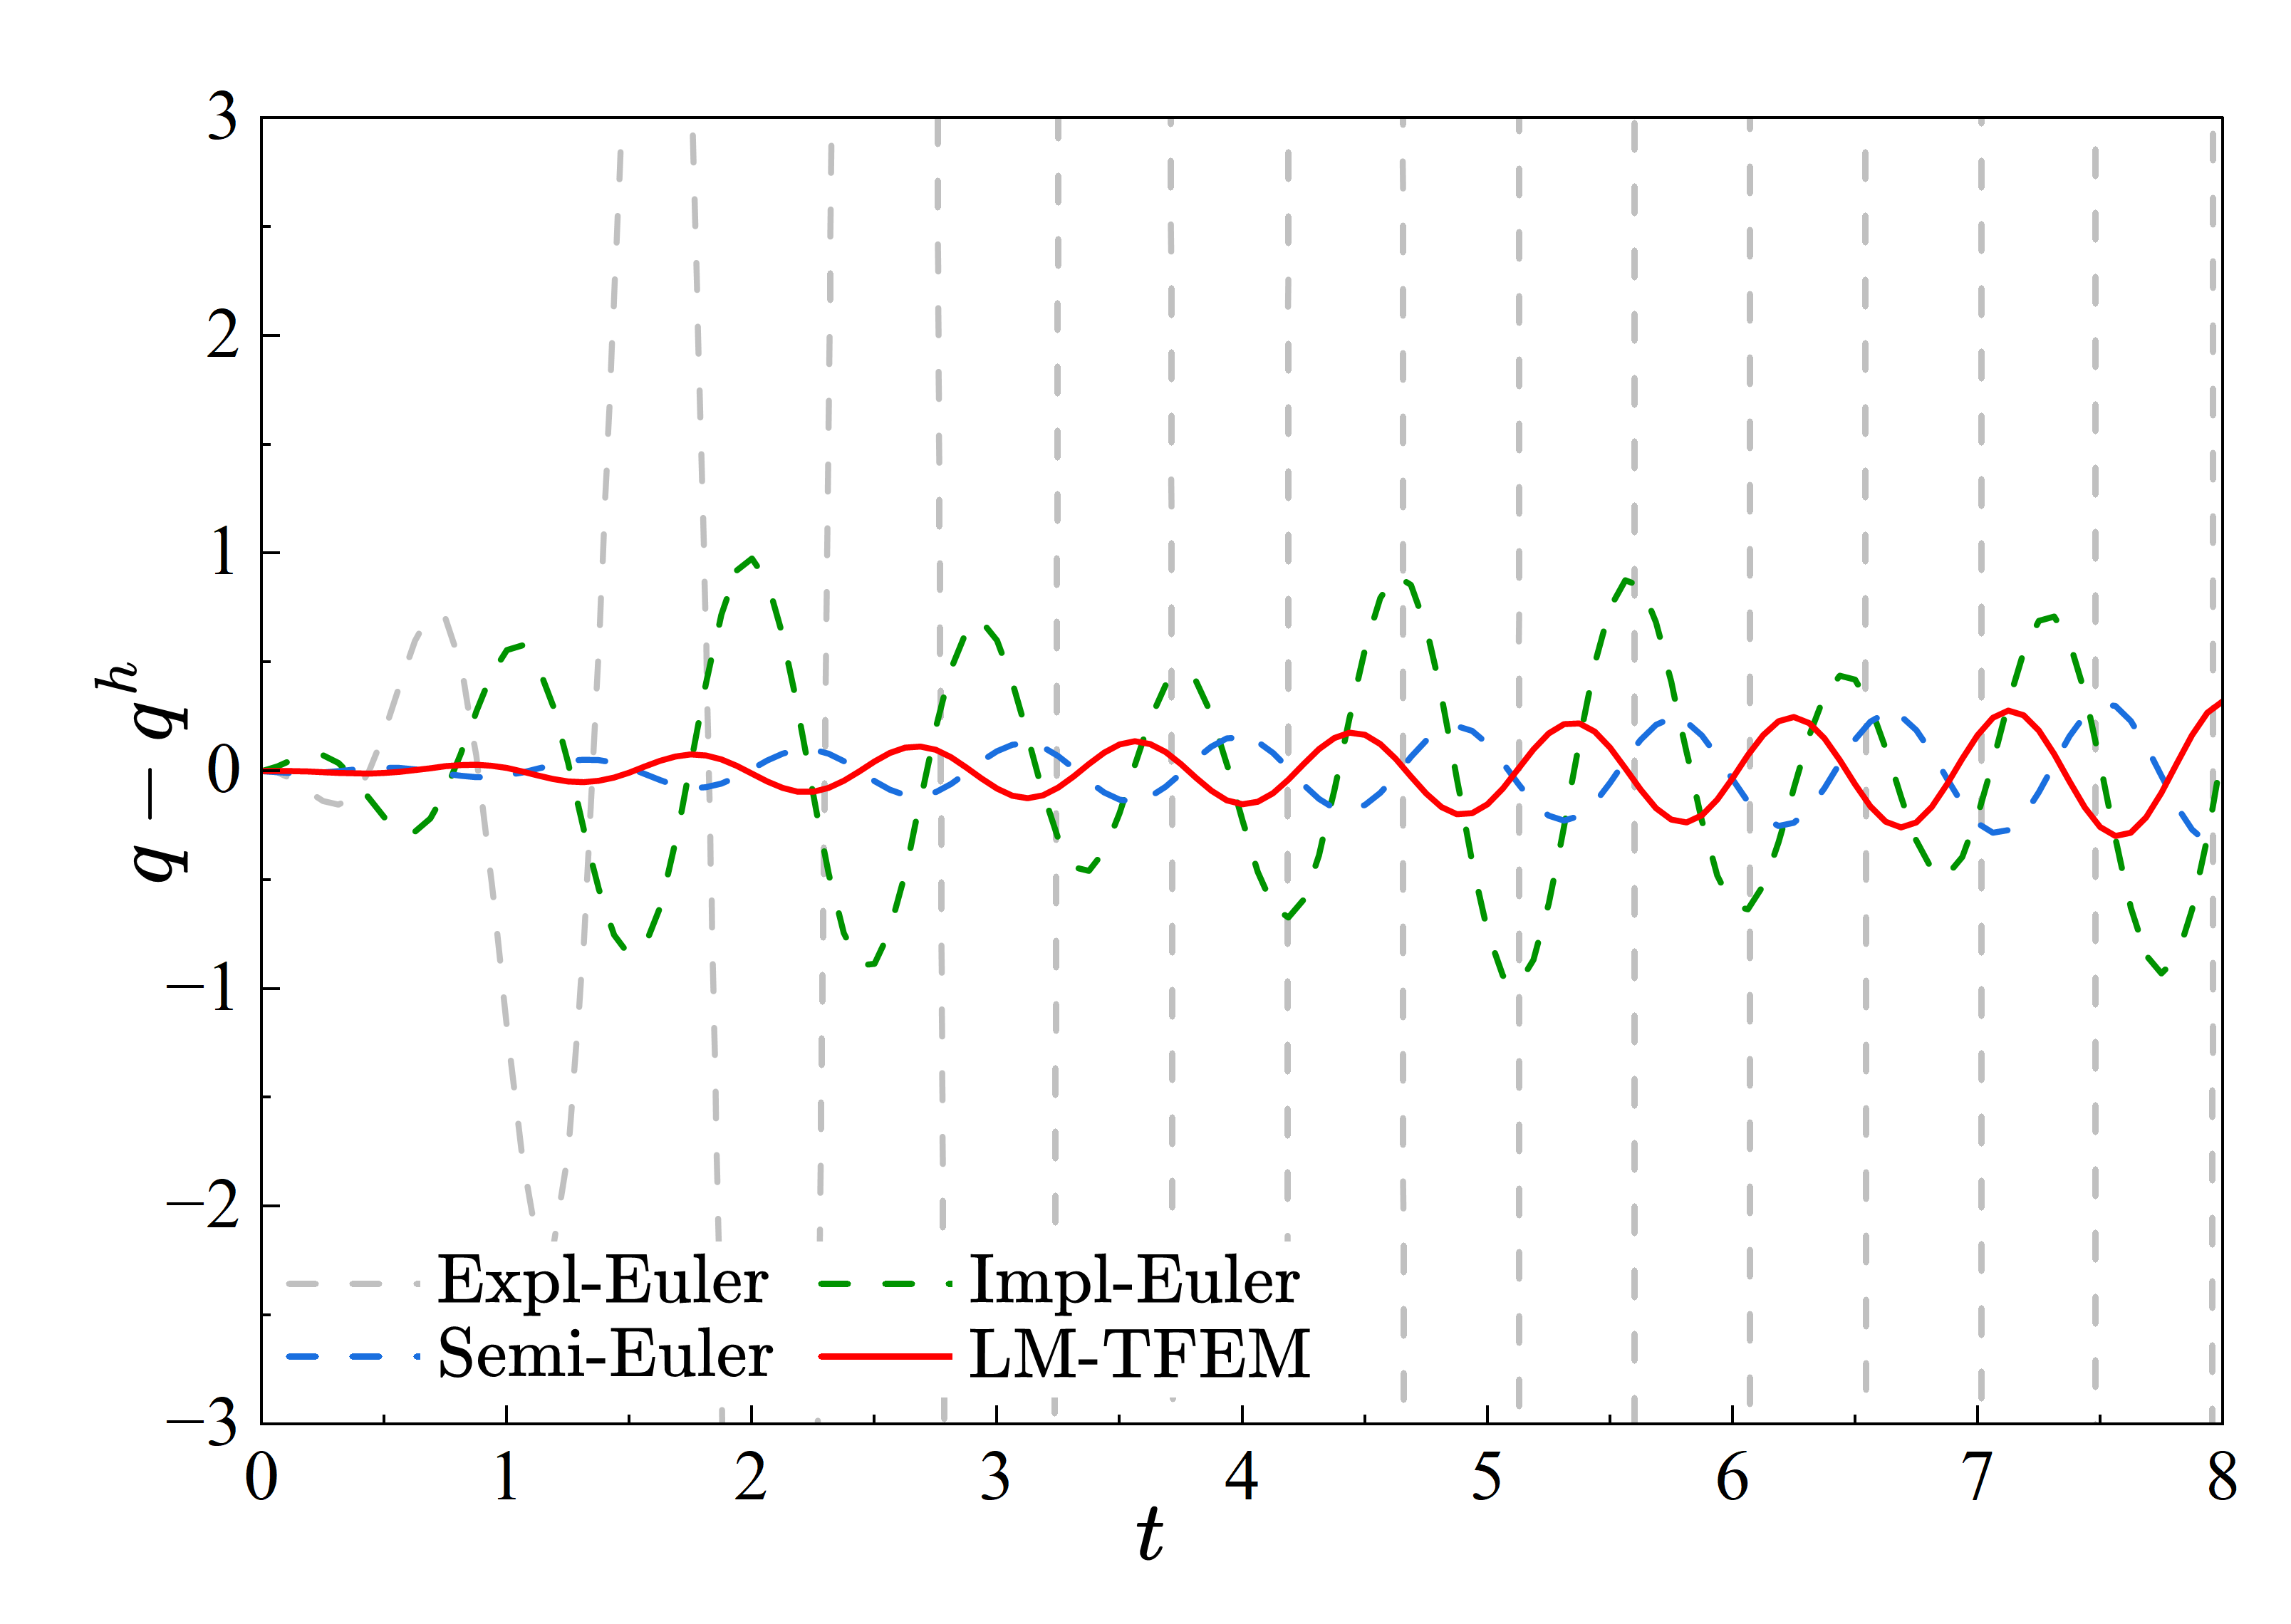
\includegraphics[width=0.45\textwidth]{fig/math/Δt=0.0625简谐位移误差图.png} \\
        \end{tabular}
        \caption{$\Delta t=0.0625$时四种方法计算简谐外力作用下弹簧小车问题的位移图与误差图}\label{fg:jx0.0625}
\end{figure}
\begin{figure}[!h]
    \centering
        \begin{tabular}{c@{\hspace{15pt}}c}
            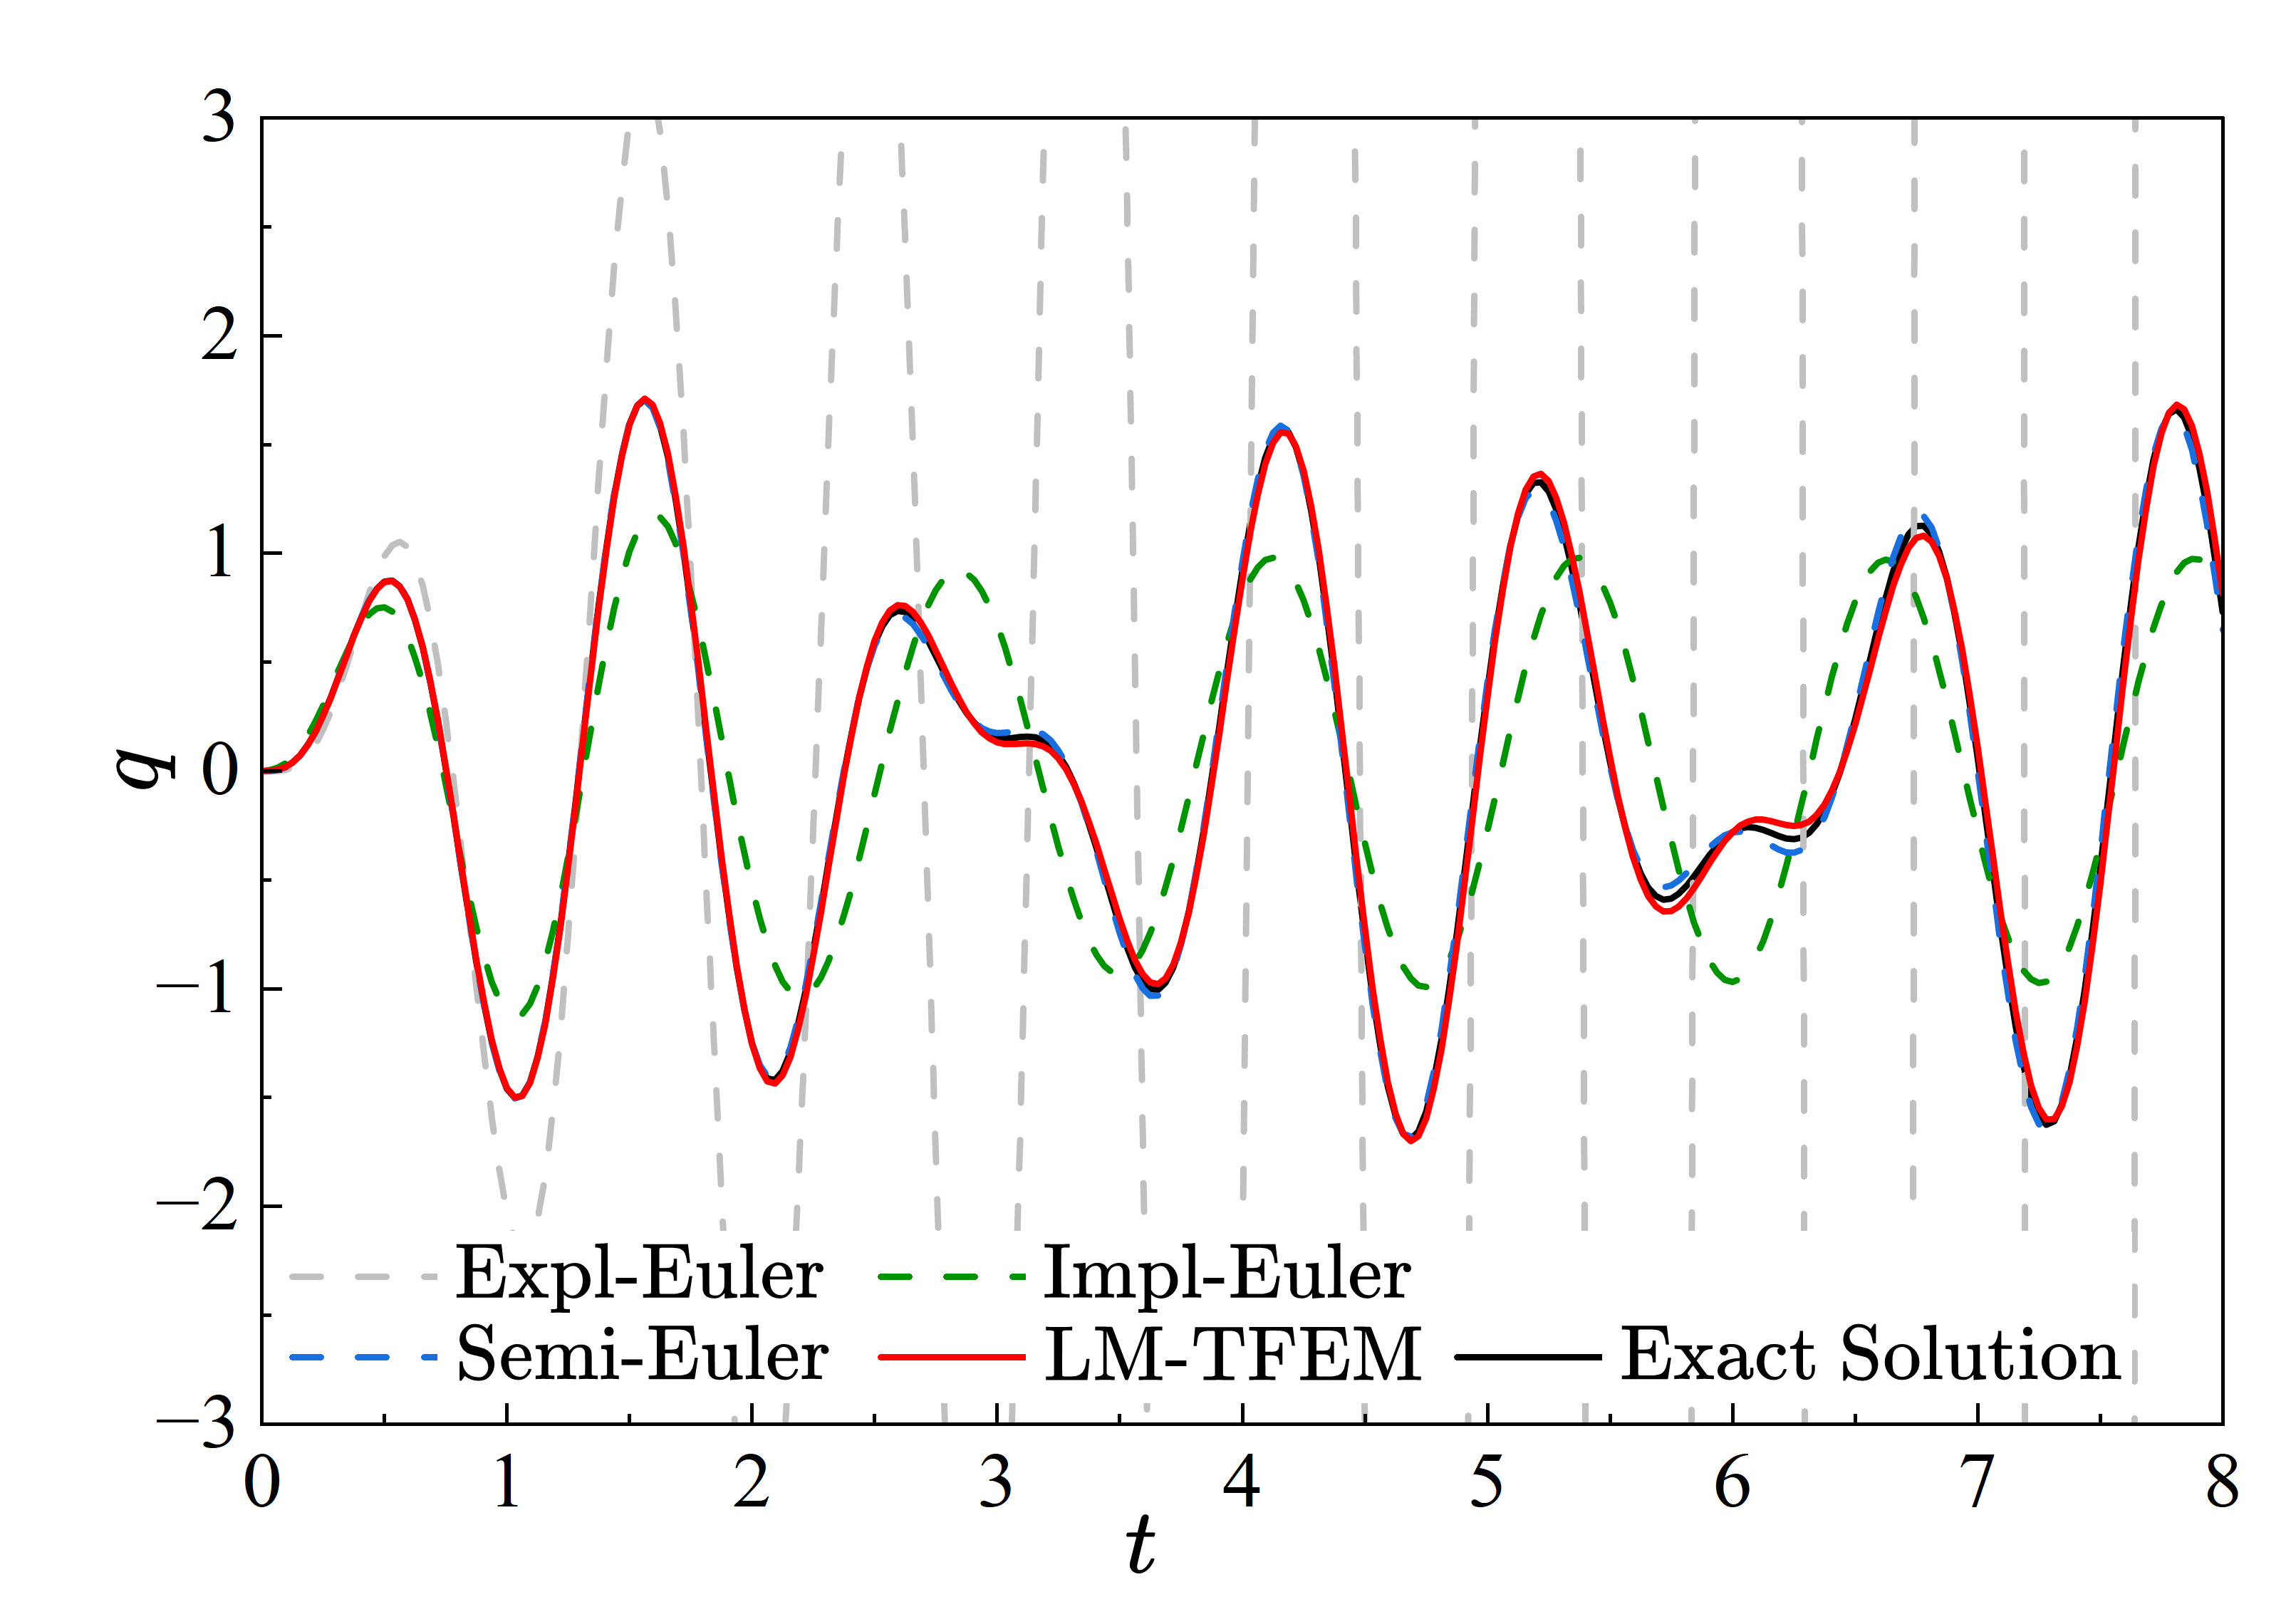
\includegraphics[width=0.45\textwidth]{fig/math/Δt=0.03125简谐位移图.png} &
            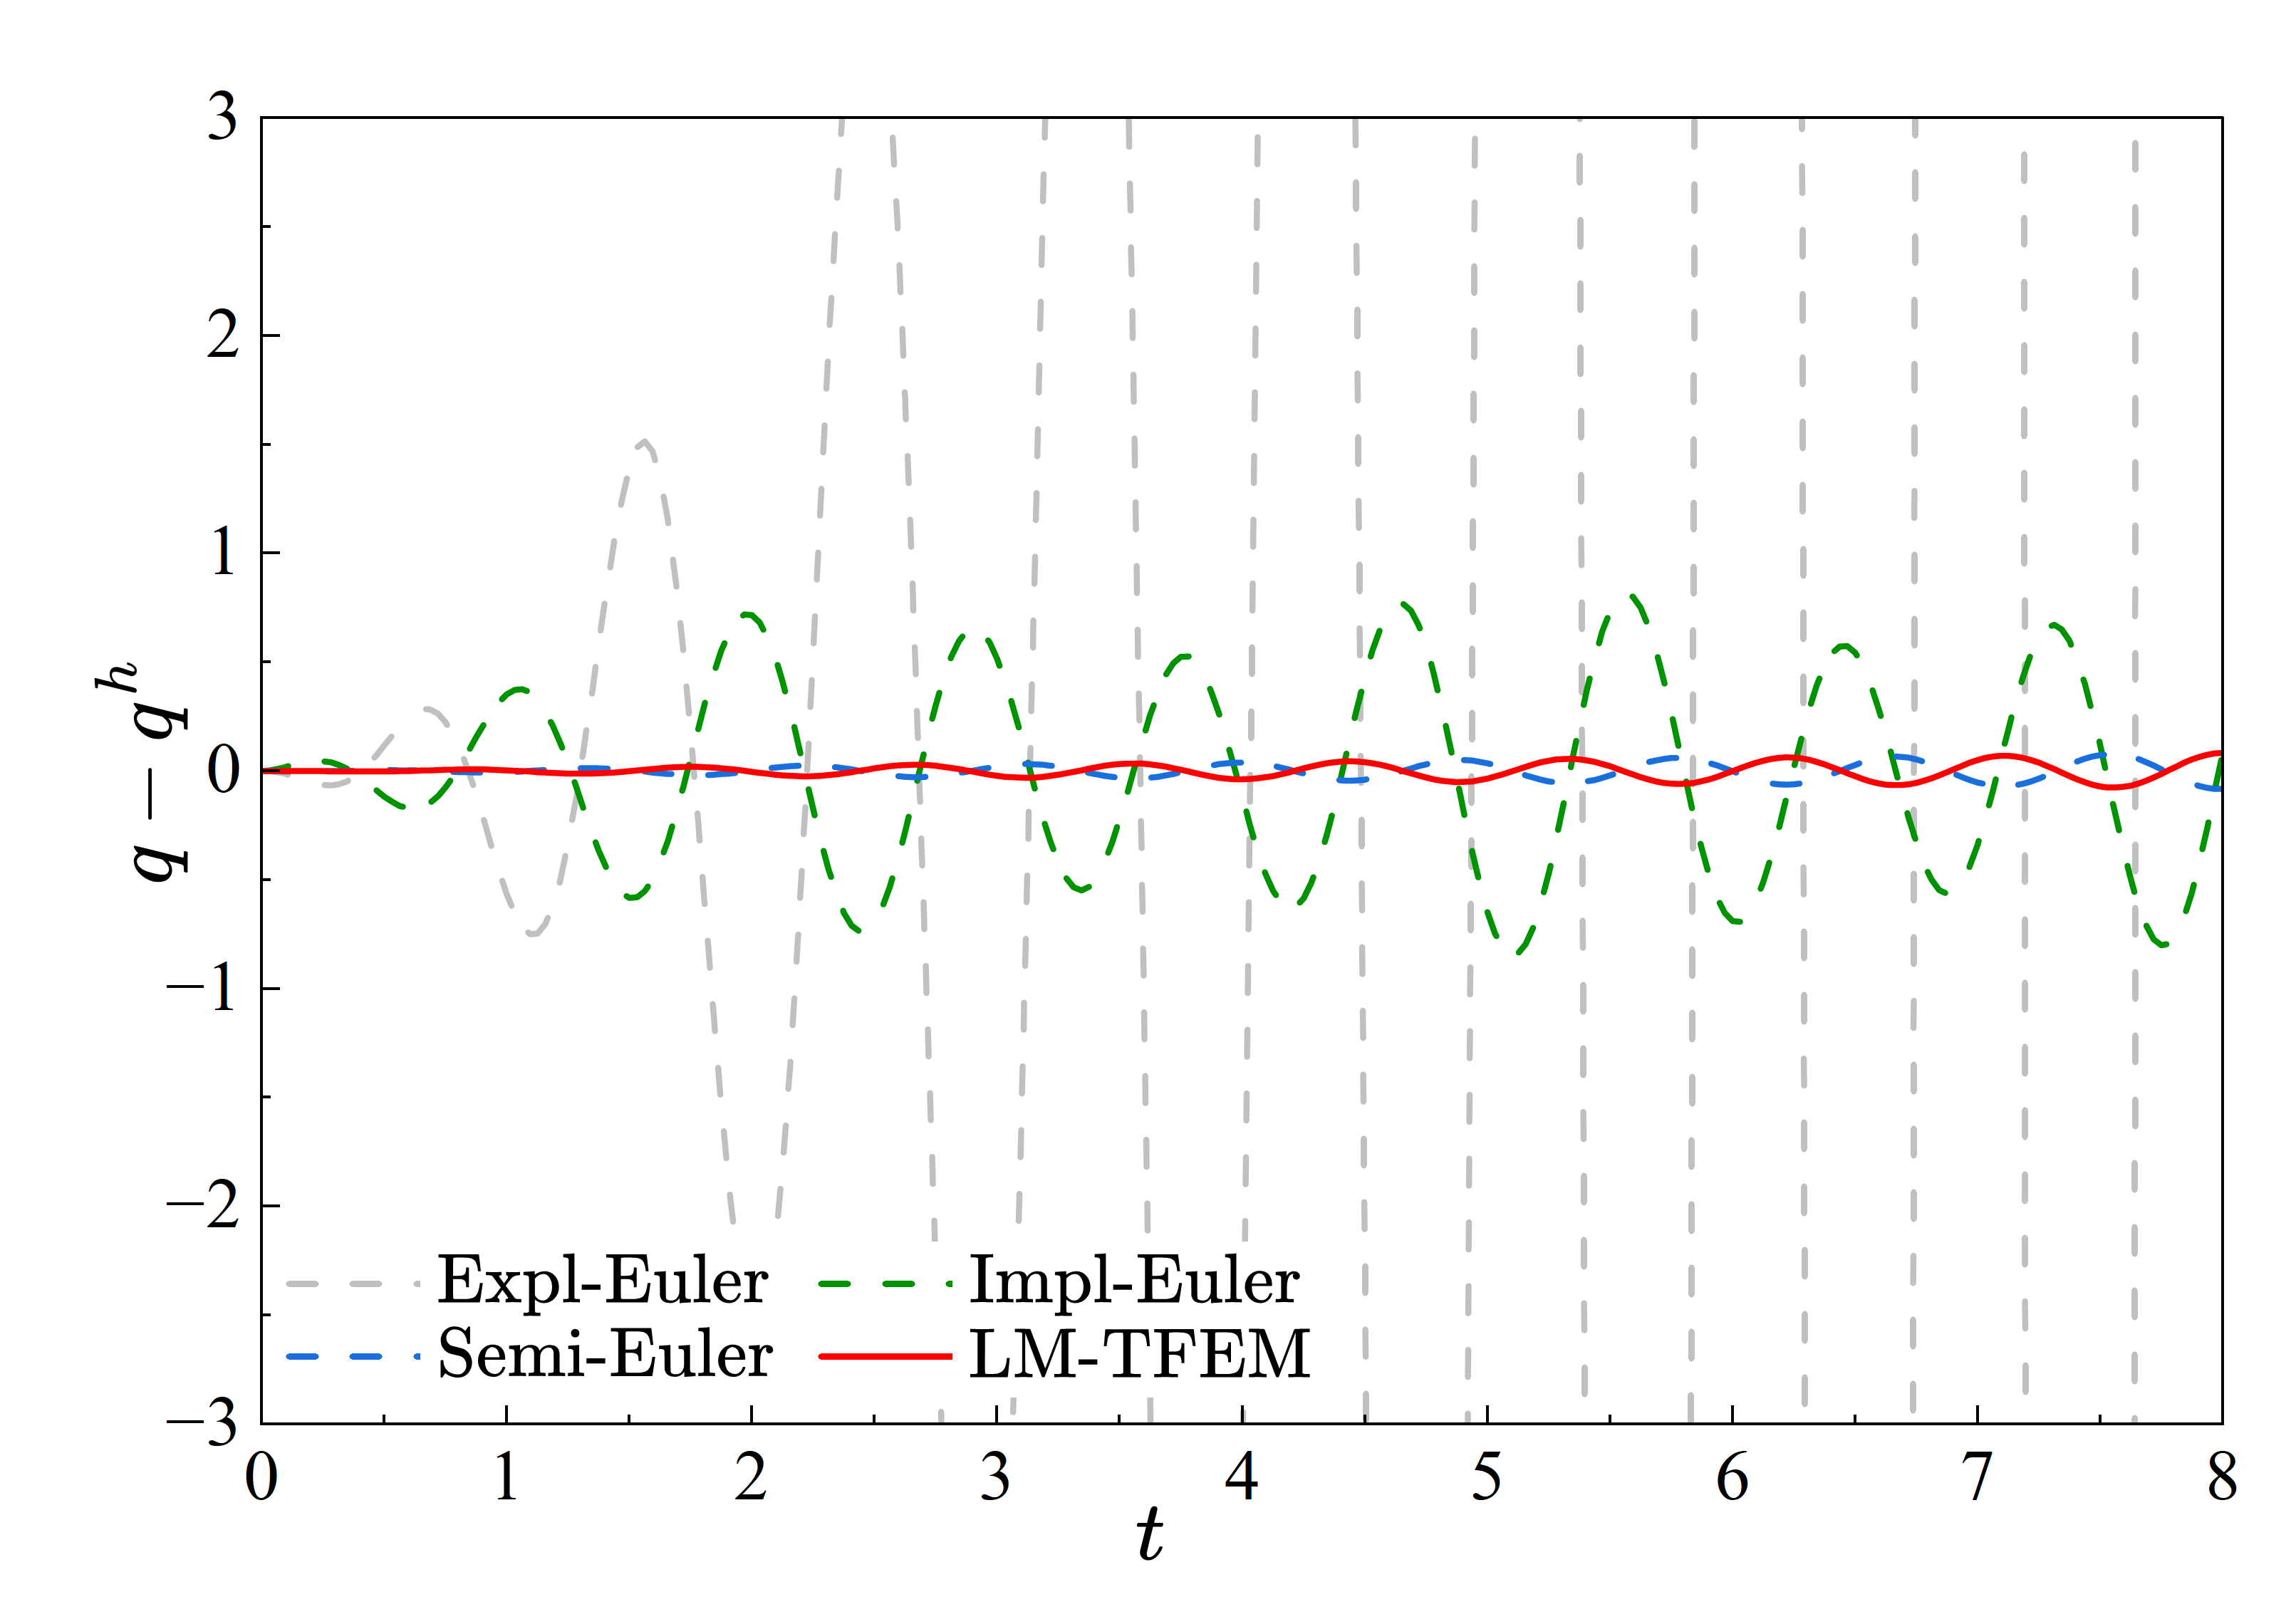
\includegraphics[width=0.45\textwidth]{fig/math/Δt=0.03125简谐位移误差图.png} \\
        \end{tabular}
        \caption{$\Delta t=0.03125$时四种方法计算简谐外力作用下弹簧小车问题位移图与误差图}\label{fg:jx0.03125}
\end{figure}

\begin{figure}[!h]
    \centering
    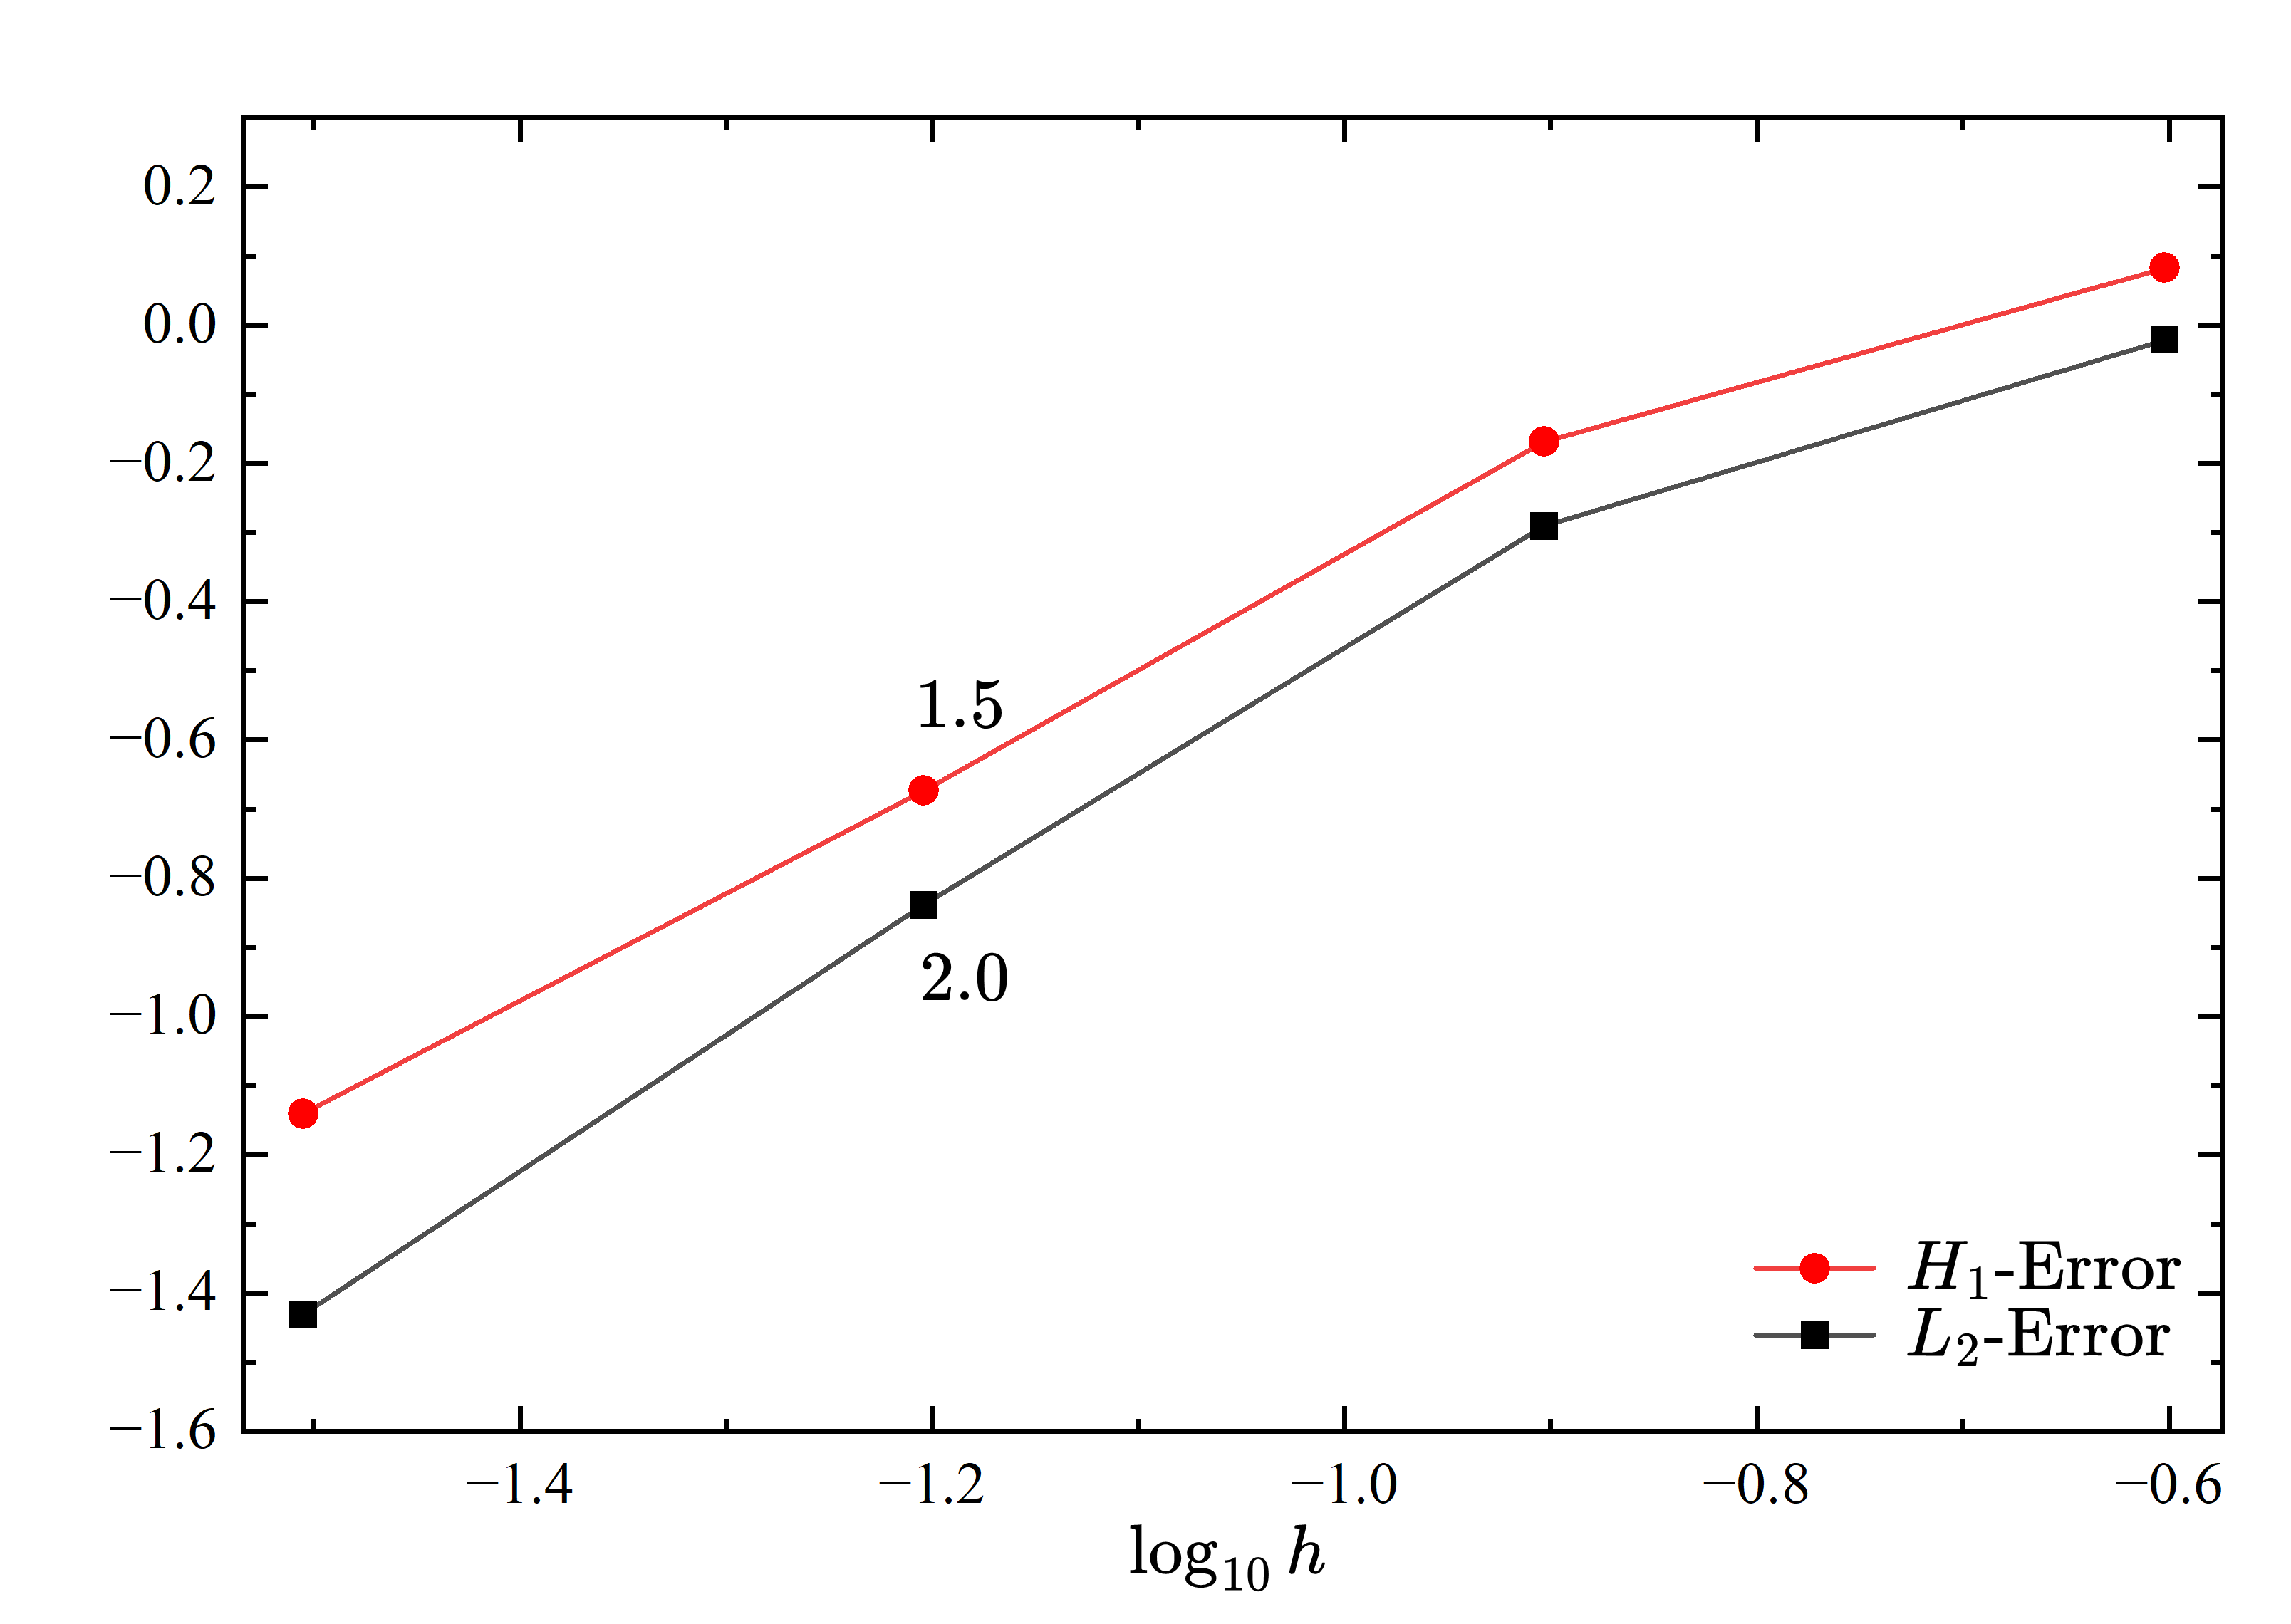
\includegraphics[scale=0.38]{fig/math/简谐波长根号50的L2收敛图.png}
\caption{\centering{在简谐外力作用下弹簧小车问题误差收敛结果}}
\label{fg:jxtanhuangxiaocheL2}
\end{figure}


\clearpage
\section{小结}

本章系统探究了动力问题的基于强形式的Newmark-$\beta$求解法和基于哈密顿原理的完全弱形式求解法，
对两种方法的数值计算结果进行了对比分析，
并探讨理论基于哈密顿原理求解法的时间末端边界问题及其解决方案。
首先，从强形式的控制方程出发，介绍了Newmark-$\beta$的三种方法，
三种方法均对时间域采用基于微分方程强形式离散分析。
随后，分析了基于哈密顿原理的完全弱形式伽辽金法在时间末端存在虚位移必须为零的边界问题，
并提出了一种基于拉格朗日乘子型的时域未端本质边界条件的施加方案来解决该问题，
通过引入一个拉格朗日乘数$p$代替原来无法数值实现的虚位移$\delta q$,
再将变分后的弱形式作为一个投影项加入到原来的能量泛函式里进行变分计算。
最后，通过对典型的弹簧小车算例的系统验证，证实了所提方案的优越性。
数值结果表明，该拉格朗日乘子变分求解方案不仅计算效率更高，
而且能够更好的确保数值计算结果的稳定性，同时具有最高的计算精度。
